\chapter{Old Chinese}\label{chapter-3.-chinese}

\paragraph{} Chinese enters history as the language written onto cattle or sheep
scapulae and turtle plastrons by the diviners of an archeological
culture centered at 小屯 Xiǎotún (c. 1200--1050 BCE). The decipherment
of these oracle bone inscriptions permits the identification of this
culture with the 商~Shāng dynasty of traditional Chinese historiography
(K. Chang 1980). Bone in­scrip­tions record questions concerning
weather, crops, warfare, and the regulation of the Shāng's complex
ritual life. Although they serve historians as invaluable sources
\citep{Keightley1978}, these short formulaic texts are difficult to
profitably use in historical linguistics. Linguistic research on the
language of the oracle bone inscriptions focusses primarily on syntax \citep{Takashima2000}.

The Shāng fell to their neighbors the 周 Zhōu (c. 1046 BCE). Although
scapulimancy is attested among the Zhōu, the younger dynasty is more
known for inscriptions in cast bronze ritual vessels \citep{Shaughnessy1991}.
Such bronze inscriptions, intended in part as family heirlooms,
typically record the appointment of the initial owner to public office.
Because the texts of some of these inscriptions rhyme and their
paleography is more obviously continuous with later forms of Chinese,
bronze inscriptions offer a more fruitful avenue for historical
linguistic research than do the earlier oracle bone inscriptions \citep{Behr2008}.

There is no doubt that the Shāng and Zhōu produced writings on more
perishable materials such as bamboo and silk; the character 冊 (pre-Qín 
\includegraphics[width=5mm]{Chapter5/ce4.png}
) for `book', attested already in bone inscriptions, portrays bamboo
strips bound together. Nonetheless, extant texts on silk and bamboo date
only from the Warring States period (5th century BCE) and later. These
excavated texts, which offer a much wider selection of genres than
either the bone or bronze inscriptions, are increasingly the subject of
research (e.g. \cite{Cook2012}), but historical Chinese phonology as
traditionally practiced makes use of much later sources. This
inattentiveness of phonologists to early sources is generally
reciprocated by the ignorance of historians and philologists concerning
recent progress in Chinese historical phonology \citep[]{Caboara2014}.

Five texts originating from before the 秦 Qín dynasty (221-206 BCE) have
enjoyed un­in­ter­rupted circulation to our own day. They are know as
the `five classics' \citep{Nylan2001}, on account of their status within the
Confucian tradition and their incorporation into the state curriculum
under the 漢 Hàn dynasty (206 BCE -- 220 CE). Within traditional Chinese
learning these texts enjoy a preeminence in the study of early China.
Nonetheless, like all documents with an ancient transmission they are
beset by problems of chronology, textual stability, and interpretation.
Because the 詩經  \emph{Shījīng} `Classic of Poetry' mostly consists of
rhymed poetry it is the one Classic to substantially inform the study of
historical phonology.

\section{Old Chinese}\label{old-chinese}

\paragraph{} The term `Old Chinese' has several senses that do not necessarily
converge; these senses include the language ancestral to all of the
Sinitic languages spoken today and the language spoken in the Shāng or
Zhōu polities. The most precise way of defining the language referred to
as `Old Chinese' is to point to the evidence used for reconstructing
this language. From this per­spec­tive, Old Chinese is three things: the
ancestor of Middle Chinese (\ref{par:middle-chinese}), the language reflected in the rhyming
practices of the \emph{Shījīng} (\ref{par:rhymes-of-the-Shijing}), and the language that informs the
structure of the Chinese script (\ref{par:structure-of-chinese-characters}). Many reconstruction systems rely
entirely on these three types of evidence (cf. 
\cite[11]{Schuessler2009minimal}).
However, the system of Baxter \& Sagart further includes the evidence of
some modern Chinese dialects (especially Mĭn), early loanwords from
Chinese into Hmong-Mien, Vietic, and Kra-Dai, and explicit discussions
of language in early Chinese texts 
\citep[2-4]{Baxter2014OldChinese}. The
work in your hands uses Old Chinese in the system of 
\citet[]{Baxter2014OldChinese}; the ensuing discussion presents a précis of this
system.\footnote{The system of Baxter \& Sagart has not met with
  universal endorsement. Positive reviews include \cite{Starostin2015},
  \cite{Goldstein2015}, and 
  \cite{Hill2017OCreview}.
  Negative reviews include
  Schuessler 2015, 
  \cite{Ho2016}, and 
   \cite[]{Harbsmeier2016}. On the one hand many
  criticisms apply \emph{mutatis mutandis} to all six vowel systems \citep[esp. pp. 183-184]{Ho2016} or even to all efforts in historical
  linguistics \citep[esp. pp. 484-487]{Harbsmeier2016}. On the other hand
  some criticisms concern details only
  \citep[]{Schuessler2015BSrv}. Replies to the
  negative reviews are in press. I discuss some reasons for my choice of
  Baxter \& Sagart's system below (cf. §). An additional benefit of
  their system is that it is easily converted into simpler systems, such
  as Schuessler's 
  \citeyearpar[]{Schuessler2009minimal}, whereas it is not straightforward to convert a
  simpler system into Baxter \& Sagart's.}

Baxter \& Sagart's own presentation of their system is necessarily more
authoritative than the summary here, but my restatement may nonetheless
prove helpful because of its distinct expository approach. I aim to show
how the reader may herself reconstruct Old Chinese. Consequently, the
organization is built around the types of evidence that contribute to
Old Chinese reconstruction. In contrast, Baxter \& Sagart present a
reconstructed system as a system, combining all possible sources of
evidence in favor of the system's architecture at all points in the
argument.

In the ensuing presentation, I first discuss each type of evidence
(\ref{par:middle-chinese}-\ref{par:morphological-speculation}). Next comes a survey of the simplex initials, built on the basis
of the three traditional sources (\ref{par:lex-initials-of-old-chinese}-\ref{par:t-p-initials-before-ufvulars-as-a-source-of-MC-velars}). Thereafter follows treatment of
those elements of Baxter \& Sagart's system, generally the
'pre-initials', buttressed by the less traditional sources (\ref{par:recon-t-p-initials-on-morphological-speculation}-\ref{par:reconstructing-loose-pre-initials}). Again
relying on the three traditional sources, come discussion of the medial
(\ref{par:old-chinese-medial-r-}), vowels (\ref{par:old-chinese-vowels}-\ref{par:Asymmetries-in-type-B-rimes-with-dental-codas}), tones (\ref{origins-of-the-tones-and-final-clusters}-\ref{par:origin-of-the-rising-tone}), and final consonants (\ref{par:finals-of-old-chinese}-\ref{par:final-r}).


\subsection{\texorpdfstring{Rhymes of the 詩經
 \emph{Shījīng}}{Rhymes of the 詩經 Shījīng}}
 

\paragraph{}
\label{par:rhymes-of-the-Shijing}
The earliest received Chinese text containing rhymed poetry is the
詩經  \emph{Shījīng}. The collection consists of 305 poems presumed to
date from the 11th to 7th centuries BCE. Reading the poems of the
 \emph{Shījīng} aloud in the pronunciation of Peking today, it is
clear that many of the poems are intended to rhyme; many of the rhymes
are still good. Nonetheless, in many cases the pattern of rhyming also
makes clear that some words are meant to rhyme that fail to do so in
today's pronunciation. To illustrate this point Baxter draws attention
to Ode 8 
\citeyearpar[151]{Baxter1992}. Words in small capitals are the rhyme words.

\begin{quotation}
\noindent
采采芣苢、cǎi cǎi fóu yǐ\\
薄言采之。bó yán cǎi zhī\\
采采芣苢、cǎi cǎi fóu yǐ\\
薄言有之。bó yán yǒu zhī\\
\vspace{2mm}
\noindent
采采芣苢、cǎi cǎi fóu yǐ\\
薄言掇之。bó yán duō zhī\\
采采芣苢、cǎi cǎi fóu yǐ\\
薄言捋之。bó yán luō zhī\\
\vspace{2mm}
\noindent
采采芣苢、cǎi cǎi fóu yǐ\\
薄言袺之。bó yán jié zhī\\
采采芣苢、cǎi cǎi fóu yǐ\\
薄言襭之。bó yán xié zhī\\
\vspace{2mm}

\noindent Colorful is the plantain, we gather it;\\
colorful is the plantain, we hold it.

\vspace{2mm}
\noindent Colorful is the plantain, we pick it;\\
colorful is the plantain, we pluck it.

\vspace{2mm}
\noindent Colorful is the plantain, we take it in our held-up flaps;\\
colorful is the plantain, we take it in our tucked-up flaps.\\
\end{quotation}

The pattern of rhymes makes clear that 采 \emph{cǎi} and 有  \emph{yǒu}
are intended to rhyme, but as their romanization reveals these syllables
do not rhyme in the standard pro­nun­ci­a­tion of Peking today. The
Middle Chinese pronunciations of these characters, 采  \emph{tshojX} and
有  \emph{hjuwX}, also fail to rhyme.

Such failures of the poems to rhyme where expected have been noticed
since at least the sixth century of our era, when 沈重 Shěn Zhòng
suggested adjusting one's pro­nun­ci­a­tion to make the rimes of the
 \emph{Shījīng} work. Lù Démíng 陸德明 (550?-630) criticized this view,
instead explaining that 古人韻緩，不煩改字``the ancients rhymed loosely,
one need not trouble to change the words'' (Baxter 1992: 163 and note
105 on p. 829). The 明 Míng dynasty scholar 陳弟Chén Dì (1541-1617)
explained that sound change had altered the original pro­nun­ci­a­tion
of at least some words, and that these words normally had a single
pro­nun­ci­a­tion in the mouths of the ancients, even if a
pro­nun­ci­a­tion different from that of his own day 
\citep[154]{Baxter1992}.
Chén Dì appears to have believed that  \emph{chaque mot a son histoire}
and did not systematically explore the difference between ancient
phonological categories and those of his own day. The scholar 顧炎武 Gù
Yánwǔ (1613-1682) was first to undertake a reconstruction of the rime
categories of Old Chinese; he elaborated ten rime categories (韻部
 \emph{yùnbù}) in the \emph{Shījīng}, which split into the more elaborate
categories of Middle Chinese rimes 
\citep[155-157]{Baxter1992}. Subsequent
scholars distinguished categories that the \emph{Shījīng} keeps apart in
its rhyming practices, which 顧炎武 Gù Yánwǔ had failed to notice. The
categories re­cog­nized by scholars working within the Chinese
philo­logical tradition steady rose over time to 22.\footnote{Jiāng Yǒng
  江永 (1680-1762) recognized 13 categories, 段玉裁 Duàn Yùcái
  (1735-1815) recognized 17 categories, 江有誥 Jiāng Yǒugào (d. 1851)
  recognized 21 categories, and finally 王力 Wáng Lì (1900-1986)
  recognized 22 categories, cf. 
  \citet[157-171]{Baxter1992}.} As Baxter
remarks ``it is easy to spot Old Chinese rhymes that would not have been
allowed in Middle Chinese; but Old Chinese rhyme distinctions among
words which did rhyme in Middle Chinese are easily overlooked'' 
\citep[159]{Baxter1992}. In the late 20th century, armed with the six vowel hypothesis of
Old Chinese, motivated by the internal reconstruction of Middle Chinese
(§§-), the three scholars 鄭張尚芳 Zhèngzhāng Shàngfāng (1987), Sergei
Starostin 
\citeyearpar[]{Starostin89}, and William Baxter 
\citeyearpar{Baxter1992} independently recognized
many more rime categories. For example,
\citet[]{Schuessler2009minimal}, who also
operates in the six-vowel tradition, puts the total number of Old
Chinese rime categories at 38 and I count 45 in Baxter \& Sagart's 2014
book. 
\citet[]{Baxter1992} gives detailed statistical evidence that the
 \emph{Shījīng} indeed distinguishes the more recently proposed
categories that result form the six vowel hypothesis.

The rime category of an Old Chinese word is only directly knowable if
that word happens to occur as a rhyme word in the
 \emph{Shījīng}.\footnote{Explicit analyses of  \emph{Shījīng} rhymes
  include 
  \citet{Karlgren1950},
  \citet{Wang1980a}, 
  \citet[583-743]{Baxter1992}, and \citet[]{Wang2011Shijing}.} Except for in those few cases where the Middle
Chinese pronunciation of a word may, according to one's overall theory,
develop only from a single Old Chinese rime category, in order to speak
of the rime category of words that do not appear as rhyme words in the
 \emph{Shījīng} one must turn to the phonetic information inherent in the
Chinese script.

\subsection{Structure of Chinese
characters}

\paragraph{} 
\label{par:structure-of-chinese-characters}
A Chinese character is normally analyzable into a phonetic component
and a semantic component. For example, the character 被 (18-16e), which
writes the word \emph{bjeX} `cover oneself with' is com­posed of the
phonetic component 皮 (18-16a), which as a character itself represents
the word  \emph{bje} `skin', and the semantic component 衤, a con­tracted
version of 衣 (27-05a) `clothes'. The pronunciations \emph{bjeX} and
 \emph{bje} differ only in tone. The meaning `clothes' is sufficient to
dis­tinguish \emph{bjeX} `cover oneself with' from 疲 \emph{bje} `weary'
or 陂~ \emph{pje} `dam'. To take another example, the character 銳
 \emph{ywejH} (22-13f) `sharp' is composed of the phonetic 兌
 \emph{dwajH} (22-13a) and the semantic component 金 (38-03a) `metal,
bronze'. Even in their altered Middle Chinese pro­nun­ci­a­tions
 \emph{ywejH} and \emph{dwajH} are somewhat similar. The meanings `sharp'
and `metal' are related enough to signal to a reader that 銳 indicates
 \emph{ywejH} `sharp' as opposed to 稅  \emph{sywejH} `tax' or 悅
 \emph{ywet} `contented', written with the same phonetic.\footnote{Usually
  it is simple to determine which component of a character is the
  phonetic component and which is the semantic component. The MChi.
  reading of the phonetic component bears some relationship to the MChi.
  reading of the character in question, whereas the semantic component
  bears some relationship to its meaning. However, analyzing a character
  into these two components is not always straightforward. The 說文解字
   \emph{Shuōwén Jiězì} by 許慎 Xǔ Shèn (d. 149 CE) analyzes characters
  into phonetic and semantic components and its analyses are usually
  given the benefit of the doubt. Nonetheless, with a more thorough
  knowledge of the history of Chinese paleography available to us now,
  certain judgements of Xǔ Shèn reveal themselves as errors. For
  example, he identifies 土(
\includegraphics[width=3mm]{Chapter5/thuX.png}
  in early texts)  \emph{thuX} `earth'
  (01-36a) as the phonetic in 牡 \emph{muwX} `male quadruped' (13-75a),
  but early texts make clear that the element 土 (in which the lower
  horizontal line is longer than the higher one) was originally 士 (in
  which the lower horizontal line is shorter than the higher one)
   \emph{dzriX} `male' (04-51a). Thus, the character 牡(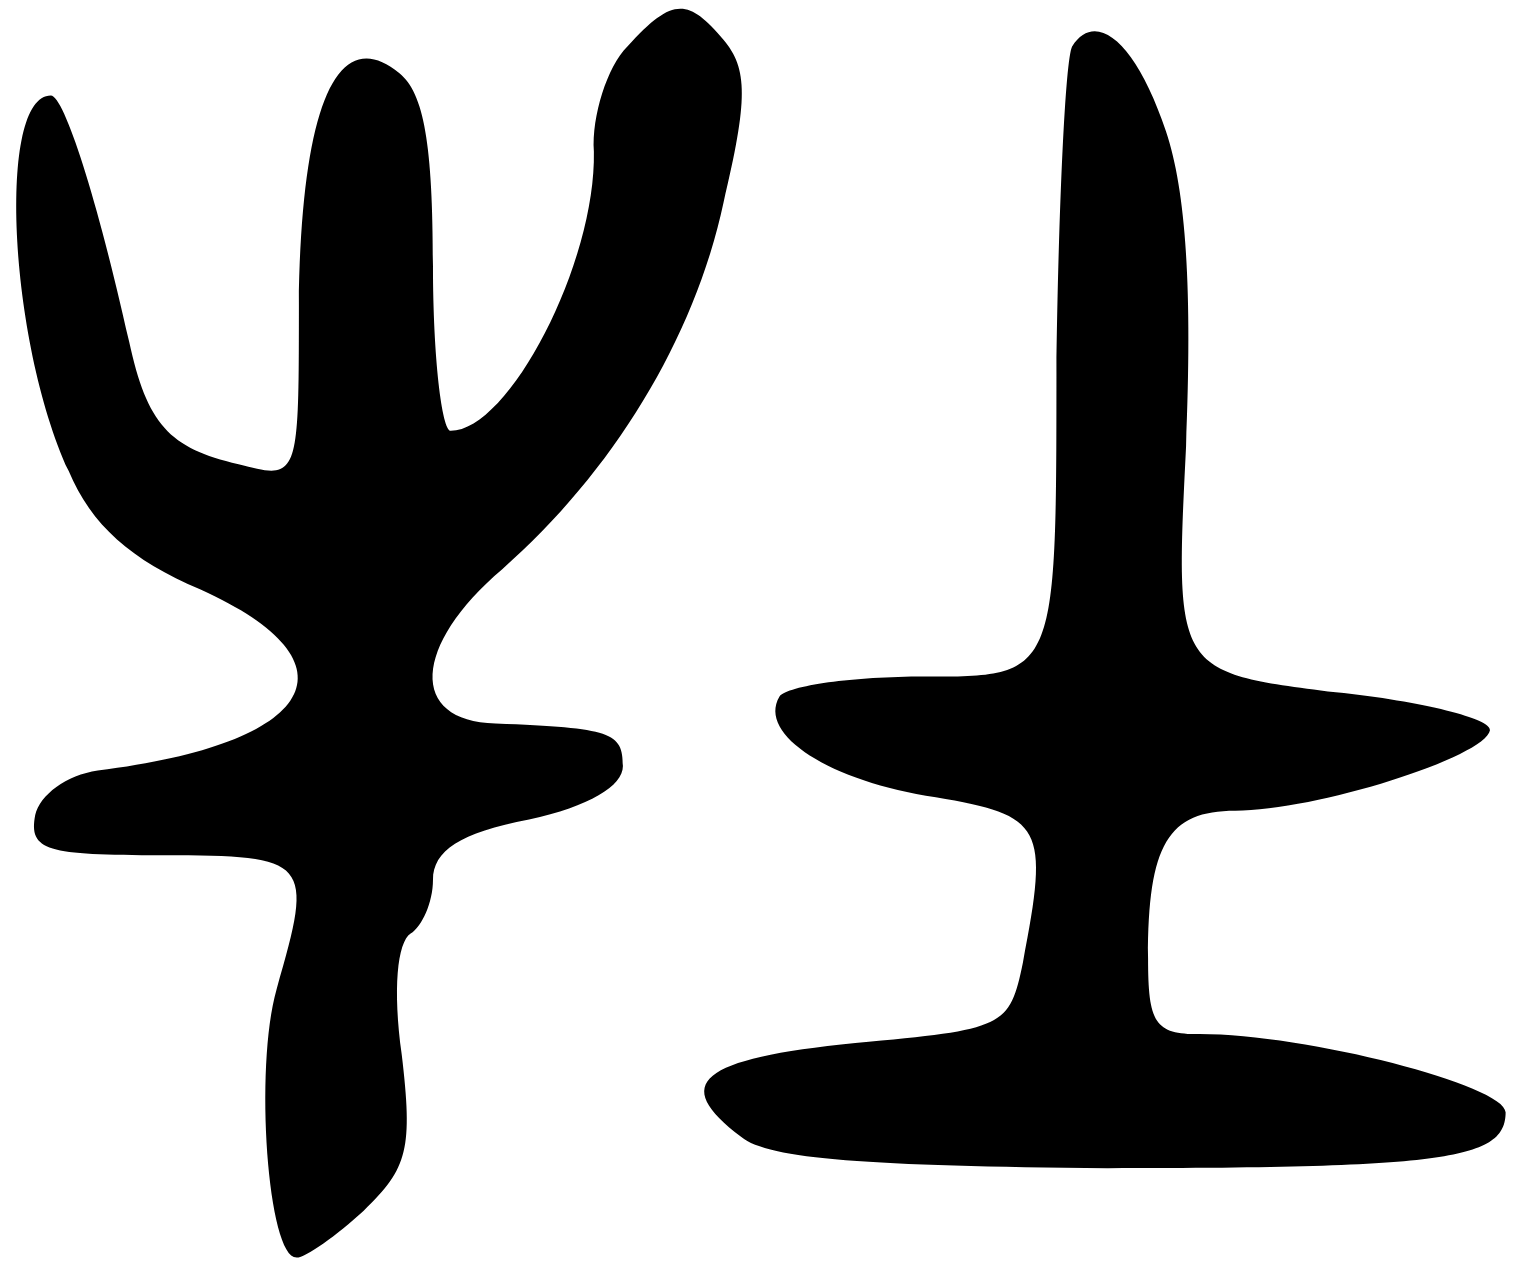
\includegraphics[width=3mm]{Chapter5/dzriX.png} in early texts)
  is historically made up of two semantic components 牛(
\includegraphics[width=2mm]{Chapter5/ngjuw.png} in early texts)
   \emph{ngjuw} `cattle' and 士(
\includegraphics[width=2.5mm]{Chapter5/dzriX2.png}
   in early texts)  \emph{dzriX} `male' and
  altogether lacks a phonetic radical
  \citep[31]{Schuessler2009minimal}. On such
  characters, composed of two or more semantic components without a
  phonetic component (會意 \emph{huìyì}), see 
  \citet[]{Handel2016}.} At the
time of the development of the Chinese script, in order for a character
typically associated with a particular word to serve as a phonetic
indication of a word with an unrelated meaning, the two words must have
been similar in sound. To reconstruct pronunciations at the time of the
script's elaboration it is necessary to have an explicit theory of what
this similarity of sound may have consisted of. Such a theory provides
criteria against which the Middle Chinese pro­nun­ci­a­tions of the two
words in question can be judged similar or dissimilar. Pronunciations
which are dissimilar necessitate explanation in terms of sound change.
This methodology is similar to looking for those cases when a
 \emph{Shījīng} rhyme no longer rhymes in Middle Chinese and then
explaining how the words in question might once have rhymed.

The term 諧聲 `\emph{xiéshēng} series' serves to designate a suite of
characters sharing the same phonetic com­ponent. Zhū Jùnshēng 朱駿聲
(1788-1858) arranged characters by their phonetics in his 說文通訓定聲
 \emph{Shuōwén tōngxùn dìngshēng} (1832). Karlgren produced a similar
work, with the advantage that he provides reference numbers for each
series (1964{[}1957]). Nevertheless, these two works are now outdated;
I instead use the reference numbers from \citet[]{Schuessler2009minimal}.
In some
cases Schuessler thinks that two phonetic series that Karlgren divides
should be united, but he does not implement this unification. For
example, he suggests combining the series built on 屰 \emph{ngjaek}
(02-14) with that built on 朔~ \emph{sraewk} (02-34), but does not
combine the two series in the presentation of his book (2009: 68, 73).
In addition, Baxter \& Sagart propose the unification of some series,
which Schuessler does not accept. For example, Baxter \& Sagart (2014:
143) put 喪  \emph{sang} (03-54a) in the series built on 亡~ \emph{mjang}
(03-65a), but 
\citet[87]{Schuessler2009minimal}
doubts the correctness of this
analysis. Because the present work follows Baxter \& Sagart's
reconstructions, but uses Schuessler's reference numbers, the reader
should be cognizant that the argument at times requires two characters
to be understood as in a single phonetic series despite their reference
numbers implying otherwise.

Duàn Yùcái 段玉裁 (1735-1815) first elaborated the principle, called the
' \emph{xiéshēng} hypothesis', that the same phonetic component in the
writing of two characters implies the words expressed by these
characters have the same rime category in the \emph{Shījīng} (Li 1974:
221).\footnote{The 12th century scholar 徐蕆 Xú Chǎn made a similar
  observation, but less explicitly and less influentially (Behr 2005:
  34).} In other words, characters with the same phonetic component
write words that would have rhymed in the language of the
 \emph{Shījīng}. Li Fang-kuei 李方桂 adds the stipulation that each Old
Chinese rime category have one vowel (Li 1974-5: 243, 
\cite[348]{Baxter1992},
\cite[11]{Schuessler2009minimal}). For words that occur as rhyme words in the
 \emph{Shījīng} and are represented by characters of the same
 \emph{xiéshēng} series, whether or not the readings of these characters
rhyme is a testable hypothesis. There are many such cases. For example,
袺  \emph{ket} \textless{} *{\sil{kˤ}}i{[}t] (29-01q) and 襭  \emph{het}
\textless{} *g{\sil{ˤ}}it (29-01y) rhyme in Ode 8.3 and 脫 \emph{thwajH}
\textless{} *l̥{\sil{ˤ}}ot-s (22-13m) and 帨 \emph{sywejH} \textless{} *l̥ot-s
(22-13g) in Ode 23.3. For characters that do not occur as rhyme words in
the \emph{Shījīng} the \emph{xiéshēng} hypothesis is necessarily an
assumption.

The structure of the Chinese script not only provides a way of
confirming the rime category of words that do not occur as rhyme words
in the \emph{Shījīng} it also provides the primary mechanism for
exploring the initials of Old Chinese, about which the \emph{Shījīng} is
silent. The analogous theory that is used for initials, also called the
' \emph{xiéshēng} hypothesis', is the presumption that all readings in a
single \emph{xiéshēng} series originally began with sounds of the same
place of articulation (Li 1974-5: 228, Baxter 1992: 348, Schuessler
2009: 11).

the \emph{xiéshēng} series built on 皮  \emph{bje} (18-16) illustrates
both the rhyme and the initial facets of the \emph{xiéshēng} hypothesis.

\begin{description} \item
皮  \emph{bje}

\item
被  \emph{bjeX}

\item
陂  \emph{pje}

\item
披  \emph{phje}

\item
跛  \emph{paX}

\item
簸  \emph{paX, paH}

\item
破  \emph{phaH}

\item
婆  \emph{ba}
\end{description}

All Middle Chinese readings in this series have homorganic initials (唇
 \emph{chún} bilabials), and it is reasonable to assume that this state
of affairs is a continuation of what prevailed in Old Chinese. These
readings show two Middle Chinese rimes, -\emph{a} (\emph{gē }歌
 \emph{ka}) and -\emph{je }(\emph{zhī }支  \emph{tsye}). However, words
with these rimes regularly rhyme in the \emph{Shījīng; }for example, 皮
 \emph{bje} rhymes with 紽 \emph{da} in Ode 18.1 and 冝  \emph{ngje}
rhymes with 何 \emph{ha} in Ode 47.1. Noting that in this series the
Middle Chinese rime -\emph{a} (\emph{gē }歌  \emph{ka}) occurs only in
type A words and the Middle Chinese rime -\emph{je} (\emph{zhī }支
 \emph{tsye}) occurs only in type B words, in order to reconcile the
Middle Chinese pronunciations of the series with the \emph{xiéshēng}
hypothesis one could propose that *-a developed to Middle Chinese
-\emph{e} in type B syllables.\footnote{This proposal is valid at the
  level of Han Chinese, but in fact OChi. *-aj \textgreater{} MChi.
  -\emph{a} in type A syllables and MChi. -\emph{e} in type B syllables.
  Final *-j is required for two reasons: 1. to account for
  pronunciations such as Foochow dialect  \emph{muai 2} and Sino-Korean
   \emph{may} for the character 磨 (MChi.  \emph{ma}) (Baxter 1992:
  293-294), 2. to leave OChi. *-a available as an origin of MChi.
  -\emph{u }to explain such phenomena as the early transcription of
  Buddha as 浮屠 (MChi.  \emph{bjuw du}, see Pulleyblank 1983: 78) or
  cognates such as 吾 (MChi. \emph{ngu}) `I, me' compared to Tib. {\tib{ང་
 }} \emph{ṅa} and Bur. {\burm{ငါ}} \emph{ṅā} `id.'.}

In practice, there is seldom need to consult the rhymes of the
 \emph{Shījīng}. Although in some cases the reconstruction of the main
vowel in a \emph{xiéshēng} series is ambiguous if one relies solely on
the Middle Chinese pronunciations of the characters in the series (cf.
§), because Schuessler (2009) takes account of the rhymes of the
 \emph{Shījīng} in his presentation of the \emph{xiéshēng} series, it
generally suffices to consult his work, rather than the poems of the
 \emph{Shījīng} itself. Thus, for example the series built on 欮 (23-11),
containing such Middle Chinese pronunciations as 蕨 \emph{kjwot}, 闕
 \emph{khjwot}, and 橛 \emph{gjwot}, could indicate either *-a- or *-o-
as nuclear vowel. This ambiguity could be resolved by noting that 蕨
 \emph{kjwot} rhymes with 惙 \emph{trjwet} and 說 \emph{ywet} in Ode
14.2; since the latter two Middle Chinese pronunciations descend
unambiguiously from *-o-, it is clear that  \emph{kjwot} must also, but
one need not turn to the Odes since Schuessler resolves the ambiguity
himself by reconstructing 蕨 \emph{kjwot} \textless{} *kot, 闕
 \emph{khjwot} \textless{} *{\sil{kʰ}}ot, 橛  \emph{gjwot} \textless{} *got, etc.
(2009: 240).

\citet[]{Schuessler2009minimal}
does not explicitly distinguish those series which are
in principle reconstructible on the basis of Middle Chinese
pronunciations and the assumption of the \emph{xiéshēng} hypothesis
alone versus those series that require the consultation of the
 \emph{Shījīng} to disambiguate unambiguous reconstruction. In addition,
there is not universal accord on the analysis of rhymes in the
 \emph{Shījīng} and Schuessler does not specify which analysis he relies
upon (see p. n. ). Delicate is the balance between the merits of taking
a few inexplicit decisions on faith versus the merits of doing all the
work again oneself; greater explicitness in future works on Old Chinese
reconstruction is a desideratum.

\subsection{Less traditional sources of data for reconstructing Old
Chinese}\label{less-traditional-sources-of-data-for-reconstructing-old-chinese}

\paragraph{}Baxter \& Sagart additionally
make use of data not normally consulted in the re­con­struction of Old
Chinese, viz. proto-Mǐn (§), early Chinese loan­words into non-Sinitic
languages (§), and morphological spec­u­la­tion (§). For two reasons
separately tracing the epistemo­logical contribution of each these forms
of evidence, working backward from Middle Chinese to the Old Chinese of
their reconstruction, is not currently feasible. First, it is seldom the
case that the evidence of a particular Chinese dialect or a particular
recipient of Chinese loanwords is the sole and unambiguous authority for
a distinction that otherwise there would be no reason to draw; thus,
whereas it is feasible to reconstruct proto-Burmese from Old Burmese
consulting Lashi only to confirm whether a Burmese voiceless aspirate
descends from a plain voiceless or a pre-glottalized obstruent in
proto-Burmish (cf. §), it is not as simple to expand the repertoire of
Old Chinese initials with reference to Mǐn. Second, 
\citet[]{Baxter2014OldChinese}
do not work out the relative chronology of the sound changes they
propose. Until the relative chronology of changes is clarified it will
not be possible to work backward step by step from Middle Chinese to Old
Chinese.

In general, these three less traditional sources of data have no bearing
on either the simplex initials or the rhymes of Old Chinese, but instead
\citet[]{Baxter2014OldChinese}
bring them to bear only with respect to
'pre-initials'. Although the plausibility of `pre-initials' and their
place in Baxter \& Sagart's system are introduced below (§), for the
purposes of introducing the novel types of data that they employ, it is
convenient to preemptively refer to `pre-initials' in this and the
immediately following sections.

\paragraph{proto-Mǐn: } In the study of
Chinese dialects it is traditional to describe a living dialect with
reference to the categories of the  \emph{Qièyùn}. This is an unmotivated
practice, which in a happy development is gradually receding (Norman
2007, Handel 2010). One of the first efforts to show the weakness of the
traditional approach is an influential article by Jerry Norman (1973) in
which he showed that the initial categories of the  \emph{Qièyùn} are
inadequate to predict either initial manner types or tonal developments
in the Mǐn dialects of southern China. For example, Middle Chinese
並~ \emph{b}- corresponds to \emph{p}-,  \emph{p{\sil{ʰ}}}- and \emph{v}- in the
建陽 Kienyang dialect; Norman reconstructs the antecedents of these
segments respectively as *b, *bh, and *‑b in proto-Mǐn (cf. ).\footnote{There
  are some inconsistencies in the data that 
  \citet[]{Norman1973} gives. For
  example, the Amoy word he gives for `thin' appears as pɔˀ 8 on page
  224 but as poˀ 8 on page 227. These inconsistencies do not affect the
  current discussion, but the reader interested in Mǐn should take heed.}
Because of the lenition seen in Kienyang, Norman refers to the proto-Mǐn
segments of the ‑b type as `softened initials' 
\citeyearpar[237]{Norman1973}.
Baxter \&
Sagart use their theory of tightly and loosely attached pre-initials to
account respectively for the voiced aspirated and the softened initials
(\ref{par:reconstructing-tight-pre-initials-using-proto-Min}).

\begin{figure}
    \centering
\begin{tabular}{|l|c|c|c|c|c|c|}
\hline
Middle Chinese &
Proto-Mǐn &
\makecell[c]{Foochow \\
福州}
&
\makecell[c]{Amoy \\
廈門} &
\makecell[c]{Chaochow \\
潮州} &
\makecell[c]{Kienyang \\
建陽} &
\makecell[c]{Kienow \\
建瓯} \\
\hline
白 \textit{baek} 'white' &
*b &
{\sil{pa}} 8 &
{\sil{peˀ}} 8 &
{\sil{peˀ}} 8 &
{\sil{pa}} 8 &
{\sil{pa}} 6
\\ \hline
雹 \textit{baewk} 'hail' &
*bh &
{\sil{p{\sil{ʰ}}oi}} 8 &
{\sil{p{\sil{ʰ}}auˀ}} 8 &
{\sil{p{\sil{ʰ}}ak}} 8 &
{\sil{p{\sil{ʰ}}o}} 8 &
{\sil{p{\sil{ʰ}}au}} 6 \\
\hline
薄 \textit{bak} 'thin' &
*-b &
{\sil{po}} 8 &
{\sil{pɔˀ}} 8 &
{\sil{poˀ}} 8 &
{\sil{vɔ}} 8 &
{\sil{pɔ}} 6 \\
\hline
\end{tabular}
\caption{proto-Mǐn correspondences to Middle Chinese 並 \textit{b}- (after \cite{Norman1973})}
\label{fig:softenedinitials}
\end{figure}

\paragraph{Early Chinese loans into
non-Sinitic languages:} Baxter \& Sagart sporadically employ
comparisons to Sinitic loans in three non-Sinitic families, namely
Vietic, Kra-Dai, and Hmong-Mien. In each case, they understand a
particular feature of a given loanword as requiring explanation as a
reflection of a feature of the donor word, a feature which in many cases
cannot be reconstructed on the basis of Middle Chinese and
 \emph{xiéshēng} evidence.

Fricative initials in Vietnamese sometimes corresponds to a
'pre-syllable' in other Vietic languages, for example Vietnamese
 \emph{va̓i} `cotton',  \emph{vôi} `lime', and \emph{va̓} `hit' have the
Thavung cognates \emph{kpaaś¹}, \emph{ kpuul¹}, and \emph{tpan¹}
respectively (Ferlus 1982: 98); one can thus understand Vietnamese
fricatives as potential evidence of an erstwhile pre-initial. In early
Chinese loans Baxter \& Sagart take Vietnamese spirantization as
evidence of an original Chinese pre-initial 
\citeyearpar[47]{Baxter2014OldChinese}. However,
Vietnamese initial fricatives have multiple origins. Initial \emph{v}-
descends from *w- as well as *Cp- and *Cb-; these two origins are still
distinct in Alexandre de Rhodes' (1651)  \emph{Dictionarium Annamiticum
Lusitanum et Latinum}, the former written  \emph{v}- and the latter
 \emph{ʗb}- 
 \citep[89-90]{Ferlus1982}. To preclude *w- as the source of
 \emph{v}- in any particular word, and thereby secure *Cp- or *Cb- as its
origin, Baxter \& Sagart could have cited the relevant form in de
Rhodes' dictionary. Initial \emph{d}- {[}z] descends from *j- as well
as *Ct- and *Cd- \citep[90]{Ferlus1982}.\footnote{Forms in {[}] reflect the
  pronunciation of Hanoi in our day. 
  \citet[]{Gregerson1969}
  Gregerson (1969: 156) argues that
  Middle Vietnamese \textless{}d-\textgreater{} reflects unlenited /d-/,
  which poses a difficulty for Baxter \& Sagart's analysis. } Ferlus
claims that *j- as an origin of \emph{d- }occurs only in Sino-Vietnamese
words, i.e. a layer of Chinese loans more recent than those which
concern Baxter \& Sagart, but he does not provide an argument on the
basis of tonal correspondences to defend this claim. Initial \emph{r}-
descends from *r- as well as *Cs- and *Cś- 
\citep[91-93]{Ferlus1982}.
%(Ferlus 1982: 91-93). 
Initial
 \emph{gi}- {[}z] (Middle Vietnamese dž-) descends from *kj as well as
*Cč- and *Cǰ- 
\citep[93, 102]{Ferlus1982}.
%(Ferlus 1982: 93, 102). 
Only initial \emph{g}-/ \emph{gh}-
{[}ɣ] uniformly descends from lenited velars 
\citep[91, 99-100]{Ferlus1982}.
%(Ferlus 1982: 91, 99-100). 
Because Vietnamese initial fricatives have multiple origins,
Baxter \& Sagart's use of Vietnamese initial fricatives as \emph{prima
facia} evidence of a lost pre-syllable is not sufficient.

Baxter \& Sagart also cite evidence from other Vietic languages, in
particular Pong, Sách, and Rục. They understand an attested pre-syllable
k- in Rục (e.g. \emph{kəcʌk} `bandit') as evidence that a Chinese donor
word had this same pre-syllable (e.g. 賊  \emph{dzok} \textless{}
*k.dz{\sil{ˤ}}ək {[}05-23a] `bandit')
\citeyearpar[47-48]{Baxter2014OldChinese}.
They take Rục t- as
evidence of Old Chinese *s- 
\citeyearpar[136-137]{Baxter2014OldChinese},
%(2014: 136-137), 
e.g. 肝  \emph{kan
\textless{} }*s.{\sil{kˤ}}a{[}r] (24-01l) `liver' versus Rục \emph{\sil{təkaːn}}
`id.' and 劍 \emph{kjaemH} \textless{} *s.kr{[}a]m-s (36-06i) `sword'
versus Rục \emph{\sil{tə{\sil{kɨ}}əm}} `id.'. Much in developments of presyllables in
Vietic remains shadowy. Nonetheless, the hypothesis of a k- presyllable
continuing unchanged in Rục from the time at which it was borrowed from
Old Chinese (through a line of borrowing which remains to be establish
in detail) is not implausible in view of the remarkable state of
conservation of early phonological oppositions in the Rục language.

For Sinitic loanwords in the Kra-Dai family Baxter \& Sagart make use of
Lakkia, the ``only language in the family that simplifies clusters
having a nasal as their second element by preserving the first consonant
and transferring nasality onto the main vowel'' 
\citeyearpar[36]{Baxter2014OldChinese}. 
The preservation of the cluster initial they use as evidence for *k- and *t-
in Old Chinese, whether tight or loose.

Baxter \& Sagart refer to Chinese loans in proto-Hmong-Mien for evidence
of Chinese *m- or *N- in Old Chinese; in their account these
pre-initials are indistinguishably reflected by pre-nasalization of the
proto-Hmong-Mien initial 
\citeyearpar[48]{Baxter2014OldChinese}.

Aside from the particular reconstructed values Baxter \& Sagart propose,
their reconstruction is an improvement on all others if it captures
systematic relationships among these types of evidence. However, it is
not entirely clear to me that these various types of evidence all point
in the same direction, e.g. that in all cases of a voiced initial in
Middle Chinese corresponding to softened initials in Mǐn the Vietnamese
loan will begin with a fricative and Lakkia and Rục will maintain
pre-initials. Nonetheless, Baxter \& Sagart occasionally do point out
conspiracies of this type. is perhaps their most convincing evidence
that these data systematically correspond 
\citep[37]{Baxter2014OldChinese}.
%(Baxter \& Sagart 2014: 37).

\begin{figure}
    \centering

\begin{tabular}{|l|c|c|c|c|}
\hline
Chinese &
Lakkia &
Vietnamese &
Rục &
proto-Mǐn \\ 
\hline
紙 *k.teʔ > \textit{tsyeX} 'paper' &
khjei 3 &
giấy &
{\sil{kəcáy}} & 
*tš- \\
\hline
賊 *k.dzˤək > \textit{dzok} 'bandit' &
kjak 8 &
giặc &
{\sil{kəcʌ́k}} &
*dzh- \\
\hline
牀 *k.dzraŋ > \textit{dzrjang} 'bed' &
&
&
{\sil{kəc{\sil{ɨ}}ːŋ}} &
*dzh- \\
\hline
箴 *t.[k]əm > \textit{tsyim} 'needle' &
them 1 &
găm &
&
*tš-  \\
\hline
溺 *kə.nˤewk-s > \textit{newH} 'urine' &
kjĩ:w 5 & & & \\
\hline
\end{tabular}
    \caption{Combining the evidence of Kra-Dai, Vietic, and Mǐn}
    \label{fig:combiningKraVieticMin}
\end{figure}

\paragraph{Morphological speculation: }
\label{par:morphological-speculation}
\citet[]{Baxter2014OldChinese} rely on morphological speculation to motivate some
elements of their reconstruction. Their reliance on morphological
conjecture requires some methodological reflection. This method is not
philological, as is the use of  \emph{Shījīng} rhymes or \emph{xiéshēng}
series to modify the internal reconstruction of Middle Chinese. This
method is also not the comparative method, as is the use of proto-Mĭn
data and loans into non-Sinitic languages. The method of adjusting a
proto-language on the basis of morphological speculation is internal
reconstruction. Nonetheless, a distinction must be drawn between
internal reconstruction as used to reconstruct Old Chinese on the basis
of distributional irregularities in Middle Chinese and this internal
reconstruction that makes reference to morphological conjecture. The
former is a method akin to phonemic analysis that relies purely on
phonological distributional patterns, whereas the latter, by making
reference to morphology, necessarily also makes reference to meaning.
Because it relies on meaning, in order to be used in phonetic
reconstruction morphology must be sufficiently clear in a later form of
the language to allow its recognition.

Consideration of both a real and an imaginary instance of internal
reconstruction further brings into focus the methodological issues at
stake. Saussure's formulation of Indo-European laryngeals is the
 \emph{locus classicus} for internal reconstruction.\footnote{Saussure's
  discovery of Indo-European laryngeals was not the first example of the
  method. As early as 1843 in his  \emph{Schulgrammatik} Kühner points to
  the Indo-European \emph{nasalis sonans} with his comment that
  -\emph{n} ``geht bisweilen in 
  {\grk{α}} über'' (p. 17). He points in
  particular to accusative plural -\emph{a} of consonant stems such as {\grk{κόρακα}}
   \emph{kóraka} `raven' (compare -\emph{n} in 
   {\grk{ἵππον}} 
   \emph{híppon}
  `horse') and the third person plural perfect middle ending
  -\emph{atai} as in 
  {\grk{τετάχαται}}  \emph{tetákhatai} `they have been
  arrayed' (compare -\emph{ntai} as in 
  {\grk{ἕστανται}}  \emph{héstantai} `they
  have been stood'). The relevant passage is lacking in the original
  1836 edition of the same work and in his earlier \emph{Ausführliche
  Grammatik} (1834-5). Both Brugmann and Saussure would later claim
  discovery of the \emph{nasalis sonans} (see 
  \cite[133-135]{Joseph2012}, 
  who
  however slightly misstates the bibliographic relationships among
  Kühner's various Greek grammars). Without acknowledging a predecessor,
  \citet[]{Brugmann1876}
    builds his argument on exactly the two environments
  that Kühner drew attention to.} Focussing just on Sanskrit, the root
√yuj (\textless{} IE *i̯eu̯g) `join' has the class VII present
 \emph{yunákti} `joins', with the nasal infix -\emph{ná}-, and the past
participle  \emph{yuktá}- `joined', whereas the root √pū `purify' has the
class IX present \emph{punā́ti} `purify' and the part participle
 \emph{pūtá} `purified'. Saussure realized that the introduction of a
sound change *vH \textgreater{} v̄ allows one to presume that the class
IX presents are ultimately analysable as class VII, i.e. *√puH having
the class VII present *punáHti and the part participle *puHtá \emph{
}(cf. \cite[56]{Clackson2007}).\footnote{In the presentation of this example I
  use modern notation and not that of Sausurre's original (1879).} In
this case the realization that two patterns are sufficiently analogous
to be subsumed as one warrants the presumption of a sound change.
Because none of the uses to which Baxter \& Sagart put morphological
conjecture in the service of phonological reconstruction is parallel
with this case, I have invented a scenario in English that has a
structure more parallel to their method.

The first step is to identify something in a synchronic system that
looks like (possibly defunct) morphology. Good candidates are typically
what Matisoff would call an `allofam', i.e. words that share both a
phonetic and semantic similarity 
(cf. \cite{Matisoff1978}). Consider
 \emph{drink} and \emph{drench}. The next step is to search for other
examples of the pattern. This search requires as explicit as possible
description of both the phonology and the semantics of the pattern, even
if the pattern requires some speculation, for example the interpretation
of \emph{drench} as `make drink'. The search turns up
 \emph{rise}/\emph{raise},  \emph{lie}/\emph{lay},  \emph{sit}/\emph{set},
and \emph{fall}/\emph{fell}. In each case there is a pair of verbs, a
non-causative and a causative; the non-causative is strong and the
causative is weak. Since strong verbs are inherited, and would be
presumed to be inherited even in ignorance of the history of English, it
is judicious to derive the causative from the non-causative. The
causative always has vowel -\emph{e}- or diphthong -\emph{ai}- and
palatalises the -\emph{k} of \emph{drink}. If one assumes that
non-segmental alternations of this kind arise from segmental sources it
is possible to postulate something like an *-e- causative suffix. With
this hypothesis in hand, one may explore the interaction of this
hypothesis with the overall set of stable hypotheses about the history
of English.

This methodology is more convincing when the meaning of the
morpho­logical alternation in question is supported with philological
evidence from as early of texts as possible. Unfortunately, in current
practice morphological alternations are usually argued for on the basis
of dictionary definitions and are seldom exhibited with textual
attestations. Until the philology is there to back up the reality of the
morphological analysis, the use of morpho­logical speculation in the
phonetic reconstruction of Chinese should be treated with great
caution.\footnote{Morphological speculation is most convincing when
  presented in a comparative context. For example, the causative
  formation of English \emph{drink}/\emph{drench} is much clearer in the
  Gothic pairs \emph{drigkan}/\emph{dragkjan},
   \emph{urreisan}/\emph{urraisjan},  \emph{ligan}/\emph{lagjan},
   \emph{sitan}/\emph{satjan}, and is clearer still in Sanskrit
   \emph{sī́dati} \textless{} *sísdeti versus \emph{sādáyati} \textless{}
  *sodéi̯eti (cf.
  \cite[98 §5.32]{Fortson2010}). The comparative
  con­tex­tu­aliza­tion of Chinese historical morphology is almost
  entirely absent.}

Some of Baxter \& Sagart's morphological speculations are more
convincing than others. The clearest case is a voicing alternation
between transitive and intransitive verbs in Middle Chinese (§). Rather
less obvious are prefixes such as *m{\sil{₂}}- in body parts and *m₃- in animal
names 
\citeyearpar[55-56]{Baxter2014OldChinese}.\footnote{In support of the reconstruction of an m-
  `animal prefix' Sagart cites the modern Mandarin forms 螞蚱
   \emph{màzhà} `grasshopper', 馬蜂  \emph{mǎféng} `hornet', 螞蝗
   \emph{mǎhuáng} `leech', and 螞蟻  \emph{mǎyǐ} `ant', Fuzhou  \emph{{\sil{ma₃₁}}}
   \emph{{\sil{u₅₂}}} `dragonfly', Guangzhou  \emph{{\sil{ma₂₃ khɔŋ₂₁ lɔŋ₂₁}}} `praying
  mantis', Bao'an Cantonese  \emph{{\sil{ma₂₁ tsɐu₅₅ sy₁₁}}} `bat', and Gongha
  Hakka \emph{{\sil{ma₄₄ sam₃₅}}} `cicada' 
  \citeyearpar[85]{Sagart1999}.} The English words
'head', `heel', `heart', and `hand' all begin with `h', but English is
not conventionally described as having an `h' prefix in these words. The
Latin words for domesticated animals  \emph{cattus} `cat',
 \emph{caballus} `horse',  \emph{capra} `goat', and \emph{camelus} `camel'
all begin with \emph{ca}-, but this syllable is not normally reckoned an
'animal prefix' (Hill 2014 `derivation' : 629-630 also cf. §d and
§b).
%\footnote{I thank Arnaud Fournet for drawing my attention to these Latin examples (\emph{per litteras} 10 February 2017).} 
Of course, a
morpheme is nothing more than a conventional as­so­ci­a­tion of form and
meaning 
\citep[65-76]{Hockett1987refurbishing}.
%(Hockett 1987: 65-76). 
Just as the association of `h' with body
parts in English or \emph{ca}- with domesticated animals in Latin are
available to any listener; the associations of form and meaning that
Baxter \& Sagart index with these prefixes are there to be observed, but
whether native hearers of Old Chinese understood them as prefixes and
whether they continue inherited material also bequeathed to other
languages are both difficult questions to answer.

\section{Simplex initials of Old
Chinese}

\paragraph{}
\label{par:lex-initials-of-old-chinese}
Reconstruction of the simplex initials of Old Chinese can be
conceptualized as proceeding in two steps. An internal re­con­struction
of Middle Chinese serves as the first step (§§-). As a second step
 \emph{xiéshēng} contacts provide motivation for further hypotheses
(§§-). Internal re­con­struction tends to reduce the number of initials.
The resultant simpler inventory of initials tidies up the
 \emph{xiéshēng} series and brings violations of the \emph{xiéshēng}
hypothesis into sharper focus. Suggesting explanations for these
apparent violations again expands the number of initials.

\subsection{Internal reconstruction of Middle Chinese
initials}\label{internal-reconstruction-of-middle-chinese-initials}

\paragraph{} Patterns of complementary distribution in Middle Chinese allow one to
suggest that multiple Middle Chinese initials arose as conditioned
variants of the same Old Chinese initial. Making use of the patterns of
complementary distribution one can preclude the existence in Old Chinese
of \emph{h}- (匣 \emph{xiá}) (§), the palatal affricates (\emph{zhāngzǔ}
章組 \emph{Tsy}-) (§),  \emph{l}- (來  \emph{lái}), the retroflex stops
(\emph{shéshǎng} 舌上  \emph{Tr}-), and the retroflex affricates
(\emph{zhuāngzǔ~}莊組 \emph{Tsr}-) (§). Internal re­con­struc­tion also
permits the postulation of a series of initial labiovelars and
provisionally labio-glottals (§). presents the initials of Old Chinese
to the extent that they can be recovered on the basis of the internal
reconstruction of Middle Chinese.

\paragraph{Origin of Middle Chinese 匣 \emph{\textbf{h}}-}. Middle
Chinese initial \emph{h}- (匣 \emph{xiá}) is in complementary
dis­tri­bu­tion with Middle Chinese \emph{g}- (群  \emph{qún}). Initial
 \emph{g}- only occurs in type B syllables whereas \emph{h}- only occurs
in type A syllables (Schuessler 2009: 13, cf. ). As Karlgren suggests
(1923: 21-22), this distribution allows one to assume that Old Chinese
had no *h-, and that there was a regular change *g- \textgreater{} 匣
 \emph{h}- in type A syllables.

\begin{figure}
    \centering
\begin{tabular}{|c|c|c|}
\hline
&
Type A &
Type B \\
\hline
見 k- &
干 kan &
建 kjonH \\
\hline
溪 kh- &
看 khanH &
褰 khjen \\
\hline
群 g- &
--- &
乾 gjen \\
\hline
匣 h- &
寒 han &
--- \\
\hline
\end{tabular}
    \caption{The Middle Chinese complementary distribution 
of 群 \textit{g-} and 匣 \textit{h-} (after \cite{Schuessler2009minimal})}
    \label{fig:HandG}
\end{figure}

\paragraph{Origin of palatal
affricates.} Whereas dental initials (端 \emph{t}-, 透
 \emph{th}-, 定 \emph{d}-) occur only with type A rimes, palatal
affricates (章 \emph{tsy}-, 昌 \emph{tsyh}-, 船 \emph{zy}-) occur only
with type B rimes. As Karlgren notes (1923: 24), this complementary
distribution allows for the interpretation that the palatal affricates
in type B rimes developed from dentals (端  \emph{t}- \textless{} *t{\sil{ˤ}}-,
章  \emph{tsy}- \textless{} *t-, etc.) 
\citep[12]{Schuessler2009minimal}.

\paragraph{Origin of 來
 \emph{l}- and the retroflex consonants.}
No type A
rimes with the main vowels -\emph{ae}- and -\emph{ea}- (division-ii)
occur with dental initials (\emph{shétóu} 舌頭  \emph{T}-) and only very
rarely with initial 來 \emph{l}-. No type A rimes with the main vowels
-\emph{a}-, -\emph{o}-, -\emph{u}-, or -\emph{e}- (division-i/iv) occurs
with retroflex stops (\emph{shéshǎng} 舌上  \emph{Tr}-). Noting this
com­ple­men­tary distribution of the initials and main vowels, Jaxontov
proposed that the dental and retroflex initial classes were originally
the same (1960a: 2-9, also see 
\cite[262-267]{Baxter1992}).\footnote{Jaxontov
  originally proposed medial -l-, but subsequent researchers have
  generally amended this to -r- (see 
  \cite[262]{Baxter1992}). On the basis of
  \emph{xiéshēng} connections between initial 來 \emph{l}- and velars
  von der Gabelentz similarly proposed clusters such as *kl- (1881: 99,
  §223). } Noting that ty­po­lo­gi­cal­ly a medial -\emph{r}- is known
to give rise both to \emph{l}- and to retroflex initials (e.g. *dr-
\textgreater{} ʈ- in Lhasa Tibetan, cf. 

\citet[388]{Tournadre2009manuel},
*r- \textgreater{} l- in Classical Sanskrit, cf. 
\cite[204 §10.8, 211 §10.34]{Fortson2010}), it is reasonable to conjecture that Middle Chinese
initial 來 \emph{l}- was initial *r- in Old Chinese and that Middle
Chinese retroflex initials derive from Old Chinese dental initials
followed by medial -r- (知 \emph{tr}- [{\sil{ʈ}}] \textless{} *tr- etc.).
Similar considerations lead to the conclusion that the retroflex
affricates (\emph{zhuāngzǔ~} 莊組 \emph{Tsr}-) originate from affricates
followed by a medial -r- (cf. 
\cite[203-206]{Baxter1992}).\footnote{Han
  dynasty Buddhist transcriptions of Sanskrit r- with MChi. initial 來
   \emph{l}- may reinforce the impression that the ancestor of this
  segment was pronounced as r- at the time of the transcription, e.g.
  Skt. \emph{saṃghārāma} 僧伽藍 \emph{song gja lam}, Skt. \emph{arhat}
  阿羅漢 \emph{'a la xanH}, Skt.  \emph{anuttarā}- 阿耨多羅 \emph{'a nuwH
  ta la}, Skt. \emph{pāramitā} 波羅蜜 \emph{pa la mjit}, Skt.
   \emph{śarīra}舍利 \emph{syaeX lijH}. However, since inherited *l- (cf.
  §) was lost before the encounter with Buddhism, this evidence does not
  support the reconstruction of the ancestor of MChi. 來  \emph{l}- as
  *r- in contrast to *l-.}

\begin{figure}[t]
    \centering

\begin{tabular}{|lllllll|}
\hline
 Plain (type B): &
*{\sil{p-}} &
*{\sil{p{\sil{ʰ}}-}} &
*{\sil{b-}} &
*{\sil{m-}} &
&
\\
&
*{\sil{t-}} &
*{\sil{t{\sil{ʰ}}-}} &
*{\sil{d-}} &
*{\sil{n-}} &
&
\\
&
*{\sil{ts-}} &
*{\sil{ts{\sil{ʰ}}-}} &
*{\sil{dz-}} &
&
*{\sil{s-}} &
*{\sil{z-}} \\
&
*{\sil{k-}} &
*{\sil{{\sil{kʰ}}-}} &
*{\sil{g-}} &
*{\sil{ŋ-}} &
&
\\
&
*{\sil{{\sil{kʷ}}-}} &
*{\sil{{\sil{kʰ}}{\sil{ʷ}}-}} &
*{\sil{g{\sil{ʷ}}-}} &
*{\sil{ŋ{\sil{ʷ}}-}} & 
&
\\
&
*{\sil{ʔ-}} &
&
&
&
*{\sil{x-}} &
\\&
*{\sil{ʔ{\sil{ʷ}}-}} &
&
&
&
*{\sil{x{\sil{ʷ}}-}} &
\\ 
&
*{\sil{r-}} &
&
*{\sil{hj-}} & 
&
&
\\
&&&
*y- &
&
&
\\
Pharyngealized (type A): &
*{\sil{pˤ-}} &
*{\sil{p{\sil{ʰ}}ˤ-}} &
*{\sil{bˤ-}} &
*{\sil{mˤ-}} &
&
\\&
*{\sil{tˤ-}} &
*{\sil{t{\sil{ʰ}}ˤ-}} &
*{\sil{dˤ-}} &
*{\sil{nˤ-}} &
&
\\&
*{\sil{tsˤ-}} &
*{\sil{ts{\sil{ʰ}}ˤ-}} &
*{\sil{dzˤ-}} &
&
*{\sil{sˤ-}} &
*{\sil{zˤ-}} \\
&
*{\sil{kˤ-}} &
*{\sil{{\sil{kʰ}}ˤ-}} &
*{\sil{gˤ-}} &
*{\sil{ŋˤ-}} &
&
\\&
*{\sil{{\sil{kʷ}}ˤ-}} &
*{\sil{{\sil{kʰ}}{\sil{ʷ}}ˤ-}} &
*{\sil{g{\sil{ʷ}}ˤ-}} &
*{\sil{ŋ{\sil{ʷ}}ˤ-}} &&
\\&
*{\sil{ʔˤ-}} &
&
&
&
*{\sil{xˤ-}} &
\\&
*{\sil{ʔ{\sil{ʷ}}ˤ-}} &
&
&
&
*{\sil{x{\sil{ʷ}}ˤ-}} &
\\&


*{\sil{rˤ-}} &
&
*{\sil{hjˤ-}} &
&
&
\\
&&&
*{\sil{yˤ-}} &&& \\
\hline
\end{tabular}

    \caption{Old Chinese initials on the basis of Middle Chinese internal reconstruction}
    \label{fig:OChionMChi}
\end{figure}


\paragraph{Old Chinese
labio-velars.} Middle Chinese syllables with medial -\emph{w}- (合口
 \emph{hékǒu}) fall neatly into two categories. The first category
consists of syllables with checked rimes that occur only after velars
(牙 \emph{yá}) or glottals (喉  \emph{hóu}). This category includes such
Middle Chinese rimes as \emph{táng / yáng} 唐阳 -\emph{wang} /
‑ \emph{jwang},  \emph{dēng} 登 \emph{-wong},  \emph{gēng-èr} 庚二
-\emph{waeng},  \emph{gēng} 耕 -\emph{weang}, and \emph{xiān} 先
-\emph{wen}). Thus, there are no Middle Chinese syllables of the type
*trwaeng, *tswen, *lwong or *dwang. The second category includes all
other rimes (‑ \emph{win}, ‑ \emph{won}, etc.), which appear freely with
all initials. This constrained distribution of medial -\emph{w}- in
Middle Chinese suggests that Old Chinese had no freely occurring medial
-\emph{w}-; these two distributional classes imply two separate origins
for -\emph{w}-. One source of -\emph{w}- (-*w{\sil{₁}}-) arose only after velars
and glottals but could occur in any rime, whereas another source of
-\emph{w}- (-*w{\sil{₂}}-) arose in certain rimes, but could occur with any
initial. After velars and glottals the outcome of these two sources are
conflated in those rhymes that do not require velar and glottal initials
(i.e. *kw{\sil{₁}}ang, *kw{\sil{₁}}in, *kw{\sil{₂}}in, *tw{\sil{₂}}in \textgreater{} \emph{kwang, kwin,
twin}). 
\citet[359]{Haudricourt1954b}\footnote{See also Jaxontov 1960b: 104, 1970: 54.}
explains the origin of -*w{\sil{₁}}- by positing the former existence of unitary
labiovelar consonants, e.g. 光 \emph{kwang} \textless{} *{\sil{kʷˤ}}aŋ (03-22a),
壙 \emph{khwangH} \textless{} *{\sil{k{\sil{ʷʰ}}ˤ}}aŋ-s (03-23n), etc. (cf. \cite[214-218]{Baxter1992}). For the moment one may presume the existence of labio-glottals
also (e.g. 枉 \emph{'jwangX} \textless{} *ʔ{\sil{ʷ}}aŋʔ {[}03-26q], 汪
 \emph{'wang} \textless{} *{\sil{ʔ{\sil{ʷ}}ˤ}}aŋ {[}03-26r]. etc.), but on the basis of
 \emph{xiéshēng} evidence these are better reconstructed as labio-uvulars
(cf. §). For the origin of the Middle Chinese medial -\emph{w}- that is
not restricted as to its co-occurence with class of initial (*-w{\sil{₂}}-) see \ref{par:rounded-vowel}.

\subsection{\texorpdfstring{Expanding the Old Chinese initials using
 \emph{xiéshēng}
evidence}{Expanding the Old Chinese initials using xiéshēng evidence}}\label{expanding-the-old-chinese-initials-using-xiuxe9shux113ng-evidence}

\paragraph{}. According to the \emph{xiéshēng}
hypothesis, in a given phonetic series only initials from the same point
of articulation occur (Li 1974-5: 228,
\cite[11]{Schuessler2009minimal}
cf. §). All
those  \emph{xiéshēng} series which mix Middle Chinese pronunciations
with non-homorganic initials provide an opportunity to explain the
divergent Middle Chinese pronunciations as phonetically conditioned
developments of Old Chinese readings with homorganic initials.

\paragraph{Laterals}. Some \emph{xiéshēng}
series, such as the series built on 它 (18-09), present character
readings with Middle Chinese initials 以  \emph{y}-, 定~ \emph{d}- and 澄
 \emph{dr}-. In such series, 定  \emph{d}- is always found in type A
syllables and 以 \emph{y}- in type B syllables. Following a suggestion
of Pulleyblank (1973: 117-118), Baxter \& Sagart understand
 \emph{xiéshēng} series of this type as originally having lateral
initials in all cases 
\citep[109]{Baxter2014OldChinese}, suggesting the sound changes *l-
\textgreater{} 以  \emph{y}-, *l({\sil{ˤ}})r- \textgreater{} 澄  \emph{dr}-, and
*l{\sil{ˤ}}- \textgreater{} 定  \emph{d}-.

\begin{description} \item
也  \emph{yaeX} \textless{} *l- (18-09g)

\item
池  \emph{drje} \textless{} *lr- (18-09t)

\item
地  \emph{dijH} \textless{} *l{\sil{ˤ}}- (18-09b')
\end{description}

As confirmation of the lateral origins of initials in such series Baxter
\& Sagart draw attention to the preservation of lateral initials in the
瓦鄉 Wǎxiāng and 閩 Mǐn dialects as well as in loanwords into Vietnamese
and Hmong-mien 
\citeyearpar[109-110]{Baxter2014OldChinese}, e.g. 地  \emph{dijH} \textless{} *l{\sil{ˤ}}-
(18-09b') `earth, ground' pronounced /li 22/ in the Wǎxiāng dialect
Gǔzhàng.

\paragraph{Voiceless resonants}. In some
 \emph{xiéshēng} series with predominantly voiced resonant initial
readings, the occasional character instead has a reading with a
voiceless obstruent initial. Dǒng Tónghé 董同龢 posited a voiceless
labial nasal to explain the voiceless obstruent initial readings in
series with predominantly bilabial nasal initial readings (1949: 12-14).
Pulleyblank extended the proposal to the velar, labio-velar, and dental
nasals and the voiceless lateral (1962: 92, 121, 141). Baxter adds the
voiceless rhotic 
\citep[201-202]{Baxter1992}. Baxter \& Sagart accept these previous
proposals 
\citeyearpar[111-116]{Baxter2014OldChinese}.

§a. The voiceless velar nasal develops to 曉  \emph{x}- in both type A
and type B syllables. The series built on ⼚ (24-15) furnishes evidence
for the reconstruction of a type A voiceless velar nasal and the change
*ŋ̊{\sil{ˤ}}- \textgreater{} 曉 \emph{x}-.

\begin{description} \item
⼚  \emph{xanX} \textless{} *ŋ̊{\sil{ˤ}}- (24-15a)
\item
雁  \emph{ngaenH} \textless{} *ŋ- (24-15b)
\end{description}

The series built on 我 (18-05) furnishes evidence for the reconstruction
of a type B voiceless velar nasal and the change *ŋ̊- \textgreater{} 曉
 \emph{x}-.

\begin{description} \item
我  \emph{ngaX} \textless{} *ŋ{\sil{ˤ}}- (18-05a)
\item
儀  \emph{ngje} \textless{} *ŋ- (18-05u)
\item
犧  \emph{xje} \textless{} *ŋ̊- (18-05z)
\end{description}

§b. The voiceless labial nasal develops to 曉  \emph{x}- in both type A
and type B syllables. The series built on 黑 (05-38) furnishes evidence
for the reconstruction of a type A voiceless labial nasal and the change
*m̥{\sil{ˤ}}- \textgreater{} 曉 \emph{x}-.

\begin{description} \item
黑  \emph{xok} \textless{} *m̥{\sil{ˤ}}- (05-38a)
\item
墨 \emph{mok} \textless{} *m{\sil{ˤ}}- (05-38c)
\end{description}

The series built on 烕 (20-19) furnishes evidence for the reconstruction
of a type B voiceless dental nasal and the change {\sil{*m̥-}} \textgreater{} 曉
 \emph{x}-.

\begin{description} \item
烕  \emph{xjwiet} \textless{} {\sil{*m̥-}} (20-19a)
\item
滅 \emph{mjiet} \textless{} *m- (20-19b)
\end{description}

§c. The voiceless dental nasal behaves differently in type A and type B
syllables. The series built on 嘆 (24-35) furnishes evidence for the
reconstruction of a type A voiceless dental nasal and the change *{\sil{n̥ˤ}}-
\textgreater{} 透  \emph{th}- (cf. 
\cite[193]{Baxter1992}).

\begin{description} \item
嘆  \emph{than} \textless{} *{\sil{n̥ˤ}}- (24-35a)
\item
難  \emph{nan} \textless{} *n{\sil{ˤ}}- (24-35d)
\item
㸐  \emph{nyen} \textless{} *n- (24-35i)
\end{description}

The series built on 女 (01-56) furnishes evidence for the reconstruction
of a type B voiceless dental nasal and the change *n̥- \textgreater{} 書
 \emph{sy}- (cf. Baxter 1992: 194).

\begin{description} \item
女  \emph{nrjoX} \textless{} *nr- (01-56a)

\item
如  \emph{nyo} \textless{} *n- (01-56g)

\item
恕  \emph{syoH} \textless{} *n̥- (01-56t)
\end{description}

The series built on 耳 (04-40) furnishes evidence for the reconstruction
of a type B voiceless dental nasal with medial -r- and the change *n̥r-
\textgreater{} 徹~ \emph{trh}- (cf. 
\cite[195-196]{Baxter1992}).

\begin{description} \item
耳  \emph{nyiX} \textless{} *n- (04-40/0981a)

\item
恥  \emph{trhiX} \textless{} *n̥r- (04-40/0959a)
\end{description}

§d. The voiceless lateral develops differently in type A and type B
syllables. The series built on 俞 (10-23) furnishes evidence both for
the reconstruction of a type A voiceless lateral and the sound changes
*l̥{\sil{ˤ}}- \textgreater{} 透 \emph{th}- and the reconstruction of a type B
voiceless lateral and the sound change *l̥- \textgreater{} 書  \emph{sy}-.

\begin{description} \item
俞  \emph{yu} \textless{} *l- (10-23a)

\item
歈  \emph{duw} \textless{} *l{\sil{ˤ}}- (10-23t)

\item
輸  \emph{syu} \textless{} *l̥- (10-23s)

\item
偷  \emph{thuw} \textless{} *l̥{\sil{ˤ}}- (10-23u)
\end{description}

§e. The voiceless rhotic develops differently in type A and type B
syllables. The series built on 豊 (26-23) furnishes evidence for the
reconstruction of a type A voiceless rhotic and the sound change *r̥{\sil{ˤ}}-
\textgreater{} 透  \emph{th}-.

\begin{description} \item
豊  \emph{lejX} \textless{} *r{\sil{ˤ}}- (26-23a)

\item
禮  \emph{lejX} \textless{} *r{\sil{ˤ}}- (26-23d)

\item
體  \emph{thejX} \textless{} *r̥{\sil{ˤ}}- (26-23i)
\end{description}

The series built on �� (01-51) furnishes evidence for the reconstruction
of a type B voiceless rhotic and the sound change *r̥- \textgreater{} 徹
 \emph{trh}-.

\begin{description} \item
�� \emph{lu} \textless{} *r{\sil{ˤ}}- (01-51a)

\item
鑪  \emph{lu }\textless{} *r{\sil{ˤ}}- (01-51m)

\item
廬  \emph{ljo} \textless{} *r- (01-51q)

\item
攄  \emph{trhjo} \textless{} *r̥- (01-51x)
\end{description}

\begin{figure}
    \centering
\begin{tabular}{|c|c|c|c|}
\hline
\multicolumn{2}{|c}{Type A} &
\multicolumn{2}{c|}{Type B} \\
\hline
OChi. &
MChi. &
OChi. & 
MChi. \\
\hline
*{\sil{ŋ̊ˤ-}} > &
\multirow{2}{*}{曉 {\emph{x-}}}
%曉 x- 
&
*{\sil{ŋ̊-}} > &
\multirow{2}{*}{曉 {\emph{x-}}}
% 曉 x- 
\\ 
{\sil{*m̥ˤ}}- > &
&
*{\sil{m̥-}} > &
\\ \cline{2-2} \cline{4-4}
%\hline
*{\sil{n̥ˤ-}} > &
\multirow{3}{*}{透 {\emph{th-}}}
&
*{\sil{n̥-}} > &\multirow{2}{*}{書 {\emph{sy}}-} \\ 
{\sil{*l̥ˤ-}} > &
&
*{\sil{l̥-}} >% &
&
\\ \cline{4-4}
*{\sil{r̥ˤ-}} > &
&
*{\sil{r̥-}} >  &
徹 
{\emph{trh-}} 
\\ 
\hline
\end{tabular}

%\end{tabular}
    \caption{The development of Old Chinese voiceless resonants in Middle Chinese}
    \label{fig:OChivcresonants}
\end{figure}

summarizes the development of Old Chinese voiceless resonants in Middle
Chinese (cf. \cite[112]{Baxter2014OldChinese}).\footnote{Baxter \& Sagart also
  present evidence that a western dialect of early Chinese instead
  underwent the changes *n̥({\sil{ˤ}})- , *l̥({\sil{ˤ}})- \textgreater{} 曉  \emph{x}-
  (2014: 112-114). The examples Baxter \& Sagart discuss include
  initials *{\sil{n̥ˤ}}- (type A), *l̥{\sil{ˤ}}- (type A), and *l̥- (type B), i.e. they do
  not give an example of *n̥- (type B) \textgreater{} 曉  \emph{x}-. They
  also make no comment above the development of *r̥({\sil{ˤ}})- in this western
  dialect.}

\paragraph{Uvulars.} Some  \emph{xiéshēng}
series mix readings with Middle Chinese velars (見  \emph{k}-, 群
 \emph{g}-, 匣~ \emph{h}-, 曉  \emph{x}-) and readings with initial glottal
stop (影 `-) or initial 以  \emph{y}-. Following a proposal of Pan
(1997), Baxter \& Sagart propose that the fricative (匣  \emph{h}-, 曉
 \emph{x}-), glottal (影 `-) and glide (以  \emph{y}-) initials found in
such series originate from uvular initials (2014: 43-46, also cf. 
Sagart
\& Baxter 2009).\footnote{It is also possible to reconstruct a series
  with only Middle Chinese velar initials as uvular, if it contains some
  readings that begin with 曉  \emph{x}- (cf. §). } Their explanation for
the velar stops (見  \emph{k}-, 群  \emph{g}-) occurring in the relevant
series are discussed below (§). In support of the uvular hypothesis one
can mention Vovin's comparison of the titles for foreigner dignitaries
attested in the early Han period 護于  \emph{huH hju} \textless{}
*{\sil{[ɢ]ʷˤ}}ak-s *{\sil{ɢʷ}}(r)a (02-08k, 01-23a), which he sees as a
transcription of proto-Yeniseian *{\sil{qaʔ-ɢā}} `great ruler', and 單于
 \emph{dzyen hju} \textless{} *dar *{\sil{ɢʷ}}(r)a (24-21a, 01-23a) which he
compares to Old Turkic \emph{tarqan} (Vovin 2007: 180).

§a. The series built on 匃 (21-01) furnishes evidence for the
reconstruction of voiceless, voiceless aspirated, and voiced uvulars and
the changes *q- \textgreater{} 影 `-, {\sil{*qʰ}}- \textgreater{} 曉  \emph{x}-,
*{\sil{ɢ}}- \textgreater{} 匣 \emph{h}-.

\begin{description} \item
匃  \emph{kat} (21-01a)

\item
謁  \emph{'jot} \textless{} *q- (21-01x)

\item
歇  \emph{xjot} \textless{} {\sil{*qʰ}}- (21-01u)

\item
褐 \emph{hat} \textless{} *{\sil{ɢˤ}}- (21-01g)
\end{description}

§b. Baxter \& Sagart restrict the change *{\sil{ɢ}}- \textgreater{} 匣 \emph{h}-
to type A syllables; doing so makes *{\sil{ɢ}}- in type B syllables available as
an origin of 以 \emph{y}- in a series such as that built on 衍 (24-29).

\begin{description} \item
衍  \emph{yenH} \textless{} *{\sil{ɢ}}- (24-29a)

\item
愆  \emph{khjen} (24-29b)

\item
餰 \emph{khjen} (24-29c)
\end{description}

Baxter \& Sagart do not posit an initial *j- in Old Chinese; they take
*l- (cf. §) and *{\sil{ɢ}}- (or *{\sil{ɢʷ}}-, cf. §d), and pre-initials before *r- (cf.
§b), as the only three sources of Middle Chinese 以~ \emph{y}-.

§c. Baxter \& Baxter derive the Middle Chinese initial 云 \emph{hj}-
uniformly from Old Chinese *{\sil{ɢʷ}}- in type B syllables (Sagart \& Baxter
2009: 233-234). This hypothesis accounts for the distribution of initial
云 \emph{hj}- to (nearly) exclusively type B syllables with medial
-\emph{w}- 
\citep[209]{Baxter1992}. The series built on 王 (03-26) furnishes
evidence for the reconstruction of the voiced labio-uvular stop in type
B syllables, along with the change *{\sil{ɢʷ}}- \textgreater{} 云~ \emph{hj}-.

\begin{description} \item
王  \emph{hjwang} \textless{} *{\sil{ɢʷ}}- (03-26a)
\item
匡  \emph{khjwang} (03-26m)
\item
狂  \emph{gjwang} (03-26o)
\item
枉  \emph{'jwangX} \textless{} {\sil{*qʷ}}- (03-26q)
\item
汪  \emph{'wang} \textless{} {\sil{*qʷˤ}}- (03-26r)
\end{description}

The series built on 于 (01-23) also supports the proposal *{\sil{ɢʷ}}-
\textgreater{} 云  \emph{hj}-.

\begin{description} \item
于 \emph{hju} \textless{} *{\sil{ɢʷ}}(r)- (01-23a)
\item
污  \emph{'wae} \textless{} {\sil{*qʷˤ}}r- (01-23c')
\item
訏 \emph{xju} \textless{} {\sil{*qʷʰ}}(r)- (01-23v)
\end{description}


§d. At first glance a series such as that based on 肙 (23-17) appears to
point instead to the proposal *{\sil{ɢʷ}}-\textgreater{} 以  \emph{y}-.

\begin{description} \item
肙  \emph{'wen} \textless{} {\sil{*qʷˤ}}- (23-17a)
\item
駽  \emph{xwen} \textless{} {\sil{*{\sil{qʷʰ}}ˤ}}- (23-17k)
\item
捐  \emph{ywen} \textless{} *{\sil{ɢʷ}}- (23-17g)
\item
鞙  \emph{hwenX} \textless{} *{\sil{ɢʷˤ}}- (23-17j)
\end{description}

However, the two proposals *{\sil{ɢʷ}}- \textgreater{} 云  \emph{hj}-\emph{ }and
*{\sil{ɢʷ}}-\textgreater{} 以  \emph{y}- are reconcilable when one realizes that
there is no need to invoke the former before Old Chinese front vowels
and the second is required only in this environment, i.e. the two are in
complementary distribution (\cite[44-46]{Baxter2014OldChinese}, Sagart \&
Baxter 2009: 226, 234).

§e. shows the evolution of Old Chinese uvulars in Middle Chinese (cf.
\cite[46]{Baxter2014OldChinese}).

\begin{figure}
    \centering
\begin{tabular}{|p{2.6cm}p{2.6cm}|p{2.2cm}p{3.5cm}|}
\hline 
\multicolumn{2}{|c|}{Type A}
 &
\multicolumn{2}{c|}{Type B} \\
\hline
OChi. &
MChi. &
OChi. & 
MChi. \\
\hline
{\sil{*qˤ-}} > &
影 '- &
{\sil{*q-}} > &
影 '- \\
{\sil{*qʰˤ-}} > &
曉 {\emph{x-}} &
{\sil{*qʰ-}} > &
曉 {\emph{x-}} \\
{\sil{*ɢˤ-}} > &
匣 {\emph{h-}} &
{\sil{*ɢ-}} > &
以 {\emph{y-}} \\
{\sil{*qʷˤ-}} > &
影 {\emph{'(w)-}} &
{\sil{*qʷ-}} > &
影 {\emph{'(w)-}} \\
{\sil{*qʷʰˤ-}} > &
曉 {\emph{x(w)-}} &
{\sil{*qʷʰ-}} > &
曉 {\emph{x(w)-}} \\
{\sil{*ɢʷˤ-}} > &
匣 {\emph{h(w)-}} &
{\sil{*ɢʷ-}} > &
云 {\emph{hj(w)-}} or \\
&&&
以 {\emph{y-}} /__*-e- and *-i- \\ 
\hline
\end{tabular}
    \caption{The development of Old Chinese simplex uvulars in Middle Chinese}
    \label{fig:OChiUvulars}
\end{figure}

\paragraph{Origins of Middle Chinese 曉
 \emph{x}-.} Noting that Middle Chinese 曉  \emph{x}-
has *ŋ̊- (cf~ §a), {\sil{*m̥-}} (cf. §b), and {\sil{*qʰ}}- (cf. §a) as origins in Old
Chinese, there is no need to posit *x- as an initial in Old Chinese. If
a series, such as that built on 亘 (25-12), only has velar readings but
some of these are 曉  \emph{x}- , then it may be reconstructed as a
uvular series.

\begin{description} \item
桓  \emph{hwan} \textless{} *{\sil{ɢʷˤ}}- (25-12f)
\item
烜  \emph{xjweX} \textless{} {\sil{*qʷʰ}}- (25-12s)
\end{description}

\paragraph{Origins of Middle Chinese 邪 z-.}
\citet[206]{Baxter1992}
projects Middle Chinese initial 邪 \emph{z}- and 俟
 \emph{zr}- backward into Old Chinese. 
 \citet[27]{Schuessler2009minimal}
 also allows
for Old Chinese *z-, although perhaps only as a `pre-initial' before
-w-. Baxter \& Sagart suggest origins of Old Chinese 邪~ \emph{z}-
involving a `pre-initial' *s- before a voiced simplex onset (cf. \ref{par:tight-pre-initial-s-for-MC-z},
\ref{par:tight-pre-initial-s-for-MC-z-2}, 
\ref{par:tight-pre-initial-s-for-MC-z-3}
*****
§, , ,
and -). As `pre-initials' have not yet been discussed here (cf. §),
nothing more will be said of these proposals at present. It suffices to
say that Baxter \& Sagart see no need to reconstruct an initial *z- in
Old Chinese.

\paragraph{Inventory of Old Chinese simplex
onsets.} Starting with the Old Chinese initials recoverable on the
basis of Middle Chinese internal reconstruction (), adding to these the
initials postulated on the basis of  \emph{xiéshēng} series, specifically
the laterals (§) the voiceless resonants (§) and uvulars (§), and
removing initials *x- (§) and *z- (§) results in the inventory of
consonants shown in .

\begin{figure}[t]
    \centering

\begin{tabular}{llllllllllll}
Plain (type B): 
& {\sil{p-}}
& {\sil{t-}}
& {\sil{ts-}}
& 
& 
& {\sil{k-}}
& {\sil{kʷ-}}
& {\sil{q-}}
& {\sil{q-}}
& {\sil{ʔ-}} \\
& {\sil{pʰ-}}
& {\sil{tʰ-}}
& {\sil{tsʰ-}}
& 
& 
& {\sil{kʰ-}}
& {\sil{kʷʰ-}}
& {\sil{qʰ-}}
& {\sil{qʷʰ-}}
\\
& {\sil{b-}}
& {\sil{d-}}
& {\sil{dz-}}
& 
& 
& {\sil{g-}}
& {\sil{gʷ-}}
& {\sil{ɢ-}}
& {\sil{ɢʷ-}}
\\
& 
& 
& {\sil{s-}}
& 
& 
& 
& 
& 
& \\
& {\sil{m-}}
& {\sil{n-}}
& 
& 
& 
& {\sil{ŋ-}}
& {\sil{ŋʷ-}}
& \\
& 
& 
& 
& {\sil{l-}}
& {\sil{r-}}
& 
& 
& 
& 
\\
& {\sil{m̥-}}
& {\sil{n̥-}}
& 
& 
& 
& {\sil{ŋ̊-}}
& {\sil{ŋ̊ʷ-}}
& 
& \\
& 
& 
& 
& {\sil{l̥-}}
& {\sil{r̥-}}
& 
& 
& 
& 
& 
\\
Pharyngealized (type A):
& {\sil{pˤ-}}
& {\sil{tˤ-}}
& {\sil{tsˤ-}}
& 
& 
& {\sil{kˤ-}}
& {\sil{kʷˤ-}}
& {\sil{qˤ-}}
& {\sil{qˤ-}}
& {\sil{ʔˤ-}}
& {\sil{ʔʷˤ-}}
\\
& {\sil{pʰˤ-}}
& {\sil{tʰˤ-}}
& {\sil{tsʰˤ-}}
& 
& 
& {\sil{kʰˤ-}}
& {\sil{kʷʰˤ-}}
& {\sil{qʰˤ-}}
& {\sil{qʷʰˤ-}}
& 
\\
& {\sil{bˤ-}}
& {\sil{dˤ-}}
& {\sil{dzˤ-}}
& 
& 
& {\sil{gˤ-}}
& {\sil{gʷˤ-}}
& {\sil{ɢˤ-}}
& {\sil{ɢʷˤ-}}
& 
& \\
& 
& 
& {\sil{sˤ-}}
& 
& 
& 
& 
& 
& \\
& {\sil{mˤ-}}
& {\sil{nˤ-}}
& 
& 
& 
& {\sil{ŋˤ-}}
& {\sil{ŋʷˤ-}}
& 
& 
& 
& 
\\
& 
& 
& 
& {\sil{lˤ-}}
& {\sil{rˤ-}}
& 
& 
& 
& 
& 
& 
\\
& {\sil{m̥ˤ-}}
& {\sil{n̥ˤ-}}
& 
& 
& 
& {\sil{ŋ̊-}}
& {\sil{ŋ̊ʷ-}}
& 
& 
& 
& \\
& 
& 
& 
& {\sil{l̥ˤ-}}
& {\sil{r̥ˤ-}}
& 
& 
& 
& 
& 
& 
\end{tabular}

    \caption{Old Chinese simplex initials}
    \label{fig:OChi.initials}
\end{figure}

\section{Old Chinese pre-initials}\label{old-chinese-pre-initials}

\paragraph{} At face value the term `pre-initial' is oxymoronic, since `initial'
means `first' and nothing precedes what is first. Nonetheless, because
Baxter \& Sagart (2014: 52-53) use this term I cannot avoid it here.
Baxter \& Sagart's conception of pre-initials, similar to Tibetan
%\protect\hypertarget{anchor-46}{}{}\paragraph{

At face value the term
'pre-initial' is oxymoronic, since `initial' means `first' and nothing
precedes what is first. Nonetheless, because Baxter \& Sagart (2014:
52-53) use this term I cannot avoid it here. Baxter \& Sagart's
conception of pre-initials, similar to Tibetan 
{\tib{སྔོན་འཇུག་}}
\emph{sṅon-ḫǰug} consonants, is made more precise in their theory of Old
Chinese phonotactics. Presuming that there is no voicing distinction
among pre-initials, they postulate *p-, *k-, *t-, *m-, *N-, and *s-.
Each of these pre-initials may either appear as a `tight' pre-initial
directly before a simplex initial (e.g. *t.k-) or as a `loose'
pre-initial with an intervening vowel *-ə- before the following simplex
initial (e.g. *tə.k-). The segment *r is permitted as both an initial
and a medial in Baxter \& Sagart's system; thus, one can have three
types of cluster with *r, namely *tr-, *t.r-, and *tə.r-. Baxter \&
Sagart are silent about the phonetic distinction, if any, between *tr-
and *t.r-.

In their 2014 monograph Baxter \& Sagart make little effort to motivate
or defend this theory of Old Chinese phonotactics, but instead trace the
development of each facet of the system exe­ge­ti­cal­ly. Earlier,
Sagart (1999a: 13-19) made greater efforts to elaborate the theory, but
much of the evidence he then put forward, such as that Cantonese
 \emph{kə-la:k-tɐi} `armpit' and Foochow  \emph{kɔ-louʔ-a} `id.' suggest a
tight pre-initial *k- in the word 胳  \emph{kak} \textless{} *k.l{\sil{ˤ}}ak
'armpit' (1999a: 14-15), no longer holds in the more recent version of
their reconstruction; 胳 \emph{kak} they now reconstruct *[C.q]{\sil{ˤ}}ak.

The strongest motivation for faith in pre-initials known to me is the
explicit use of two characters to render a single word, normally written
with a single character (Boltz 2007).\footnote{The Chinese philological
  tradition was not innocent of the use of two syllables forms of
  generally one syllable words. Wolfgang Behr (2001) trances explicit
  discussion of what he calls `allegro' versus `lento' forms of the same
  word from the \emph{Shìběn} 世本 (2nd c. BCE) into the 19th century.}
As an example Baxter \& Sagart cite the phrase 無念爾祖 (\emph{mju nemH
nyeX tsuX} \textless{} *{\sil{ma nˤim-s nәrʔ tsˤaʔ}}) in Ode 235.5, which
appears to mean `do not remember your ancestors!' with 無 *ma as a
common negation marker. However, the Mao commentary (2nd. c. BCE)
annotates the poem with the remark 無念，念也 ``do not remember!'' means
``remember!'' (Kargren 1946: 6); Baxter \& Sagart interpret 無 *mə- as a
loose prefix that marks the verb 念 *n{\sil{ˤ}}im-s \textgreater{} \emph{nemH}
'think of' as volitional (cf. § and §) and thus capable of use as an
imperative (Baxter \& Sagart 2014: 179, Sagart 1999: 81 citing Behr
1994). Regarding the lines 無競維人，四方其訓之 (\emph{mju gjaengH ywij
nyin, sijH pjang gi xjunH tsyi} \textless{} 
{\sil{*ma m-kraŋʔ-s ɢʷij niŋ,
s.lij-s C-paŋ gə l̥un-s tə}}) in Ode 256.2, which appears to mean `Not
strong is this man, the four realms comply with him' the Mao commentary
says 無競, 競也 ```not strong'' means ``strong''' (Karlgren 1946: 101).
Here the character 無 *ma- potentially spells out the *m- prefix that
Baxter \& Sagart posit for 競 \emph{gjaengH} \textless{} *m‑kraŋʔ-s
'strive, compete'.

Such examples also occur with the apparent negation marker 不. Thus, Ode
235.1 contains the lines 有周不顯、帝命不時 (\emph{hjuwX tsyuw phij
xenX, tejH mjaengH pjuw dzyi} \textless{} {\sil{*ɢʷəʔ tiw pә qʰˤenʔ, tˤek-s m-riŋ-s pә də}}) `These Zhōu are greatly illustrious, god appointed them,'
in which the phrase 不時 {\sil{*pә də}} is unintelligible without recourse to
the commentaries. The Mao commentary remarks 不時, 時也. 時是也 ``not 時
{\sil{*də}} means 時 {\sil{*də}}, 時 *də means 是 {\sil{*deʔ}} `this''' (Karlgren 1944: 88). It
thus seems that 不時 *pәdə was somehow an alternate form of the deictic
pronoun 是 {\sil{*deʔ}} `this'.

In some cases, only in the overall context of the poem is it clear that
the reading of 不 as a negation marker is not sensible.

\begin{quote}
1. 我車既攻、Our carriages are well-worked,\\
我馬既同。our horses are (assorted:) well matched;\\
四牡龐龐、the four stallions are fat,\\
駕言徂東。we yoke them and march to the East.

2. 田車既好、The hunting carriages are fine,\\
四牡孔阜。the four stallions are very big;\\
東有甫草、in the East there are the grasslands of the (royal) parks,\\
駕言行狩。we yoke and go (there) to hunt.

3. 之子于苗、These gentlemen go to the summer hunt,\\
選徒囂囂。they count the footmen with great clamor;\\
建旐設旄、they set up the tortoise-and-snake banner and the oxtail
flag;\\
搏獸于敖。they catch animals in Áo.

4. 駕彼四牡、We yoke those four stallions,\\
四牡奕奕。the four stallions are large;\\
赤芾金舄、there are red knee-covers and gold-adorned slippers;\\
會同有繹。the meeting (of the princes) is grand.

5. 決拾既佽、The thimbles and armlets are (helpful:) convenient,\\
弓矢既調。the bows and arrows are well-adjusted;\\
射夫既同、the archers are assorted,\\
助我舉柴。they help us to rear a pile.

6. 四黃既駕、The four yellow horses are yoked,\\
兩驂不猗。the two outer horses do not deviate to the sides;\\
不失其馳、(the drivers) do not fail when they gallop the horses;\\
舍矢如破。when (the archers) let off the arrows, they (split:) pierce
(the game).

7. 蕭蕭馬鳴、with light whinnies the horses neigh;\\
悠悠旆旌。long-trailing are the pennons and banners;\\
徒御不驚、The footmen and charioteers are (not) attentive,\\
大庖不盈。the kitchen will (not) be filled.

8. 之子于征、These gentlemen go on the expedition,\\
有聞無聲。it is audible but there is no noise;\\
允矣君子、truly, they are noblemen;\\
展也大成。indeed a great achievement! (Ode 179, Karlgren 1950: 123-124)
\end{quote}

Regarding the lines 徒禦不驚，大庖不盈 (\emph{du ngjoX pjuw kjaeng},
 \emph{daH baew pjuw yeng \textless{}} {\sil{*dˤa *m‑qʰ(r)aʔ pə kreŋ, lˤat-s
brˤu pə leŋ}}) in the seventh stanza, the Mao commentary offers the remark
不驚, 驚也 \ldots{} 不盈, 盈 ```not attentive'' is attentive \ldots{}
``not filled' filled'' (Karlgren 1944: 58, Sagart 1999: 88 citing Behr
1994, Boltz 2007: 759). The overall tenor of the poem certainly supports
this interpretation. Also note that the Old Burmese cognate 
{\burm{ဖ္လည့်}} \emph{phlaññʔ} \textless{} *ˀpliŋʔ `fill up' (Atsi  \emph{ˀpiŋ⁵⁵})
confirms the *p- initial of Old Chinese 不盈  \emph{pjuw-yeng}
\textless{} *pə-leŋ (04-61a, 09-15a) `fill'.

Examples of two characters writing words typically written with one also
appear in texts more recent that the \emph{Odes}. For example, the
說文解字 \emph{Shuōwén jiězì} (100 CE) says of the characters 聿
(31-18a) and 筆~(31-18d):

\begin{quote}
聿 (*[m.]rut \textgreater{} *lut \textgreater{} 
 \emph{ywit}):\\
所以書也 `that with which one writes'\\
楚謂之聿 `In Chǔ, it is called 聿 *[m.]rut.'\\
吳謂之不律 `In Wú, it is called 不律 *pə.{[}r]ut.'\\
燕謂之弗 `In Yān, it is called 弗 *put.'\\
筆 (*p.{[}r]ut \textgreater{} *prut \textgreater{} 
 \emph{pit}):\\
秦謂之筆 `In Qín, it is called 筆 *p{[}r]ut' \\ (cf. \cite[43]{Baxter2014OldChinese})
\end{quote}

The variation among 弗 *put, 筆 *prut, and 不律 *pə.rut is good evidence
for `tight' versus `loose' clusters; in particular, the equation of the
single character word 聿 `brush' with the two character spelling 不律
strongly suggests the articulation of two distinct vowels in this
word.\footnote{Nonetheless, in this case the `loose' versus `tight'
  distinction is one of dialect, suggesting that all three
  pronunciations descend from a common ancestor, i.e. although evidence
  of Old Chinese complex onsets, this passage does not serve as evidence
  of a `loose' versus `tight' distinction existing within a single
  synchronic system. Perhaps the people of Wú pronounced all their
  pre-initials loose and the people of Qín pronounced all of their
  pre-initials tight.}

Although the aforementioned examples of two characters writing words
normally written with one character strongly supports the theory that
Old Chinese had iambic words with loose pre-initials, the dialect and
loanword features that 
\citet[]{Baxter2014OldChinese}
otherwise take as
evidence for pre-initials do not confirm the pre-initials in these
particular examples. In other words, even if one accepts the existence
of pre-initials on the basis of philological evidence, it is not clear
that Baxter \& Sagart reconstruct these pre-initials in the correct
places.

However, a comment in the 顏氏家訓  \emph{Yán shì jiā xùn} by 顏之推 Yán
Zhītuī (531--591 CE) explicitly discusses pronunciation of a word for
which the readings of Middle Chinese, and the evidence of Mǐn dialects
also appear to support a tight pre-initial in accordance with the
hypotheses of Baxter \& Sagart's system. At least in this one example
all sources of evidence are available and in concord.

\begin{quote}
窮訪蜀土, 呼粒{[}lip]為逼, {[}pik]時莫之解。吾云:
`《三蒼》、《説文》, 此字白 下為匕, 皆訓粒。《通俗文》音方力反{[}pik]
。'眾皆歡悟

I have exhaustively visited {[}the] Shǔ 蜀 region, and they pronounce
粒 lì {[}MC \emph{lip} `grain, particle'] as 逼 bī {[}MC \emph{pik}
`compel']; but at the time they had no way to explain it. I said: ``In
the \emph{Sān cāng} 《三倉》and the \emph{Shuōwén} 《說文》, this word
is written with 白 bái above and 匕bǐ below {[}i.e., as 皀], and is
glossed in both cases as 粒 \emph{lì }{[}`grain, particle']. The
 \emph{Tōngsú wén} 《通俗文》 gives its pronunciation as 方力切
{[} \emph{p}(\emph{jang}) + (\emph{l})\emph{ik} = \emph{pik}].'' They
were all delighted to discover this. 
\citep[307 and 406 note 113]{Baxter2014OldChinese}.
\end{quote}

The Middle Chinese pronunciations \emph{lip} and \emph{pik} for the word
'grain, particle' (written 粒 {[}37-15f] or 皀 {[}03-16a]) suggest
an old Chinese initial *p.r- with a tight pre-syllable. Proto-Mǐn *lhəp
D `grain of rice' (cf. Shaowu /sən 7/) confirms *C.rəp with a tight
pre-syllable (\cite[307]{Baxter2014OldChinese}, cf.~§).

In 1999 Sagart took as a working assumption that a given morpheme
existed in three forms, namely unprefixed, tightly prefixed, and loosely
prefixed and ``that the three types of forms existed side by side in Old
Chinese, perhaps as stylistic or social variants'' (1999a: 15). This
assumption of Sagart's undermines the methodological principle of
 \emph{Ausnahmslosigkeit},\footnote{ \emph{Ausnahmslosigkeit der
  Lautgesetze} `exceptionlessness of sound laws' is the methodological
  assumption promoted by the Neogrammarians that if a certain sound
  occurs in two morphemes in the same phonetic environment then it will
  change (or not change) in both morphemes in an identical manner. See \citet{Jankowsky1972}
  and \citet{Amsterdamska1987}.} by availing itself of the
wildcard of arbitrarily selecting one of three forms of a root to happen
to survive into Middle Chinese. To evoke stylistic or social variation
as possible explanations for the different types of prefixation is to
abandon the search for a uniform and predictive re­con­struction of Old
Chinese. A superior reconstruction would propose only one type of
pre-initial, explain the two types as regular outcomes of a yet earlier
reconstructed phonology, or propose a morphological meaning to the two
types of prefixation.

Although the prima facie evidence for Old Chinese pre-initials is weak,
the theory embraces a wider variety of sources of evidence than other
reconstructions of Old Chinese and affords a notation system that allows
systematic exploration of the evidence. These advantages make Baxter \&
Sagart's system the best choice of Old Chinese reconstruction for
comparative research.

\subsection{Reconstructing tight pre-initials using
 \emph{xiéshēng}
evidence}\label{reconstructing-tight-pre-initials-using-xiuxe9shux113ng-evidence}

\paragraph{}Baxter \& Sagart propose the tight pre-initials *s- (cf. §§-), *p-
(cf. §), *k- (cf. §), *t- (cf. §), *m-, and *N- (cf. §). In addition, in
some cases they believe that evidence is sufficient to posit *p-, *k- or
*t-, but it is unclear which of these three to reconstruct; such cases
they notate *C- (cf. §).

\paragraph{Tight pre-initial *s- : } Although
all researchers agree that Old Chinese had onset clusters beginning with
*s- there is considerable disagreement over the the circumstances in
which one ought to reconstruct such clusters (cf. Handel 2012). The
pedigree of Baxter \& Sagart's approach stretches back at least to
Karlgren (1964{[}1957]), who posited *s- before resonants to explain
the appearance of Middle Chinese initial 心~ \emph{s}- in phonetic series
in which resonant initial pre­dominate (\cite[222]{Baxter1992}). Li (1971: 19,
1974: 241), 
\cite[222-232]{Baxter1992},
Sagart (1999a: 62-73), 
\citet[]{Baxter2012}
take up Karlgren's proposal and widen the distribution of
*s- to other phonetic contexts.

Li Fang-Kuei re­con­structs a prefix *s- before resonants in order to
explain  \emph{xiéshēng} contacts between resonant initials and initial
心~ \emph{s}- (Li 1971: 18-20, 1974: 241-243). Baxter \& Sagart expand
the use of *s- to explain the appearance of 心~ \emph{s}- (cf. §), 生
 \emph{sr}- (cf. §), 書  \emph{sy}- (cf. §), 邪~ \emph{z}- (cf. §),
俟~ \emph{zr}- (cf. §), 船 \emph{zy}- (cf. §), 莊~ \emph{tsr}- (cf. §),
清~ \emph{tsh}- (cf. §), 初~ \emph{tsrh}- (cf. §) and 從~ \emph{dz}- (cf.
§) in  \emph{xiéshēng} series where these initials are not expected (cf.
Sagart \& Baxter 2012). Baxter \& Sagart also suggest tight *s- origins
of 精~ \emph{ts}- (cf. §), 見~ \emph{k}- (cf. § and §b), and 群~ \emph{g}-
(cf. §b) on the basis of evidence other than  \emph{xiéshēng} series.

\paragraph{Tight pre-initial *s- as an origin
of Middle Chinese 心 s-:} Baxter \& Sagart follow Karlgen (1957) and Li
Fang-Kuei in re­con­struct­ing a prefix *s- before resonants to explain
 \emph{xiéshēng} contacts between resonant initials and initial
心~ \emph{s}- (Li 1971: 18-20, 1974: 241-243, §§a-d). They expand this
proposal to also account for the appearance of 心~ \emph{s}- in uvular
(§§e-g) and affricate series (§g).

§a. The series based on 亡 (03-54/03-65) provides evidence for the
change *s.m{\sil{ˤ}}- \textgreater{} 心~ \emph{s}- in type A syllables.

\begin{description} \item
亡(pre-Qín 
\includegraphics[width=3mm]{Chapter5/mjang.png}) \emph{mjang} \textless{} *m- (03-65a)
\item
盲  \emph{maeng} \textless{} *mr{\sil{ˤ}}- (03-65q)
 \item
巟  \emph{xwang} \textless{} *m̥{\sil{ˤ}}- (03-65v)
 \item
喪(pre-Qín 
\includegraphics[width=4.5mm]{Chapter5/sang.png}) \emph{sang} \textless{} *s.m{\sil{ˤ}}- (03-54a) (cf. 
\cite[35-37]{Baxter2012})
\end{description}

The series based on 戌 (31-22/20-19) provides evidence for the change
*s.m- \textgreater{} 心~ \emph{s}- in type B syllables.

\begin{description} \item
戌  \emph{swit} \textless{} s.m- (31-22h) 
(cf. \cite[30]{Baxter2012})

\item
烕  \emph{xjwiet} \textless{} {\sil{*m̥-}} (20-19a)

\item
滅  \emph{mjiet} \textless{} m- (20-19b)
\end{description}

§b. The series based on 西 (04-39/26-31) provides evidence for the
change *s.n{\sil{ˤ}}- \textgreater{} 心~ \emph{s}- in type A syllables.

\begin{description} \item
西 sej \textless{} *s.n{\sil{ˤ}}- (26-31a)

\item
迺 nojX \textless{} *n{\sil{ˤ}}- (04-39a)

\item
廼 nojX \textless{} *n{\sil{ˤ}}- (04-39-)
\end{description}

The series based on 襄 (03-42) provides evidence for the change *s.n-
\textgreater{} 心 \emph{s}- in type B syllables.

\begin{description} \item
襄 \emph{sjang} \textless{} *s.n- (03-42a)

\item
攘  \emph{nyang} \textless{} *n- (03-42e)

\item
瀼  \emph{nyang} \textless{} *n- (03-42f)

\item
禳  \emph{nyang} \textless{} *n- (03-42g)
\end{description}

§c. The series based on 魚 (01-31) provides evidence for the change
*s.ŋ{\sil{ˤ}}- \textgreater{} 心  \emph{s}- in type A syllables.

\begin{description} \item
魚  \emph{ngjo} \textless{} *ŋ- (01-31/0079a)
 \item
漁  \emph{ngjo} \textless{} *ŋ- (01-31/0079g)
 \item
䱷  \emph{ngjo} \textless{} *ŋ- (01-31/0079m)
 \item
穌  \emph{su} \textless{} *s.ŋ{\sil{ˤ}}- (01-31/0067a)
\item
蘇  \emph{su} \textless{} *s.ŋ{\sil{ˤ}}- (01-31/0067c)
\end{description}

The series based on 辥 (21-11) provides evidence for the change *s.ŋ-
\textgreater{} 心  \emph{s}- in type B syllables.

\begin{description} \item
辥  \emph{sjet} \textless{} *s.ŋ- (21-11a)
\item
孼  \emph{ngjet} \textless{} *ŋ(r)- (21-11g)
 \item
櫱  \emph{ngjet} \textless{} *ŋ(r)- (21-11j)
\end{description}

§d. The series based on 易 (08-12) provides evidence both for the change
*s.l{\sil{ˤ}}- \textgreater{} 心  \emph{s}- in type A syllables and *s.l-
\textgreater{} 心  \emph{s}- in type B syllables.

\begin{description} \item
易  \emph{yek} \textless{} *l- (08-12a)
\item
剔  \emph{thek} \textless{} *l̥{\sil{ˤ}}- (08-12h)
 \item
鬄  \emph{dejH} \textless{} *l- (08-12r)
\item
錫  \emph{sek} \textless{} *s.l{\sil{ˤ}}- (08-12n)
\item
賜  \emph{sjeH} \textless{} *s.l- (08-12t)
\end{description}

§e. The series based on 員 (23-10) provides evidence for the change
*s.q{\sil{ʷˤ}}- \textgreater{} 心  \emph{sw}- in type A syllables.

\begin{description} \item
員  \emph{hjun} \textless{} *{\sil{ɢʷ}}- (23-10/0227a)
 \item
圓  \emph{hjwen} \textless{} *{\sil{ɢʷ}}r- (23-10/0227c)
 \item
塤  \emph{xjwon} \textless{} {\sil{*qʰ}}- (23-10/0227d)
 \item
隕  \emph{hwinX} \textless{} *{\sil{ɢʷ}}r- (23-10/0227g)
 \item
損  \emph{swonX} \textless{} *s.q{\sil{ʷˤ}}- (23-10/0435a)
\end{description}

The series based on 亘 (25-12) provides evidence for the change *s.q{\sil{ʷ}}-
\textgreater{} 心  \emph{sw}- in type B syllables.

\begin{description} \item
亘  \emph{hwan} \textless{} *{\sil{ɢʷˤ}}- (25-12a)
 \item
烜  \emph{xjweX} \textless{} {\sil{*qʷʰ}}- (25-12s)
 \item
宣  \emph{sjwen} \textless{} *s.q{\sil{ʷ}}- (25-12t)\footnote{It is not clear to
  me how Baxter \& Sagart decide between *s.q{\sil{ʷ}}- and *s.{\sil{qʷʰ}}- as possible
  re­con­struct­ions for the initial met in 宣  \emph{sjwen} (25-12t). }
\end{description}

There are no type B syllables that Baxter \& Sagart reconstruct with *s-
prefixed to uvulars but without labialization (i.e. *s.q- rather than
*s.q{\sil{ʷ}}-) or medial -r- (cf. §b).

§f. 
\citet[137]{Baxter2014OldChinese}
point to the pair 契 \emph{khejH}
\textless{} *[{\sil{kʰ}}]{\sil{ˤ}}et-s (20-01b) `script notches' and 楔  \emph{set}
\textless{} *s.q{\sil{ˤ}}et (20-01i) `wedge' in favor of a change *s.q{\sil{ˤ}}-
\textgreater{}心~ \emph{s}- in type B syllables. This pair can be viewed
either as an etymological or as a  \emph{xiéshēng} connection. In either
approach the mismatch of a uvular with a velar is a problem. One could
in principle reconstruct the initial of 契  \emph{khejH} with a uvular
(cf. §), but the series overall does not have any words other than 楔
 \emph{set} which are incompatible with a velar initial reconstruction.
Baxter \& Sagart previously reconstructed this word with initial *s.ŋ-
(Sagart \& Baxter 2012: 41), a reconstruction which has the advantage of
showing a velar initial. The change *s.q- \textgreater{} 心~ \emph{s}- is
the voiceless equivalent of *s.ɢ- \textgreater{} 邪  \emph{z}- (cf. §).

§g. The series built on 午 (01-30) provides evidence for the change
*s.{\sil{qʰ}}- \textgreater{} 心~ \emph{s}- in type B syllables (cf. 
\citet[140]{Baxter2014OldChinese}).\footnote{Although Baxter \& Sagart (2014) reconstruct
  the type A initial cluster *s.{\sil{qʰ}}{\sil{ˤ}}- for 燮  \emph{sep} (35-19c), it is
  unclear why.}

\begin{description} \item
卸  \emph{sjaeH \textless{} }*s.{\sil{qʰ}}- (01-30-)
\item
午  \emph{nguX \textless{} }*[m].{\sil{qʰ}}{\sil{ˤ}}- (01-30a)
 \item
滸  \emph{xuX} \textless{} {\sil{*qʰ}}{\sil{ˤ}}- (01-30k)
\end{description}

It is not clear to me how Baxter \& Sagart choose *s.{\sil{qʰ}}- rather than
*s.q- as the initial of 卸 \emph{sjaeH} or indeed why they do not
reconstruct this series with velar nasals, viz. 卸  \emph{sjaeH
\textless{} }*s.ŋ- (01-30-), 午 \emph{nguX \textless{} }*ŋ{\sil{ˤ}}- (01-30a),
and 滸  \emph{xuX} \textless{} *ŋ̊{\sil{ˤ}}- (01-30k).

\citet[140]{Baxter2014OldChinese}
also propose that *s.{\sil{qʰ}}({\sil{ˤ}})- develops into
both 清~ \emph{tsh}- in another dialect (cf. §d).

§h. \citet[136]{Baxter2014OldChinese}
posit the changes *s.ts- \textgreater{}
心~ \emph{s}- on the basis of etymological speculation (cf. §), but the
proposal appears to also receive support from  \emph{xiéshēng} evidence.
In particular, the series built on 㕚 (13-60) provides support for this
change in type A syllables.

\begin{description} \item
㕚  \emph{tsraewX} \textless{} *ts{\sil{ˤ}}r- (13-60a)
\item
搔  \emph{saw} \textless{} *s.ts{\sil{ˤ}}- (13-60f)
\end{description}

The series built on 桼 (29-32) provides support for this change in type
B syllables.

\begin{description} \item
桼  \emph{tshit} \textless{} *ts{\sil{ʰ}}- (29-32a)
 \item
膝  \emph{sit} \textless{} *s.ts- (29-32c)
\end{description}

Baxter \& Sagart similarly propose *s.ts{\sil{ʰ}}- \textgreater{} 心~ \emph{s}-,
but this change they support with etymological speculation (§b) and Mĭn
dialect evidence (§), not with  \emph{xiéshēng} evidence.

\paragraph{Tight pre-initial *s- as
an origin of Middle Chinese 生 {\textbf{sr-}}\textbf{:}}
Baxter \& Sagart posit a variety of origins of Middle Chinese 生
 \emph{sr}- involving a *s- pre-initial in Old Chinese. In the most
obvious case, they suggest a change of *s.r- to 生 \emph{sr}-.\footnote{\citet[]{Baxter2014OldChinese} reconstruct both *sr- and *s.r- in Old Chinese. It is
  not clear whether this distinction is meant to reflect any phonetic
  reality or whether it only reflects an analysis of the morphological
  structure.} It is reasonable to expect that those combinations of *s-
with a following consonant which develop to Middle Chinese 心~ \emph{s}-
develop instead to Middle Chinese 生 \emph{sr}- when the consonant in
question is followed by medial -r-, i.e. if *s.m-, *s.n-, *s.ŋ-, *s.l-,
*s.q-, *s.{\sil{qʰ}}-, *s.ts-, *s.ts{\sil{ʰ}}- \textgreater{}心~ \emph{s}-, then *s.mr-,
*s.nr-, *s.ŋr-, *s.lr-, *s.qr-, *s.{\sil{qʰ}}r-, *s.tsr-, *s.ts{\sil{ʰ}}r-\textgreater{}
生~ \emph{sr}-. Baxter \& Sagart indeed propose *s.ŋr- \textgreater{}
生~\emph{sr}- (cf. §c), but appear not to reconstruct any words with the
initials *s.mr-, *s.nr-, *s.lr-,\footnote{\citet[150]{Baxter2014OldChinese} do reconstruct *s.l̥{\sil{ˤ}}r- in the word  \emph{tsrhaewng} \textless{}
  *s‑l̥{\sil{ˤ}}roŋ `window', variously spelled 窻 (12-19l), 窗 (12-19-) or 䆫
  (12-19m), cf. §b.} *s.tsr-, or *s.ts{\sil{ʰ}}r-; they fail to discuss the
absence of such syllables. They propose that *s.qr- changes to
莊~ \emph{tsr}- rather than 生~ \emph{sr}- (cf. §) and allow both
生~ \emph{sr}- and 初~ \emph{tsrh}- as divergent dialect treatments of
*s.{\sil{qʰ}}({\sil{ˤ}})r- 
(\cite[140]{Baxter2014OldChinese}, cf.~§).

§a. The series built on 婁 (10-29) provides a clear example of *s.r-
\textgreater{} 生  \emph{sr}- in type B syllables 

\citep[144]{Baxter2014OldChinese}.

\begin{description} \item
婁  \emph{lju} \textless{} *r- (10-29a)
 \item
摟  \emph{luw} \textless{} *r{\sil{ˤ}}- (10-29d)
 \item
鞻  \emph{kjuH} \textless{} *kr- (10-29i)
 \item
數  \emph{srjuX} \textless{} *s.r- (10-29r)
\end{description}

Baxter \& Sagart appear not to reconstruct any words with the type A
initial cluster *s.r{\sil{ˤ}}-, although they do reconstruct *s.r̥̥{\sil{ˤ}}- (cf. §).

§b. The series based on 屰 (02-14/02-34) provides evidence for the
change *s.ŋr- \textgreater{} 生~ \emph{sr}- in type B syllables.

\begin{description} \item
屰  \emph{ngjaek} \textless{} *ŋr- (02-14a)
\item
遌  \emph{ngak} \textless{} *ŋ{\sil{ˤ}}- (02-14i)
 \item
朔  \emph{sraewk} \textless{} *s.ŋr- (02-34a)\footnote{Although the
  Middle Chinese reading 朔 \emph{sraewk} suggests a type A syllable.
  This appearance is a result of the change *TSrj- \textgreater{} *TSr-
  (Baxter 1992: 267-269, 580-581, 
  \cite[225]{Baxter2014OldChinese}). The
  phonetic series suggests the rime *-ak (cf. 屰  \emph{ngjaek}
  {[}02-14a]), but \emph{sraewk} from a type A syllable should go back
  to *s{\sil{ˤ}}rok; OChi. type A *s{\sil{ˤ}}rak should yield MC \emph{sraewk}. }
\end{description}

Baxter \& Sagart appear not to reconstruct any words with the type A
initial cluster *s.ŋ{\sil{ˤ}}r-.

\paragraph{Tight pre-initial *s- as
an origin of Middle Chinese 書  \emph{\textbf{sy}}\textbf{-:}}Baxter \&
Sagart propose four origins of 書~ \emph{sy}- involving an erstwhile
pre-initial *s-, namely *s.t-, *s.t{\sil{ʰ}}-, *s.k-, and *s.{\sil{kʰ}}-; these changes
only occurs in type B syllables (2014: 135, 137, 138, 140). The changes
*s.k-, *s.{\sil{kʰ}}- \textgreater{} 書~ \emph{sy}- they suggest only occurred
before front vowels (2014: 137, 140). This restriction is a result of
the `first palatalization' of Old Chinese, whereby velars palatalize
before front vowels, e.g *ki- \textgreater{}  \emph{tsyi}- (Pulleyblank
1962: 98-107, 
\cite[210-213]{Baxter1992}, Gong 2002{[}1994]: 66-77).
Prefixed velars before front vowels underwent the same change as an
intermediate change, i.e. *s.ki- \textgreater{} *s.tsyi-. The further
change *s.tsyi- \textgreater{} \emph{syi}- occurred as a sub-case of the
more general *sts- \textgreater{} \emph{s}- (cf. §g).

§a. Because  \emph{xiéshēng} series freely mix homorganic initials of
different manner types, if an aspirate and unaspirate initial merge on
their way to Middle Chinese it is not possible to distinguish them on
the basis of  \emph{xiéshēng} evidence. Thus, Baxter \& Sagart
distinguish aspiration (*s.t- versus *s.t{\sil{ʰ}}- and *s.k- versus *s.{\sil{kʰ}}-) on
the basis of aspiration in Mǐn or other dialects (2014: 138, 140, cf.
§§b-c).

§b. Although Baxter \& Sagart do not use  \emph{xiéshēng} evidence to
reconstruct *s.t- as a source of 書~ \emph{sy}- 
\citeyearpar[135]{Baxter2014OldChinese}, the series
based on 者 (01-38) provides evidence for the change *s.t{\sil{ʰ}}-
\textgreater{} 書~ \emph{sy}- in type B syllables (2014: 138).

\begin{description} \item
者  \emph{tsyaeX} \textless{} *t- (01-38a)
 \item
奢  \emph{syae} \textless{} *s.t{\sil{ʰ}}- (01-38e)
\item
都  \emph{tu} \textless{} *tˁ- (01-38e')
 \item
暑  \emph{syoX} \textless{} *s.t{\sil{ʰ}}- (01-38x)
\end{description}

§c. Baxter \& Sagart posit the change *s.k- \textgreater{} 書~ \emph{sy}-
before front vowels in type B syllables. They believe that *s.k-
develops into 見 \emph{k}- in type A syllables, but their evidence for
this latter proposal does not come from  \emph{xiéshēng} series (cf. §).
By implication Baxter \& Sagart believe *s.k- develops into 見 \emph{k}-
also in type B syllables, but they neither explicitly state so nor give
a relevant example.

\begin{description} \item
蓍  \emph{syij} \textless{} *s.k- (26-06q)
\item
耆  \emph{gij} \textless{} *gr- (26-06l)
\item
稽  \emph{kej} \textless{} *{\sil{kˤ}}- (26-06o)
\end{description}

§d. Baxter \& Sagart only posit the change *s.{\sil{kʰ}}- \textgreater{}
書~ \emph{sy}- before front vowels in type B syllables; they appear not
to discuss the development of *s.{\sil{kʰ}}- in other phonetic environments.

\begin{description} \item
支  \emph{tsye} \textless{} *k- (07-03a)
 \item
翅  \emph{syeH} \textless{} *s.{\sil{kʰ}}- (07-03e)
 \item
技  \emph{gjeX} \textless{} *gr- (07-03k)
\end{description}

The reason that Baxter \& Sagart propose an aspirate initial in 翅
 \emph{syeH} \textless{} *s.{\sil{kʰ}}- (07-03e) is because of aspirated dialect
pronunciations such as Mandarin \emph{chì} /t{\sil{ʂʰʅ}} 5/ and Guǎngzhōu
/t{\sil{ʃʰ}}i~5/, which indicate a Middle Chinese reading  \emph{tsyheH} 
\citeyearpar[140]{Baxter2014OldChinese}.

\paragraph{Tight pre-initial *s- as an origin
of Middle Chinese 邪  \emph{z}-:} 
\label{par:tight-pre-initial-s-for-MC-z}
\citet[141]{Baxter2014OldChinese}
suggest that before type B voiced uvular stops the tight
pre-initial *s- assimilated to 邪 \emph{z}-. The series based on 羊
(03-39) provides evidence for the change *s.ɢ- \textgreater{} 邪
 \emph{z}- in type B syllables. This change is the voiced equivalent of
*s.q- \textgreater{} 心~s- (cf. §).

\begin{description} \item
祥  \emph{zjang} \textless{} *zɢ- \textless{} *s.ɢ- (03-39n)
 \item
羊  \emph{yang} \textless{} *{\sil{ɢ}}- (03-39a)
 \item
姜  \emph{kjang} (03-05a)
\end{description}

Baxter \& Sagart also reconstruct and *s.d- and *s-m-t- as sources of 邪
 \emph{z}-, but not on the basis of  \emph{xiéshēng} evidence (2014:
141-142, cf. § and §).

\paragraph{Tight pre-initial *s- as an origin
of Middle Chinese 俟~ \emph{zr}- :}
If Old Chinese *s.ɢ- becomes 邪~ \emph{z}-, then one expects Old Chinese
*s.ɢr- to become 俟 \emph{zr}-. The series containing 矣 (04-30l)
provides evidence of just this change 
\citep[141]{Baxter2014OldChinese}.

\begin{description} \item
俟  \emph{zriX} \textless{} *s.{[}ɢ]r- (04-30m)
 \item
矣  \emph{hiX} \textless{} *q- (04-30l)
\end{description}

\paragraph{Tight pre-initial *s- as an origin
of Middle Chinese 船  \emph{zy}- {:}}
The series built on 示 (26-07) provides evidence for the change *s.g-
\textgreater{} 船 \emph{zy}-\emph{ }before front vowels in type B
syllables. This change parallels the change of *s.k- \textgreater{}
書~ \emph{sy}-, also before front vowels in type B syllables (cf. §c).

\begin{description} \item
示  \emph{zyijH} \textless{} *s.g- (26-07a)
 \item
視  \emph{dzyijH} \textless{} *g- (26-07h)
 \item
祁  \emph{gij} \textless{} *g{\sil{ˤ}}- (26-07i)
\end{description}

In general Baxter \& Sagart believe that *s.g- develops into 群
\emph{g}-, but their evidence for this latter proposal does not come
from  \emph{xiéshēng} series (cf. §b and §a).

\paragraph{Tight pre-initial *s- as one origin
of Middle Chinese 莊 \emph{\textbf{tsr}}\textbf{-:}} Baxter \& Sagart
maintain that a tight pre-initial *s- before *qr- gives rise to Middle
Chinese 莊 \emph{tsr}- (2014: 137).

§a. The series based on 乙 (20-04/30-07) provides evidence for the
reconstruction of *s.q{\sil{ˤ}}r- and the change *s.q{\sil{ˤ}}r- \textgreater{} 莊
 \emph{tsr}- in type A syllables.

\begin{description} \item
札  \emph{tsreat} \textless{} *s.q{\sil{ˤ}}r- (20-04/0280b)

\item
乙  \emph{'it} \textless{} *qr- (30-07/0505a)
\end{description}

§b. The series based on 咠 (37-19) provides evidence for the
reconstruction *s.qr- and the change *s.qr- \textgreater{} 莊
 \emph{tsr}- in type B syllables.

\begin{description} \item
濈  \emph{tsrip} \textless{} *s.qr- (37-19/0688f)
\item
揖  \emph{'jip} \textless{} *q- (37-19/0688g)
\end{description}

§c. Baxter \& Sagart also propose a change *s.tr-
\textgreater{}莊~ \emph{tsr}- (2014: 136), but on the basis of
etymological speculation rather than  \emph{xiéshēng} evidence (cf. §).

\paragraph{Tight pre-initial *s- as one
origin of Middle Chinese 清  \emph{\textbf{tsh}}-: }Baxter \& Sagart take
Middle Chinese 清  \emph{tsh}- as a reflex of a voiceless resonant
prefixed with *s- if there is evidence of connections to words that are
otherwise known to have resonant initials, whether voiced or voiceless
\citeyearpar[149-150]{Baxter2014OldChinese}.

§a. The series based on 人(
\includegraphics[width=1.5mm]{Chapter5/nyin.png}) (32-28) provides evidence for the change
*s.{\sil{n̥ˤ}}- \textgreater{} \textbf{清} \emph{tsh}- in type A syllables.

\begin{description} \item
千(
\includegraphics[width=2.5mm]{Chapter5/tshen.png})  \emph{tshen} \textless{} *s.{\sil{n̥ˤ}}- (32-28/0365a)
\item
人(
\includegraphics[width=1.5mm]{Chapter5/nyin.png})  \emph{nyin} \textless{} *n- (32-28/0388a)
\end{description}

Baxter \& Sagart cite no  \emph{xiéshēng} evidence for the same change in
type B syllables, but they do reconstruct the change in some words, e.g.
次 \emph{tshijH} \textless{} *[s-n̥]i{[}j]-s (26-29a) `second adj.'
(2014: 333).\footnote{Although Baxter \& Sagart do not explicitly give a
  reason for the reconstruction \emph{tsh} \textless{} *s-n̥- in this
  word, one may presume they have an etymological relationship with 二
   \emph{nyijH} \textless{} *ni{[}j]-s (29-28a) `two' in mind.}

§b. The series based on 兌 (23-13) provides evidence for the change
*s.l̥- \textgreater{} \textbf{清} \emph{tsh}- in type B syllables.

\begin{description} \item
兌  \emph{dwajH} \textless{} *l{\sil{ˤ}}- (22-13a)
\item
銳  \emph{ywejH} \textless{} *l- (22-13f)
\item
帨  \emph{tshjwejH} \textless{} *s.l̥- (22-13g)
\end{description}

Baxter \& Sagart appear not to reconstruct any words with the type A
initial *s.l̥{\sil{ˤ}}-.

§c. Baxter \& Sagart use etymological reasoning to propose a changes
*s.t{\sil{ʰ}}{\sil{ˤ}}- \textgreater{} 清~ \emph{tsh}- with one example (2014: 139, cf.
§). However, it is possible to see the same example as an instance of
 \emph{xiéshēng }contact in the series built on 隹 (28-11) that argues
for this same change.

\begin{description} \item
隹  \emph{tsywij} \textless{} *t- (28-11a)
\item
推  \emph{thwoj} \textless{} *t{\sil{ʰ}}{\sil{ˤ}}- (28-11a')
\item
催  \emph{tshwoj} \textless{} *ts{\sil{ʰ}}{\sil{ˤ}}- \textless{} *s.t{\sil{ʰ}}{\sil{ˤ}}- (28-11j')
\end{description}

Nonetheless, the series built on 隹 (28-11) is generally poorly behaved,
with many apparent violations of the \emph{xiéshēng} hypothesis, e.g.
the word 惟  \emph{ywij} \textless{} *{\sil{ɢʷ}}ij (28-11n) `copula' has both a
different main vowel and a different place of articulation from 隹
 \emph{tsywij} \textless{} *tur (28-11a) `a kind of bird' (cf. Schuessler
2009: 37).\footnote{Jacques (2000) proposes the reconstruction 惟
   \emph{ywij} \textless{} *tə-wuj (28-11n), i.e. *tə-{\sil{ɢʷ}}uj in a form
  compatible with the reconstruction system of Baxter \& Sagart 2014.
  The early change of -uj to -ij after labiovelars and labiouvulars then
  permitted 維 (an alternate spelling of 惟) to serve as phonetic in
  words with the etymological rime -ij. Conformation to the
   \emph{xiéshēng} hypothesis appears to be Jacques' main reason for
  proposing the *tə- loose pre-initial.} Thus,  \emph{xiéshēng} evidence
stemming only from this series is not strong evidence for the change
*s.t{\sil{ʰ}}{\sil{ˤ}}- \textgreater{} 清~ \emph{tsh}-.

Laurent Sagart (\emph{per litteras} 21 February 2017) kindly draws my
attention to the \emph{xiéshēng} series built on 尗 (14-18) -- not
discussed in Baxter \& Sagart 2014. This series also supports the change
*s.t{\sil{ʰ}}{\sil{ˤ}}- \textgreater{} 清~ \emph{tsh}-.

\begin{description} \item
戚  \emph{tshek} \textless{} *s.t{\sil{ʰ}}{\sil{ˤ}}- (14-18f)
\item
俶  \emph{tsyhuwk} \textless{} *t{\sil{ʰ}}- (14-18h)
 \item
督  \emph{towk} \textless{} *t- (14-18n)
\end{description}

§d. Baxter \& Sagart (2014: 140) propose that *s.{\sil{qʰ}}({\sil{ˤ}})- develops into
both 清~ \emph{tsh}- and 心~ \emph{s}- (cf. §f) according to dialect. In
support of this proposal they point to the two Middle Chinese
pronunciations \emph{sjek} \textless{} *s.{\sil{qʰ}}Ak and \emph{tshjak}
\textless{} *s.{\sil{qʰ}}ak of 舄 (02-35a) `slipper, shoe'. The question
naturally arises as to why they see the series built on 舄 (02-35) as
uvular. None of the words written with characters in this series have
initial velar or glottal readings in Middle Chinese, so it is not at all
a typically uvular series. Baxter \& Sagart's hypothesis that the series
built on 舄 (02-35) is a uvular series appears to be based both on the
loan into proto-Mien *xja B `to write' from the word 寫 \emph{sjaeX}
\textless{} *s.{\sil{qʰ}}Aʔ `depict' (02-35f) and the presumption that this word
also exhibits the same root found in 卸  \emph{sjaeH} \textless{}
*s.{\sil{qʰ}}A(ʔ)-s (01-30-) `to unload'; the series built on 午 (01-30), to
which 卸  \emph{sjaeH} \textless{} *s.{\sil{qʰ}}A(ʔ)-s (01-30-) `to unload'
belongs, is a clear uvular series. This example shows how intricately
intertwine the various kinds of evidence Baxter \& Sagart employ.

§e. Baxter \& Sagart propose a change *s.r̥{\sil{ˤ}}- \textgreater{}
清~ \emph{tsh}-, but on etymological grounds rather than  \emph{xiéshēng}
evidence (cf. §).

\paragraph{Tight pre-initial *s- as
one origin of Middle Chinese
初~ \emph{tsrh}- :} Baxter \& Sagart
propose *s.r̥- (§a) and *s.t{\sil{ʰ}}({\sil{ˤ}})r- (§b) as two sources of Middle Chinese
初~ \emph{tsrh}-.

§a. The series based on 疋 (01-62) provides evidence for the change
*s.r̥- \textgreater{} 初 \emph{tsrh}- in type B syllables.

\begin{description} \item
疋  \emph{srjo} \textless{} *sra (01-62/0090a)
 \item
楚  \emph{tsrhjoX} \textless{} *s.r̥aʔ (01-62/0088a)
\end{description}

In Type A syllables the development of *s.r̥- is instead to 清
 \emph{tsh}- (cf. §).

§b. Baxter \& Sagart propose the change *s.t{\sil{ʰ}}({\sil{ˤ}})r- \textgreater{}
初 \emph{~tsrh}-, supported with only one example (2014: 139). They
reconstruct 揣 \emph{tsrhjweX} \textless{} *ts{\sil{ʰ}}rorʔ \textless{}
*s-t{\sil{ʰ}}rorʔ (25-24q) `to measure; to estimate', without explicit
argumentation. However, their mention of the alternative reading of this
character \emph{tsyhwenX} \textless{} *t{\sil{ʰ}}orʔ `id.' suggests the
following argument: The two readings of this character \emph{tsrhjweX}
and \emph{tsyhwenX }would normally yield the reconstructions *ts{\sil{ʰ}}rorʔ
and *t{\sil{ʰ}}orʔ. Since the same meaning is associated with both readings and
the readings differ only in initial, one is tempted to segmentally
derive one reading from the other. A hypothesized change *s.t{\sil{ʰ}}r-
\textgreater{} *ts{\sil{ʰ}}r- provides convenient satisfaction to this
temptation and becomes more persuasive because of the similarity to the
changes *s.t{\sil{ˤ}}r- \textgreater{}莊~ \emph{tsr}- and *s.t{\sil{ʰ}}{\sil{ˤ}}- \textgreater{}
清~ \emph{tsh}- proposed for other reasons (cf. § and §c respectively).
However, if *s- is a morphological affix, one would expect it to
contribute something to the meaning, and concomitantly one would expect
that the reading *s-t{\sil{ʰ}}rorʔ \textgreater{}  \emph{tsrhjweX} would show a
meaning derived from the meaning of *t{\sil{ʰ}}orʔ \textgreater{}
 \emph{tsyhwenX}. A potential tack to circumvent this objection is to
speculate that the proto-form was only *s.t{\sil{ʰ}}rorʔ and that the two
readings \emph{tsrhjweX} and \emph{tsyhwenX} reflect di­ver­gent dialect
developments. It is unclear whether or not Baxter \& Sagart hold this
view. The character 揣 (25-24q) has a third reading \emph{twaX}, which
they do not take into account.

\paragraph{Tight pre-initial *s- as
one origin of Middle Chinese 從 \emph{dz}-:} Baxter
\& Sagart take Middle Chinese 從 \emph{dz}- as a reflex of *s.b- when
there is \emph{xiéshēng }evidence of connections between labials and
affricates (2014: 142).

§a. The series based on 匚 (03-58) provides evidence for the change
*s.b- \textgreater{} 從 \emph{dz}- in type B syllables.

\begin{description}
\item 匚  \emph{pjang} \textless{} *p- (03-58/0741a)
\item 匠  \emph{dzjangH} \textless{} *bz- \textless{} *zb- \textless{} *s.b-
(03-52/0729a)
\end{description}

The two readings of the early character  
\includegraphics[width=3mm]{Chapter5/bjijH.png} as \emph{bjijH} `nose' (鼻 in 
later texts) and \emph{dzijH} (\textless{} *bz- \textless{} *zb-
\textless{} *s.{[}b]-) `self' (自 in later texts) further support the
proposal *s.b- \textgreater{} 從 \emph{dz}- in type B syllables 
\citep[142]{Baxter2014OldChinese}.

§b. It is perhaps concerning that the *s- pre-initial related origins of
精 \emph{ts}- \textless{} *s.qr-, \textbf{清~} \emph{tsh}- (\textless{}
*s.l̥-, *s.{\sil{n̥ˤ}}-, *s.r̥-), and 從  \emph{dz}- (\textless{} *s.b-) are in no
way parallel.

\paragraph{The distribution of
pre-initial *s-: } The distribution of pre-initial *s- that
Baxter \& Sagart (2014) arrive at is not very elegant or symmetrical.
They do not reconstuct *s.p({\sil{ˤ}})-, *s.p{\sil{ʰ}}({\sil{ˤ}})-, *s.{\sil{kʰ}}{\sil{ˤ}}-, or *s.dz({\sil{ˤ}})-
although they do re­con­struct *s.b- and *s.{\sil{kʰ}}-. As mentioned (cf. §b),
they do not reconstruct *s.mr-, *s.nr-, *s.lr-, *s.tsr-, or *s.ts{\sil{ʰ}}r-
although they do reconstruct *s.l̥{\sil{ˤ}}r- and *s.ŋr-. It is clear that much
work remains to be done on Old Chinese phonotactics.

\paragraph{Tight pre-initials *p-}:
Tight pre-initial *p- explains the appearance of Middle Chinese
pronunciations with initial 幫~ \emph{p}-\emph{ }and 滂~ \emph{ph}-\emph{
}in series that are not predominantly labial initial 
\citep[151]{Baxter2014OldChinese}.

§a. The series based on 去 (35-01/35-21) provides evidence for the
change *p.k- \textgreater{} 幫~ \emph{p}- in type B syllables. Baxter \&
Sagart appear not to give examples of this sound change in type A
syllables.

\begin{description} \item
法  \emph{pjop} \textless{} *p- \textless{} *p.k- (35-21k)

\item
劫  \emph{kjaep} \textless{} *k(r)- (35-01h)
\end{description}

§b. The series based on 亨 (03-17/03-60) provides evidence for the
change *p.{\sil{qʰ}}{\sil{ˤ}}- \textgreater{} 滂~ \emph{ph}- in type A syllables. Baxter
\& Sagart appear not to give examples of this sound change in type B
syllables.

\begin{description} \item
烹  \emph{phaeng} \textless{} *p.{\sil{qʰ}}{\sil{ˤ}}r- (03-60a)
 \item
亨  \emph{xaeng} \textless{} {\sil{*qʰ}}{\sil{ˤ}}r- (03-17b)
\end{description}

§c. The series based on 甹 (09-27) provides evidence for the change
*p.r̥- \textgreater{} 滂~ \emph{ph}- in type B syllables.

\begin{description} \item
娉  \emph{phjiengH} \textless{} *p.r̥- (09-27c)
 \item
騁  \emph{trhjengX} \textless{} *r̥- (09-27/0817a)
\end{description}

Baxter \& Sagart appear not to reconstruct any words with the type A
initial *p.r̥{\sil{ˤ}}-.

§d. For *p- before resonants see §.

\paragraph{Tight pre-initial \textbf{*k-}}:
Tight pre-initial *k- explains the appearance of Middle Chinese
pronunciations with initial 見~ \emph{k}-\emph{ }and 溪~ \emph{kh}-\emph{
}in series that are not predominantly velar initial.

§a. The series based on 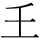
\includegraphics[width=3.8mm]{Chapter5/thengXkai.png}
 (09-17/09-01) provides evidence for the
change *k.l{\sil{ˤ}} \textgreater{} 見  \emph{k}- in type A syllables. Baxter \&
Sagart appear not to give examples of this sound change in type B
syllables.

\begin{description} \item
巠(
\includegraphics[width=3mm]{Chapter5/keng.png})  \emph{keng} \textless{} *k.l{\sil{ˤ}}- (09-01/0831a)
\item

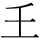
\includegraphics[width=3.8mm]{Chapter5/thengXkai.png}
(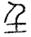
\includegraphics[width=4mm]{Chapter5/thengX.jpg})  
\emph{thengX} \textless{} *l̥- (09-17/0835a)
\item
梃  \emph{dengX} \textless{} *l{\sil{ˤ}}- (09-17/0835j)
\item
桯  \emph{yeng} \textless{} *l- (09-17/0835y)
\end{description}

§b. The series based on 丂 (13-03/13-43) provides evidence for the
change *k.r̥{\sil{ˤ}}- \textgreater{} 溪~ \emph{kh}- in type A syllables. Baxter
\& Sagart appear not to give examples of this sound change in type B
syllables.

\begin{description} \item
考  \emph{khawX} \textless{} *k.r̥{\sil{ˤ}}- (13-03d)
\item
老  \emph{lawX} \textless{} *r{\sil{ˤ}}- (13-43a)
\end{description}

§c. Baxter \& Sagart normally reconstruct a series that shows
 \emph{xiéshēng} contacts between velars and glottals as deriving from
inherited uvulars (cf. §). However, they also permit a pre-initial *k-
before {\sil{*ʔ-}} as an alternative explanation for such  \emph{xiéshēng}
series. They take the series based on 鬼(
\includegraphics[width=2mm]{Chapter5/kjwijX.png}) (28-01/28-09) as evidence
for the change {\sil{*k.ʔ-}} \textgreater{} 見  \emph{k}- (2014: 151).

\begin{description} \item
鬼(
\includegraphics[width=2mm]{Chapter5/kjwijX.png})  \emph{{\sil{kjwɨjX}}} \textless{} {\sil{*k.ʔ-}} (28-01/0569a)
 \item
畏(
\includegraphics[width=2.5mm]{Chapter5/'jwijH.png})  \emph{'{\sil{jwɨj}}H} \textless{} {\sil{*ʔ-}} (28-09/0573a)
\end{description}

Baxter \& Sagart make little effort to explain how they decide whether a
 \emph{xiéshēng} series should be analyzed as uvular initial versus
glottal initial with the occasional *k- prefix. It appears they prefer
not to have two  \emph{xiéshēng} series that write the same type of Old
Chinese syllable; by proposing {\sil{*k.ʔ-}} as the origin of 見  
\emph{k}- in the
reading of 鬼 \emph{{\sil{kjwɨjX}}} they are able to understand the series built
on 鬼 as encoding Old Chinese syllables of the shape *ʔuj as opposed to
the series built on 貴 as, which encodes Old Chinese syllables of the
shape *Quj \citep[151 n. 79 on p. 391]{Baxter2014OldChinese}. The inclusion
of readings with initial 曉 \emph{x}- and 以  \emph{y}- in the series
built on 貴 (31-02) essentially compels one to understand this series as
uvular initial in Baxter \& Sagart's system.\footnote{In violation of
  the \emph{xiéshēng} hypothesis, Baxter \& Sagart reconstruct many of
  the readings in the series built on 貴 (31-02) as having velar
  initials. e.g. 簣 \emph{khweajH} \textless{} *{\sil{kʰ}}{\sil{ˤ}}r- (31-02j), 聵
  \emph{ngweajH} \textless{} *[ŋ]{\sil{ˤ}}r- (31-02p). To my knowledge they
  have given no account of these reconstructions, but an obvious
  explanation to consider is that characters with velar readings are
  younger coinages, created after uvulars had already vanished.}

\begin{description} \item
靧  \emph{xwojH} \textless{} {\sil{*qʰ}}{\sil{ˤ}}- (31-02f)
\item
遺  \emph{ywij} \textless{} *{\sil{ɢ}}(r)- (31-02m)
\end{description}

§d. For *k- before resonants see §.

\paragraph{Tight pre-initials \textbf{*t-}}:
Tight pre-initial *t- explains the appearance of Middle Chinese
pronunciations with dental (\emph{shétóu} 舌頭  \emph{T}-),\footnote{Although
  Baxter \& Sagart include *t.q{\sil{ˤ}}- \textgreater{} 端  \emph{t}- in the
  table that summarizes the correspondences involving *t- (2014: 157), I
  am unable to locate an explicit discussion of this change in their
  volume.} palatal (\emph{zhāngzǔ} 章組  \emph{Tsy}-), or retroflex
initials (\emph{shéshǎng}舌上 \emph{Tr}-) in series that do not
predominantly contain readings with these initials 
\citep[157-159]{Baxter2014OldChinese}.

§a. The series based on 九(
\includegraphics[width=3mm]{Chapter5/kjuwX.png}) (04-12/13-23) provides evidence for the
change *t.kr- \textgreater{} 知 \emph{tr}-.

\begin{description} \item
肘(
\includegraphics[width=2mm]{Chapter5/trjuwX.png})  \emph{trjuwX} \textless{} *t.kr- (13-23a)
\item
九(
\includegraphics[width=3mm]{Chapter5/kjuwX.png})  \emph{kjuwX} \textless{} *k- (04-12a)
\end{description}

§b. The series based on 出 (31-16) provides evidence for the change
*t-{\sil{kʰ}}- \textgreater{} 昌 \emph{tsyh}- in type B syllables.

\begin{description} \item
出  \emph{tsyhwit} \textless{} *t.{\sil{kʰ}}- (31-16a)
\item
掘  \emph{gjut} \textless{} *g- (31-16s)
\end{description}

§c. The series based on 巠 (09-01) provides evidence for the change
*t.{\sil{kʰ}}r- \textgreater{} 徹 \emph{trh}- in type B syllables.

\begin{description} 
\item
徑  \emph{kengH} \textless{} *{\sil{kˤ}}- (09-01f)
\item
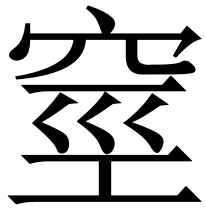
\includegraphics[width=3.4mm]{Chapter5/khengH.png}
 \emph{khengH} \textless{} *{\sil{kʰ}}{\sil{ˤ}}- (09-01j)
\item
陘  \emph{heng} \textless{} *g{\sil{ˤ}}- (09-01l)
\item
牼  \emph{kheang} \textless{} *{\sil{kʰ}}{\sil{ˤ}}r- (09-01q)
\item
䞓  \emph{trhjeng} \textless{} *t.{\sil{kʰ}}r- (09-01x)
\end{description}

§d. For *t- before resonants see §.

\paragraph{Tight stop pre-initials before
resonants}: Before resonants divergent dialect treatment of *p-, *t-,
and *k- on the way to Middle Chinese often leads to alternate readings
of the same character (Baxter \& Sagart 2014: 162).

\begin{description} \item
稟 (38-19a)  \emph{pimX} \textless{} *pr- \textless{} *p.r-, versus
 \emph{limX} \textless{} *p.r-
\item
慹 (37-08h)  \emph{tsyip} \textless{} *t- \textless{} *t.n-, versus
 \emph{nep} \textless{} *n{\sil{ˤ}}- \textless{} *t.n{\sil{ˤ}}-
\item
袂 (20-03d) \emph{kwe}t \textless{} *{\sil{kʷˤ}}- \textless{} *k.m{\sil{ˤ}}-, versus
 \emph{mjiejH} \textless{} *m- \textless{} *k.m-
\end{description}

\paragraph{Tight nasal pre-initials *m- and
*N-:} On the basis of  \emph{xiéshēng} evidence the tight
pre-initials *m- and *N- before obstruents are not easily distinguished
from each other nor are they distinguishable from simplex voiced
consonants. Nonetheless, *m-/*N- can be isolated on the basis of
 \emph{xiéshēng} evidence before the uvulars {\sil{*qʰ}}- and *{\sil{ɢ}}- (§a) and before
*r- (§b). In addition, *m- is identifiable on the basis of
 \emph{xiéshēng} evidence before (non-labial) nasals (§c).

§a. The pre-initials *m- and *N- before some uvulars are together
distinguishable from the voiced uvular *{\sil{ɢ}}- on the basis of
 \emph{xiéshēng} evidence. For example, the series built on 牙( )
(01-34/01-45) exhibits connections typical of a uvular series (見
 \emph{k}-, 影  \emph{'}-, 以 \emph{y}-), but it also contains readings
that begin with 疑  \emph{ng}-. One would like to find a way to credit
this 疑  \emph{ng}- also to an erstwhile uvular. Baxter \& Sagart's
explanation is a prefix *m- or *N- before a voiced uvular *{\sil{ɢ}} or the
voiceless aspirated uvular {\sil{*qʰ}}-, with the merger *m-{\sil{qʰ}}-, *m-ɢ-, *N-{\sil{qʰ}}-,
*N-ɢ- \textgreater{} 疑 \emph{ng}- (2014: 128-131). There is no way to
decide on the basis of  \emph{xiéshēng} evidence alone which of the four
uvular sources of 疑 \emph{ng}- is the correct re­con­struc­tion for a
given word.

\begin{description} \item
牙(
\includegraphics[width=2mm]{Chapter5/ngae.png} ) \emph{ngae} \textless{} *m.{\sil{qʰ}}r-, *m.ɢr-, *N.{\sil{qʰ}}r-, or *N.ɢr-
(01-34a)\footnote{\citet[131]{Baxter2014OldChinese} reconstruct this word
  with initial *m.{\sil{ɢˤ}}r-. It appears phonologically odd that *m.{\sil{qʰ}}-,
  *m.ɢ-, *N.{\sil{qʰ}}-, *N.{\sil{ɢ-}} develop to 疑  \emph{ng}-, but that *m.q- and
  *N.q- merge with *{\sil{ɢ}}-.}

\item
鴉  \emph{'ae} \textless{} q{\sil{ˤ}}r- (01-34h)

\item
舉(
\includegraphics[width=2.5mm]{Chapter5/kjoX.png}) \emph{kjoX} (01-45a)
\item
與(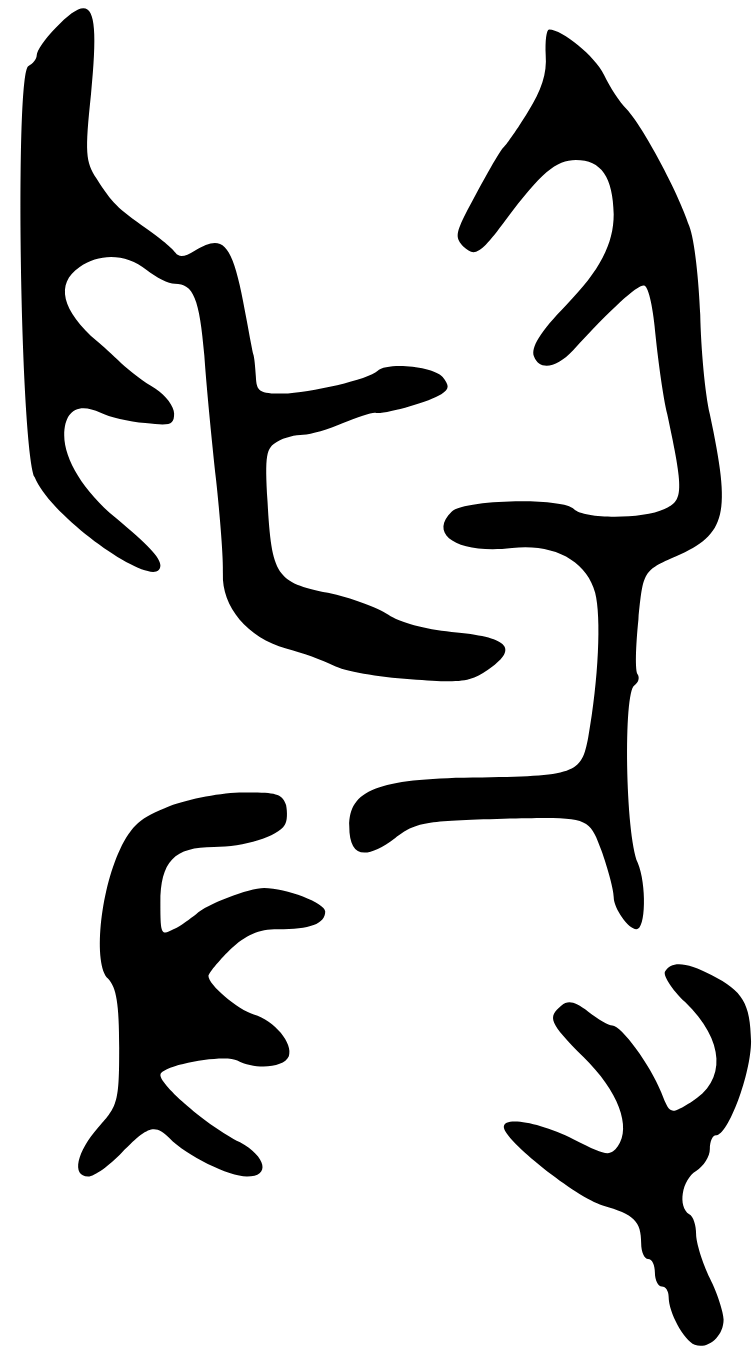
\includegraphics[width=2.5mm]{Chapter5/yoX.png}) \emph{yoX} \textless{} *{\sil{ɢˤ}}(r)- (01-45b)\footnote{Baxter \& Sagart
  (2014: 125) in fact reconstruct this word with initial *m-q(r)-
  relying on Mĭn evidence (cf. §a).}
\end{description}

§b. \citet[122, 133-134]{Baxter2014OldChinese}
%Baxter \& Sagart (2014: 122, 133-134) 
reconstruct *N.r- and *m.r-,
both merging with *l- (\textgreater{} 以  \emph{y}-), in order to account
for contacts between 以  \emph{y}- and 來  \emph{l}-. For example, the
character 斿 (13-33a) has the two readings  \emph{yuw} (\textless{} *l-
\textless{} *N.r- or *m.r-) and \emph{ljuw} (\textless{} *r-).\footnote{Baxter
  \& Sagart (2014: 134) postulate that Middle Chinese shows a mixture of
  two dialect developments. In one dialect *m.r- develops similarly to
  *l- (cf. 蠅  \emph{ying} \textless{} *m.r- {[}06-24a] and 黽
   \emph{meangX} \textless{} *m{\sil{ˤ}}r- {[}06-24d]). In the other dialect
  *m.r- merges with *m- (cf. 命  \emph{mjaengH} \textless{} *m.r-
  {[}09-32a] and 令  \emph{ljeng} \textless{} *r- {[}09-19a]). As
  reconstructing 命  \emph{mjaengH} with *mr- rather than *m.r- seems
  explanation enough, I am unable to follow their reasoning for the need
  to distinguish two dialect developments. One may further wonder what
  exact phonetic difference they suppose the notation *mr- versus *m.r-
  to reflect. }

§c. One context in which *m- makes its presence observable in
 \emph{xiéshēng} relationships is before the (non-labial) nasals *ŋ- and
*n-. Baxter \& Sagart reconstruct the Old Chinese clusters *m.ŋ- and
*m.n- (\textgreater{} 明 \emph{m}-) (2014: 132-133); these clusters
provide an ex­pla­na­tion for the occasional intrusion of 明
 \emph{m}-\emph{ }initial word into a series that predominantly has
initial 疑~ \emph{ng}- or 泥~ \emph{n}-. The series built on 兒 (07-11)
exhibits 明~ \emph{m}- in a 疑~ \emph{ng}- series.

\begin{description} \item
兒 \emph{nye} \textless{} *ŋ- (07-11a)
\item
倪 \emph{ngej} \textless{} *ŋ{\sil{ˤ}}- (07-11f)
\item
麑 \emph{mej} \textless{} *m.ŋ{\sil{ˤ}}- (07-11o)
\end{description}

The series built on 爾 (07-20) exhibits 明~ \emph{m}- in an 泥~ \emph{n}-
series.

\begin{description} \item
爾 \emph{nyeX} \textless{} *n- (07-20a)
\item
嬭 \emph{nejX} \textless{} *n{\sil{ˤ}}- (07-20d)
\item
彌 \emph{mjieX} \textless{} *m.n- (07-20m)
\end{description}

\paragraph{Tight pre-initials before uvulars
as a source of Middle Chinese velars :} 
\label{par:t-p-initials-before-ufvulars-as-a-source-of-MC-velars}
As discussed above, Baxter \&
Sagart reconstruct series that mix glottals and velars as uvulars (§),
but the discussion so far has not treated the velar stops appearing in
such series. Baxter \& Sagart propose that tightly attached stop
pre-initials are the origin of velar initial readings appearing in
uvular series (\citet[28, 45, 168-170]{Baxter2014OldChinese})\footnote{Sagart
  \& Baxter (2009: 231) proposed that `loose' pre-initials conditioned
  the shift from uvulars to Middle Chinese velars, but because some of
  the relevant words do not have `softened' initials in proto-Mǐn they
  have revised their proposal to instead suggest `tight' pre-initials
  before uvulars are the source of the relevant cases of velars (Baxter
  \& Sagart 2014: 385 note 24). For tight pre-initial *N- and *s- before
  uvulars see respectively §a and §e-g.}

§a. The series built on 公 (12-13) provides evidence of *C.q{\sil{ˤ}}- and the
change *C.q{\sil{ˤ}}- \textgreater{} 見~ \emph{k}- in type A syllables.

\begin{description} \item
公(
\includegraphics[width=3mm]{Chapter5/kuwng.png}) \emph{kuwng} \textless{} *C.q{\sil{ˤ}}- (12-13/1173a)
\item
瓮 `\emph{uwngH} \textless{} {\sil{*qˤ}}- (12-13g)
\item
容(
\includegraphics[width=4mm]{Chapter5/yowng.png}) \emph{yowng} \textless{} *{\sil{ɢ}}r- (12-11a)
\end{description}

§b. The series built on 京 (03-10) provides evidence of *C.qr- and the
change *C.qr- \textgreater{} 見~ \emph{k}- in type B syllables.

\begin{description} \item
景 \emph{kjaengX} \textless{} *C.qr- (03-10/0755d)
\item
影 \emph{'jaengX} \textless{} *qr- (03-21/0756a)
\end{description}

§c. The series built on 衍 (24-29) provides evidence of *C.{\sil{qʰ}}r- and the
change of *C.{\sil{qʰ}}r- \textgreater{} 溪~ \emph{kh}- in type B syllables.

\begin{description} \item
衍  \emph{yenH} \textless{} *N-q(r)- (24-29/24-29a)\footnote{Baxter \&
  Sagart reconstruct *N-q(r)- rather than *{\sil{ɢ}}- on the presumption that 愆
  *C.{\sil{qʰ}}ra[n] \textgreater{}  \emph{khjen} `exceed, err' and 衍
  *N-q(r)anʔ \textgreater{}  \emph{yenX} `overflow' derive from the same
  root (2014: 169).}

\item
愆 \emph{khjen} \textless{} *C.{\sil{qʰ}}r- (24-29/24-29b)
\end{description}

§d. The series built on 气 (30-01) provides evidence of *C.{\sil{qʰ}}- and the
change *C.{\sil{qʰ}}- \textgreater{} 溪~ \emph{kh}- in type B syllables.

\begin{description} \item
乞 \emph{{\sil{khjɨ}}t} \textless{} *C.{\sil{qʰ}}- (30-01/0517f)
\item
氣 \emph{{\sil{xjɨj}}H} \textless{} {\sil{*qʰ}} (30-01/0517c)
\end{description}

§e. The series built on 吅 provides evidence of *C.{\sil{qʷʰ}}- and the change
*C.{\sil{qʷʰ}}- \textgreater{} 溪~ \emph{kh}- 
\citep[170]{Baxter2014OldChinese}.

\begin{description} \item
吅 \emph{xjwon} \textless{} {\sil{*qʷʰ}}- (25-02/0158-)
\item
勸 \emph{khjwonH} \textless{} *C.{\sil{qʷʰ}}- (25-02/0158s)
\end{description}

§f. A sequence of *m- or *N- and a uvular give rise to initial
疑~ \emph{ng}- (cf. §a).

\subsection{Reconstructing tight pre-initials on the basis of
morphological
speculation}

\paragraph{} 
\label{par:recon-t-p-initials-on-morphological-speculation}
Baxter \& Sagart reconstruct seven morphological affixes: the
prefixes *s-, *N-, *m-, *t-, and *k-, an infix *-r-, and a suffix *-s
(2014: 53-59, cf. §§-). They distinguish between a verb valence
increasing *s- prefix and a circumstantial noun *s- prefix (2014: 56).
Their prefix *N- decreases verb valence (2014: 54, cf. §§-).\footnote{Both
  Ancient Egyptian and the Semitic languages also evince an *s- valence
  increasing and *N- valence decreasing prefix (Moscati 1964: 125-127).
  This is a remarkable morphological coincidence between Old Chinese, as
  Baxter \& Sagart reconstruct it, and Afro-Asiatic. } They distinguish
five different *m- prefixes (2014: 54-56, cf. § and §). The presumed *t-
prefix they do not use to explain relationships between words, but
simply note its occurrence in some words (2014: 56-57); they never
reconstruct the pre-initial *t- on the basis of morphological
speculation.\footnote{The pair 臭  \emph{tsyhuwH} \textless{} *t-{\sil{qʰ}}u(ʔ)-s
  (13-12a) `foul smell ` and 朽  \emph{xjuwX} \textless{} {\sil{*qʰ}}(r)uʔ
  (13-03m) `rot, decay' is perhaps the one case in which they presume a
  pre-initial *t- on the basis of etymological speculation (Baxter \&
  Sagart 2014: 57). However, they do not discuss the pair explicitly, so
  one cannot be sure on what grounds they reconstruct initial 昌
   \emph{tsyh}- as *t-{\sil{qʰ}} in the first word. For example, one might regard
  the series built on 臭 (13-12) as uvular because of the velar
  fricative initial of 嗅 \emph{xjuwH} (13-12c), cf. §§-. } The presumed
prefix *k- nominalizes verbs (2014: 57, cf. §). The infix *-r- and final
*-s are reconstructed using the conventional sources for Old Chinese
historical phonology; Baxter \& Sagart assign them with a morphological
meaning, but, unlike for the prefixes, do not employ morphological
argumentation to posit their existence.

\paragraph{The tight pre-initial
*s-:} All researchers appears to concur that *s- had a
causative function in Old Chinese (cf. Handel 2012). The credit for this
proposal, as well as a proposed link between *s- in Chinese and the
Tibetan causative prefix \emph{s}-, typically goes to Conrady (1896).
However, Conrady did not propose Chinese *s- in the circumstances in
which Karlgren, Li, Baxter, and Sagart do, but rather in those places
where Baxter \& Sagart would reconstruction voiceless nasals (see
Conrady 1896: 156).

Baxter \& Sagart propose two different morphological functions for an
*s- prefix, a valency increasing verb prefix and a prefix that ``derives
circumstantial nouns (place, time, instrument)'' (2014: 56). Outside of
the initial presentation of the two prefixes, in their discussion of
words presumed to have an etymological relationship Baxter \& Sagart
generally fail to make explicit which of the two *s- prefixes they
believe is at play. They employ etymological arguments in favor of *s-
prefix origins of Middle Chinese 心~ \emph{s}- (cf. §), 生~ \emph{sr}-
(cf. §), 邪~ \emph{z}- (cf. §), 精~ \emph{ts}-, 莊~ \emph{tsr}- (cf. §),
清~ \emph{tsh}- (cf. §), and 初~ \emph{tsrh}- (cf. §).

§a. They provide the following four pairs of words to exemplify the
valency increasing prefix.

\begin{description} \item
烝 \emph{tsying} \textless{} *təŋ (06-10h) `rise (of steam)'; 升
 \emph{sying} \textless{} *s-təŋ (06-16a) `lift up, to save, to present
to'
\item
諤 \emph{ngak} \textless{} *ŋ{\sil{ˤ}}ak (02-14k) `speak frankly'; 愬 \emph{suH}
\textless{} *s-ŋ{\sil{ˤ}}ak-s (02-34b) `complain, accuse'
\item
當 \emph{tang} \textless{} *t{\sil{ˤ}}aŋ (03-32q) `match (v.); have the value
of, rank with'; 商 \emph{syang} \textless{} *s-taŋ (03-40a) `estimate'
\item
視 \emph{dzyijX} \textless{} *gijʔ (26-07h) `look, see'; 示 \emph{zyijH}
\textless{} *s-gijʔ-s (26-07a) `show (v.)'
\end{description}

§b. They provide the following three pairs of words to exemplify the
circumstantial noun prefix.\footnote{Baxter \& Sagart also give an
  example of the circumstantial noun prefix, in which the prefix is
  loose, viz. 以  \emph{yiX} \textless{} *ləʔ `take, use', 鈶 \emph{ziX}
  \textless{} *sə.ləʔ `handle of plow or sickle ` (i.e. `instrument of
  holding') (2014: 56).}

\begin{description} \item
屰 \emph{ngjaek} \textless{} *ŋrak (02-14a) `go against, reverse'; 朔
 \emph{sraewk} \textless{} *s-ŋrak (02-34a) `first day of month' (when
the moon changes from waning to waxing) (cf. p. n. )
\item
通 \emph{thuwng} \textless{} *l̥{\sil{ˤ}}oŋ (12-10r) `penetrate'; 窗
 \emph{tsrhaewng} \textless{} *s-l̥{\sil{ˤ}}roŋ (12-19-) `window' (i.e. `where
light penetrates')
\item
亡 \emph{mjang} \textless{} *maŋ (03-65a) `flee; disappear; die'; 喪
 \emph{sang} \textless{} *s-m{\sil{ˤ}}aŋ (03-54a) `mourning, burial' (i.e.
'circumstances associated with death')
\end{description}

The second and third example of the circumstantial noun prefix are not
flawless. The derivation of 窗  \emph{tsrhaewng} \textless{} *s-l̥{\sil{ˤ}}roŋ
`window' from 通  \emph{thuwng} \textless{} *l̥{\sil{ˤ}}oŋ `penetrate' involves an
-r- infix in addition to the *s- prefix and the derivation from of 喪
 \emph{sang} \textless{} *s-m{\sil{ˤ}}aŋ `mourning, burial' from 亡~ \emph{mjang}
\textless{} *maŋ `flee; disappear; die' includes an unexplained change
from a type B syllable to a type A syllable.

\paragraph{Tight pre-initial *s- as an origin
of Middle Chinese 心~} \emph{\textbf{s}}\textbf{-}\textbf{:} On
the basis of etymological argumentation Baxter \& Sagart reconstruct
both *s.ts- (cf. §a) and *s.ts{\sil{ʰ}}{\sil{ˤ}}- (§b) as origins for 心~ \emph{s}-.

§a. Baxter \& Sagart offer two pair of etymologically related words in
support of a change *s.ts- \textgreater{} 心~ \emph{s}- 
\citeyearpar[136]{Baxter2014OldChinese}.

\begin{description} \item
節 \emph{tset} \textless{} *ts{\sil{ˤ}}ik (29-30e) `joint of bamboo'; 膝
 \emph{sit} \textless{} *s.tsik (29-32c) `knee'
 \item
㕚 , 爪  \emph{tsraewX} \textless{} *[ts]{\sil{ˤ}}ruʔ (13-60a, 13-59a)
`claw'; 搔  \emph{saw} \textless{} *s-{[}ts]{\sil{ˤ}}u (13-60f) `scratch (v.)'
\end{description}

These proposals are not without difficulties. The derivation of `knee'
from `joint of bamboo' is neither an instance of the valence increasing
prefix nor of the circumstantial noun prefix. Sagart \& Baxter instead
suggest that perhaps ``we have a Chinese instance of the
T{[}ibeto-]B{[}urman] *s- animal (and body-part?) prefix from TB
*sya -- `flesh''' (2012: 45), which Benedict (1972: 106) has proposed. I
concur with Chang that Benedict's animal prefix is ``a dubious
proposition'' (1973: 336).\footnote{The fact that `joint of bamboo' is
  type A whereas `knee' is type B further complicates the relationship
  between the two words. There are other examples of alternations
  between type A and type B words (Baxter \& Sagart 1997: 61-62), with
  the pair 內 \emph{nop} \textless{} *n{\sil{ˤ}}{[}u]p `bring or send in'
  (37-16e) and 入 \emph{nyip} \textless{} *n{[}u]p `enter' (37-16a) as
  a well known case. No explanation has been put forward for the origin
  or derivational meaning of such patterns.} The proposal to derive
'scratch' from `claw' with a denominative *s- is less problematic, but
the absence of medial -r- in the verb `scratch' is an obstacle to this
proposal.

§b. Baxter \& Sagart offer one pair of etymologically related words in
support of a change *s.ts{\sil{ʰ}}{\sil{ˤ}}- \textgreater{} 心~ \emph{s}- 
\citeyearpar[139]{Baxter2014OldChinese}.

\begin{description} \item
清 \emph{tshjeng} \textless{} *ts{\sil{ʰ}}eŋ `clear (adj.)'; 星  \emph{seng}
\textless{} *s-ts{\sil{ʰ}}{\sil{ˤ}}eŋ `star' (i.e. that which is bright)
\end{description}

They acknowledge the difficulty that `clear' is type B whereas `star' is
type A. This proposed pair of cognates would not be compelling except
that words for `star' in the Mǐn dialects support initial *tsh- (cf.
Amoy /ts{\sil{ʰ}}ĩ 1/, §).

\paragraph{Tight pre-initial *s- as an origin of Middle Chinese
生 \emph{sr-}:} On the basis of the following pair of
words, Baxter \& Sagart reconstruct *s-{\sil{qʰ}}r- as one source of Middle
Chinese 生  \emph{sr}- 
\citeyearpar[129]{Baxter2014OldChinese}.

\begin{description}
\item
許 \emph{xjoX} \textless{} {\sil{*qʰ}}(r)aʔ (01-30i) `place (n.)'; 所
 \emph{srjoX} \textless{} *s-{\sil{qʰ}}raʔ (01-63a) `place (n.); that which'
\end{description}

Without further discussion this derivation is unconvincing. Note however
that the line 伐木許許 "chop trees `hack-hack'" of Ode 165.2 is quoted
in the entry for the character 所 in the 說文解字  \emph{Shuōwén Jiězì}
as 伐木所所; thus, the pronunciations of 許 (01-30i) and 所 (01-63a)
must have had very similar pronunciations, or at least both reflected
pronunciations that were suitable as onomatopoeia for the sound of
chopping wood.\footnote{I thank Adam Smith for drawing my attention to
  this use of 許 (01-30i) and 所 (01-63a) (\emph{per litteras} 25 May
  2017).}

\paragraph{Tight pre-initial *s- as an origin
of Middle Chinese 邪 \emph{\textbf{z}}\textbf{-:}} 
\label{par:tight-pre-initial-s-for-MC-z-2}
\citet[141-142]{Baxter2014OldChinese}
propose that pre-initial *s- before voiced obstruents in
type B syllables is one source of Middle Chinese 邪 \emph{z}-. They
propose *s.ɢ- \textgreater{} 邪  \emph{z}- on the basis of
 \emph{xiéshēng} evidence (cf. §a). They also propose *s.d-
\textgreater{} 邪  \emph{z}- on the basis of proto-Mǐn and loanwords into
non-Sinitic languages (cf. §). For the parallel, but yet more
complicated *s-m-t- \textgreater{} 邪  \emph{z}- they return to
etymological argumentation.

\begin{description} \item
著 \emph{trjak} \textless{} *trak (01-38n') `place (v.)'; 席  \emph{zjek}
\textless{} *s-m-tAk (02-29a) `mat' (i.e. `place for putting things')
\end{description}

Baxter \& Sagart do not however account for the morphological function
of the *m- prefix in `mat' nor the -r- infix in `place (v.)'.

\paragraph{Tight pre-initial *s- as an origin of Middle Chinese
\textbf{船}  \emph{\textbf{zy}}-: }In favor of the change *s.g-
\textgreater{} \textbf{船}  \emph{zy}- 
\citet[56]{Baxter2014OldChinese} point the the following verb pair.

\begin{description} \item
視 \emph{dzyijX} \textless{} *gijʔ (26-07h) `look, see'; 示  \emph{zyijH}
\textless{} *s-gijʔ-s (26-07a) `show (v.)'\footnote{Handel (2012: 76)
  points out that this pair is the only example of a causative *s-
  prefix before non-resonant velar initials in Baxter \& Sagart's
  system.}
\end{description}

\paragraph{Tight pre-initial *s- as an origin
of Middle Chinese \textbf{精~} \emph{ts}- and
莊~ \emph{tsr}-:}
Baxter \& Sagart (2014:
136) propose a change *s.t{\sil{ˤ}}- \textgreater{} 精~ \emph{ts}- on the basis
of presumed etymological relationships between words with Middle Chinese
initial 端 \emph{t}- and those with initial 精~ \emph{ts}-.

\begin{description} \item
登 \emph{tong} \textless{} *t{\sil{ˤ}}əŋ (06-09e) `ascend'; 增 \emph{tsong}
\textless{} *ts{\sil{ˤ}}əŋ \textless{} *s-t{\sil{ˤ}}əŋ (06-19c) `increase (v.)'
\end{description}

Baxter \& Sagart (2014: 136) similarly propose a change *s-t{\sil{ˤ}}r-
\textgreater{} 莊~ \emph{tsr}- on the basis of presumed etymological
relationships between words with Middle Chinese initial 知  \emph{tr}-
and those with initial 莊~ \emph{tsr}-.

\begin{description} \item
謫 \emph{treak} \textless{} *t{\sil{ˤ}}rek (07-12r) `blame (v.)';\footnote{Baxter
  \& Sagart in fact reconstruct 謫 \emph{treak} \textless{} *C.t{\sil{ˤ}}rek
  (07-12r) `blame (v.)', positing the *C. pre-initial on the basis of
  Vietnamese  \emph{dức} {[}zɯk D1] `reprove' (2014: 136). } 責
 \emph{tsreak} \textless{} *ts{\sil{ˤ}}rek \textless{} *s-t{\sil{ˤ}}rek (08-14m) `demand
payment'
\end{description}

The derivation from `blame' to `demand payment' is not obviously a case
of valence increase.

\paragraph{Tight pre-initial *s- as an origin
of Middle Chinese 清\textbf{~} \emph{\textbf{tsh}}\textbf{-:
}}Baxter \& Sagart propose the change *s.r̥{\sil{ˤ}}- \textgreater{}
清~ \emph{tsh}- to account for Middle Chinese doublets in which one word
begins with 清~ \emph{tsh}- and the other with 生~ \emph{sr}-; they credit
these doublets to divergent dialect developments (2014: 150).

\begin{description} \item
採 \emph{tshojX} \textless{} *s.r̥{\sil{ˤ}}əʔ (04-44d) `pluck, reap'; 嗇
 \emph{srik} \textless{} *s.rək (04-44d) `reap'
 \item
彩 \emph{tshojX} \textless{} *s.r̥{\sil{ˤ}}əʔ (04-44a) `colorful'; 色  \emph{srik}
\textless{} *s.rək (05-31a) `color; countenance'
\end{description}

\paragraph{Tight pre-initial *s- as
an origin of Middle Chinese
初~ \emph{tsrh}-:} Baxter \& Sagart
propose a change *s-t{\sil{ʰ}}{\sil{ˤ}}- \textgreater{} 初~ \emph{tsrh}- on the basis of
the following verb pair, in which they see the valence increasing *s-
prefix at play.

\begin{description} \item
推 \emph{thwoj} \textless{} *t{\sil{ʰ}}{\sil{ˤ}}uj (28-11a') `push away'; 催
 \emph{tshwoj} \textless{} *s-t{\sil{ʰ}}{\sil{ˤ}}uj (28-11j') `urge, repress'
\end{description}

\paragraph{The tight nasal p}re-initial *m-
and\textbf{*N-:} The nasal prefixes *m- and *N- of Baxter \& Sagart's
system are almost always impossible to distinguish using  \emph{xiéshēng}
evidence; in addition, before stops using  \emph{xiéshēng} evidence they
are indistinguishable from plain voiced onsets. Nonetheless, presumed
morphology, as well as proto-Mǐn (cf. §) and loanwords into Vietnamese
(cf. §), allow these two pre-initials to be differentiated from each
other and from voiced stops in many circumstances.

\paragraph{Pre-initial *N-}: To explains
morphological alternations between transitive and intransitive verbs
Pulleyblank (1973: 114) proposed a prefix (that he reconstructed *ɦ)
which voices a voiceless initial while making a verb intransitive. Often
both the transitive and the intransitive verb are written with the same
character.

\begin{description} \item
見 (23-02a) \emph{kenH} `see',  \emph{henH} `appear'
 \item
敗 (21-35f) \emph{paejH} `defeat',  \emph{baejH} `suffer defeat'
\item
壞 (28-06d) \emph{kweajH} `destroy, ruin',  \emph{hweajH} `be destroyed'
\item
斷 (25-22a) \emph{twanX} `cut in two',  \emph{dwanX} `be cut in two'
\item
折 (21-19a) \emph{tsyet} `break, bend' (v.t.),  \emph{dzyet} `bend'
(v.i.)
\end{description}

Sagart (1993: 244) proposed that the Chinese intransitive voicing prefix
must be some kind of nasal on the basis of the Mien high tone voiced
initial in the Chinese loanword 折 dzɛ́ʔ `be cracked', which suggests a
proto-Yao pre-nasalized voiceless initial. Baxter \& Sagart have changed
little in their evidence for and explanation of *N- since 1997 (cf.
Baxter \& Sagart 1997: 45-47). In their recent book they present the
following verb pairs as evidence of *N- (2014: 116-123).

\begin{description} \item
見  \emph{kenH }\textless{} *[k]{\sil{ˤ}}en-s (23-02a) `see'; 見 \emph{henH}
\textless{} *N-{[}k]{\sil{ˤ}}en-s (23-02a) `appear'
\item
敗  \emph{paejH} \textless{} *p{\sil{ˤ}}ra{[}t]-s (21-35f) `defeat'; 敗
 \emph{baejH} \textless{} *N-p{\sil{ˤ}}ra{[}t]-s (21-35f) `suffer defeat'
\item
壞  \emph{kweajH} \textless{} *[k]{\sil{ˤ}}ruj-s (28-06d) `destroy, ruin'; 壞
 \emph{hweajH} \textless{} *N-{[}k]{\sil{ˤ}}ruj-s (28-06d) `be destroyed'
\item
斷  \emph{twanX} \textless{} *t{\sil{ˤ}}o[n]ʔ (25-22a) `cut in two'; 斷
 \emph{dwanX} \textless{} *N-t{\sil{ˤ}}o[n]ʔ (25-22a) `be cut in two'
\item
折  \emph{tsyet} \textless{} *tet (21-19a) `break, bend' (v.t.); 折
 \emph{dzyet} \textless{} *N-tet (21-19a) `bend' (v.i.)
\item
夾  \emph{keap} \textless{} *C.{\sil{kˤ}}rep (35-03a) `press between'; 狹
 \emph{heap} \textless{} *N-{\sil{kˤ}}rep (35-03e) `narrow'
\item
置  \emph{triH} \textless{} *trək-s (05-12g) `put, place; set upright';
直 \emph{drik} \textless{} *N-trək (05-12a) `straight'
\item
清  \emph{tshjeng} \textless{} *ts{\sil{ʰ}}eŋ (09-25i') `clear (adj.)'; 晴
 \emph{dzjeng} \textless{} *N-ts{\sil{ʰ}}eŋ (09-25-) `clear (of weather)'
\end{description}

§a. To explain apparent etymological connections between words with
Middle Chinese initial 以  \emph{y}- or  \emph{d}- (normally from OChi.
*l-) and Middle Chinese initial \emph{l}- (from OChi. *r-), Baxter \&
Sagart (2014: 122) posit an original *N-r- that merges with *l- (i.e.
OChi. *N-r- \textgreater{} *l- \textgreater{} MChi. 以  \emph{y}- and
OChi. *N-r{\sil{ˤ}}- \textgreater{} *l{\sil{ˤ}}- \textgreater{} MChi.  \emph{d}-).

\begin{description} \item
流  \emph{ljuw} \textless{} *ru (13-46a) `flow (v.)'; 游 \emph{yuw}
\textless{} *lu \textless{} *[N-]ru (13-33f) `float, swim'
\item
旒  \emph{ljuw} \textless{} *[r]u (13-46c) `pendants of a banner or
cap'; 斿 \emph{yuw} \textless{} *lu \textless{} *[N.]ru (13-33a)
`pendants of a banner'
\item
儽  \emph{lwojH} \textless{} *[r]{\sil{ˤ}}uj-s (28-15p) `exhausted'; 隤
 \emph{dwoj }\textless{} *l{\sil{ˤ}}wəj \textless{} *N-r{\sil{ˤ}}uj (28-13a) `exhausted'
\item
婪  \emph{lom} \textless{} *[r]{\sil{ˤ}}{[}ə]m (38-18i) `covet'; 淫
 \emph{yim} \textless{} *ləm \textless{} *N.r{[}ə]m (38-15b) `excess;
licentious'
\end{description}

Baxter \& Sagart find no reason to reconstruct *N- before voiceless
resonants (2014: 122).

§b. Before uvulars the prefix *N- induces a velar nasal initial (Baxter
\& Sagart 2014: 121).

\begin{description} \item
嚇  \emph{xaek} \textless{} {\sil{*qʰ}}{\sil{ˤ}}rak (02-10b) `to frighten'; 愕
\emph{ngak} \textless{} *N-{\sil{qʰ}}{\sil{ˤ}}ak (02-14h) `scared'
\item
夏  \emph{haeX} \textless{} *{\sil{[ɢ]ˤ}}raʔ (01-15a) `great'; 雅
 \emph{ngaeX} \textless{} *N-{\sil{ɢˤ}}raʔ (01-34g) `proper, refined'
\end{description}

The hypotheses *N-{\sil{qʰ}} \textgreater{} \emph{ng-} and *N-ɢ \textgreater{}
 \emph{ng}- also receive support from  \emph{xiéshēng} evidence (§a).

\paragraph{Pre-initial *m-:} Baxter \& Sagart
propose a number of morphological *m- prefixes in Old Chinese, including
a volitional verb prefix, a `human body part prefix', and an `animal
prefix' (2014: 54-56). The verbal prefix *m-, was the first *m- prefix
to emerge in their work, and it emerged as distinct from *N- only slowly
in their system. Some of Baxter's 1992 examples of *N- pair a noun with
a voluntary verb, rather than a transitive with an intransitive verb
(Baxter 1992: 218-219). Such cases instil the suspicion that there is a
morpheme other than the detransitivizing *N- at play.

\begin{description} \item
朝 (16-17a) \emph{trjew} `morning',  \emph{drjew} `(morning ceremony:)
audience, court, go to the court of'

\item
背 (05-32e) \emph{pwojH} `the back',  \emph{bwojH} `turn the back'
\end{description}

Sagart (1999a: 79-86) proposes a prefix *m- with volitional meaning. He
presents three examples with lateral initial verbs.

\begin{description} \item
順  \emph{zywinH} \textless{} *m-lun-s in 1999, now *Cә.lu[n]-s
(34-20c) `follow; obey' (cf. 循  \emph{zwin} \textless{} *sə.lu[n]
{[}34-21f] `follow')

\item
贖  \emph{zyowk} \textless{} *m-l{[}u]k in 1999, now *Cə.lok (14-14t)
'redeem' (cf. 賣 \emph{yuwk} \textless{} *luk {[}14-14a] `sell')

\item
射  \emph{zyek} \textless{} *m-lak in 1999, now *Cә.lAk (02-26a) `hit
with bow and arrow' (cf. 釋  \emph{syek} \textless{} *l̥Ak {[}02-25l]
'release; dissolve')
\end{description}

Baxter \& Sagart no longer reconstruct these three words with a *m-
pre-initial; whether or not they would still regard the comparisons made
(e.g. of 順 \emph{zywinH} `follow; obey' to 循  \emph{zwin} `follow') as
reflecting genuine etymological relationships is unclear.\footnote{It is
  worrying that the semantic affect of *m- has remained stable since
  1999 although the words that originally motivated these semantics are
  no longer taken as examples of this prefix. This paradox suggests that
  `volition' may be too broad a meaning, and allow for any number of
  potentially invalid etymological proposals.}

Nonetheless, Baxter \& Sagart have subsequently found quite a few of
potential examples of this *m- voluntary prefix. Although in Middle
Chinese (and Sinitic loans in Hmong-Mien) *N- and *m- are
indistinguishable, in proto-Mĭn and Sinitic loans into Vietic the two
prefixes can be distinguished (§ and §).\footnote{With regard to Chinese
  external evidence Sagart \& Baxter (2010) point to an \emph{m}- prefix
  in Daai Chin, as described by Hartmann 2001. Although `volition' does
  appear to cover well the examples that Hartmann presents, this is not
  her analysis of the prefix's function. Also compare So-Hartmann (2009:
  55-56).}

§a. Baxter \& Sagart propose an *m- prefix before voiceless stops on the
basis of apparent etymological relationships between Middle Chinese
words with voiced initials and those with voiceless initials (2014:
123).

\begin{description} \item
包 \emph{paew} \textless{} *p{\sil{ˤ}}ru (13-72a) `wrap, bundle'; 抱  \emph{bawX}
\textless{} *[m-p]{\sil{ˤ}}uʔ (13-72j) `carry in the arms' (volitional)

\item
拄 \emph{trjuX} \textless{} *troʔ (10-19e) `prop up, support (v.)'; 樹
 \emph{dzyuX} \textless{} *m-toʔ (10-22j) `plant (v.); place upright'
(volitional)

\item
合 \emph{kop} \textless{} *{\sil{kˤ}}op (37-01a) `together; put together;
combined'; 合 \emph{hop} \textless{} *m-{\sil{kˤ}}op (37-01a) `come together;
bring together' (volitional)

\item
誡  \emph{keajH} \textless{} *{\sil{kˤ}}rək-s (04-03c) `warn'; 忌 \emph{giH}
\textless{} *m-k(r)ək-s (04-05s) `warn; avoid' (volitional)

\item
肚  \emph{tuX} \textless{} *t{\sil{ˤ}}aʔ (01-36-) `belly, stomach'; 肚 \emph{duX}
\textless{} *m-t{\sil{ˤ}}aʔ (01-36-) `belly'

\item
兜  \emph{tuw} \textless{} *t{\sil{ˤ}}o (10-12a) `helmet, hood'; 頭 \emph{duw}
\textless{} *[m-t]{\sil{ˤ}}o (10-16e) `head (body part)'

\item
髀  \emph{pjieX} \textless{} *peʔ (07-29f) `femur, haunch'; 髀
 \emph{bejX} \textless{} *m-p{\sil{ˤ}}eʔ (07-29f) `femur'
\end{description}

§b. They propose an *m- prefix before aspirated voiceless stops on the
basis of apparent etymological relationships between Middle Chinese
words with voiced initials and those with aspirated initials (Baxter \&
Sagart 2014: 128).

\begin{description} \item
奉  \emph{phjowngX} \textless{} *p{\sil{ʰ}}(r)oŋʔ (12-25z) `hold with both hands;
to present; receive'; 奉 \emph{bjowngX} \textless{} *m-p{\sil{ʰ}}(r)oŋʔ (12-25z)
`present (v.) with both hands'
\item
撤  \emph{trhjet} \textless{} *t{\sil{ʰ}}ret (21-20b) `remove, take away'; 撤
 \emph{drjet} \textless{} *m-t{\sil{ʰ}}ret (21-20b) `remove, take away'
\item
土  \emph{thuX} \textless{} *t{\sil{ʰ}}{\sil{ˤ}}aʔ (01-36a) `earth'; 社  \emph{dzyaeX}
\textless{} *m-t{\sil{ʰ}}Aʔ (01-36j) `sacrifice to the spirit of the soil'
\item
倉  \emph{tshang} \textless{} *ts{\sil{ʰ}}{\sil{ˤ}}aŋ (03-48a) `granary'; 藏  \emph{dzang}
\textless{} *m-ts{\sil{ʰ}}{\sil{ˤ}}aŋ (03-49g') `store (v.)'
\end{description}

\begin{description} \item
牼  \emph{kheang} \textless{} *{\sil{kʰ}}{\sil{ˤ}}reŋ (09-01q) `shank bone'; 脛
 \emph{hengH} \textless{} *m-{\sil{kʰ}}{\sil{ˤ}}eŋ-s (09-01k) `leg, shank'
\end{description}

§c. The voicing effect of the prefix naturally is unrecognizable when it
acts upon voiced roots. In these cases, it is alone the semantic
difference between different functions of the same Middle Chinese
reading (or eadings that coincidentally differ only by tone) that leads
to Baxter \& Sagart postulating the *m- prefix (2014: 131).

\begin{description} \item
平  \emph{bjaeng} \textless{} *breŋ (09-26a) `even (adj.)'; 平
 \emph{bjaeng} \textless{} *m-breŋ (09-26a) `make even'
\item
下  \emph{haeX} \textless{} *g{\sil{ˤ}}raʔ (01-14a) `down'; 下 \emph{haeH}
\textless{} *m-g{\sil{ˤ}}raʔ-s (01-14a) `descend'
\item
毒  \emph{dowk} \textless{} *[d]{\sil{ˤ}}uk (14-05a) `poison (n.)'; 毒
*dawH\footnote{The Middle Chinese reading is unattested (Baxter \&
  Sagart 2014: 132 note 55 on p. 389)} \textless{} *m-{[}d]{\sil{ˤ}}uk-s
(14-05a) `to poison (v.)' (volitional)
\end{description}

§d. In principle, Baxter \& Sagart reconstruct *m.l- when a Middle
Chinese word with initial 船 \emph{zy}- has etymological connections
with lateral initials (2014: 133), but they put forward only one
somewhat problematic example.

\begin{description} \item
塍  \emph{zying} \textless{} *m.ləŋ (06-09n) `raised path between
fields'; 勝 \emph{syingH} \textless{} *l̥əŋ-s (06-09p) `overcome;
surpass'
\end{description}

The example is problematic because the *m- does not have an obvious
function and because the difference between the voiced lateral in 塍
 \emph{zying} \textless{} *m.ləŋ (06-09n) `raised path between fields'
and the voiceless lateral in 勝 \emph{syingH} \textless{} *l̥əŋ-s
(06-09p) `overcome; surpass' is left unaccounted for.

§e. The `animal prefix' is ground enough for Baxter \& Sagart to
reconstruct *m- before uvulars in words for `frog' and `bird', where
variant pronunciations show voicing alternation (2014: 55).

鼃  \emph{'wea, `wae} \textless{} {\sil{*qʷˤ}}re `frog'; 鼃  \emph{hwea, hwae}
\textless{} *m-q{\sil{ʷˤ}}re `frog'

鷽  \emph{aewk} \textless{} {\sil{*qˤ}}ruk (14-03h) (`a kind of bird'); 鷽
 \emph{haewk} \textless{} *m-q{\sil{ˤ}}ruk (`a kind of bird')

§f. Baxter \& Sagart (2014: 55) also see the `animal prefix' in words
for `fawn' and `deer'. In the case of `fawn'  \emph{xiéshēng} evidence
supports the reconstruction (cf. §c) and for `deer' the form of the word
in Bùyāng dialect confirms the pre-initial.

\begin{description} \item
麑  \emph{mej} \textless{} *m-ŋ{\sil{ˤ}}e (07-11o) `fawn'
\end{description}

鹿  \emph{luwk} \textless{} *mə-r{\sil{ˤ}}ok `deer' (cf. Bùyāng 布央 /ma 0 lok 8/
`deer')

\paragraph{Pre-initial *k-:} Baxter \& Sagart
propose a pre-initial *k- in three words on the basis of the
etymological speculation that they are nouns that derive from verbs
(2014: 152). The third pair they propose only tentatively, presumably
because the derived word is not a noun.

明  \emph{mjaeng} \textless{} *mraŋ (03-68a) `bright'; 囧 \emph{kjwaengX}
\textless{} *{\sil{kʷ}}raŋʔ \textless{} *kmraŋʔ (dial.) \textless{} *k‑mraŋʔ
(03-25a) `bright window'

荒  \emph{xwang} \textless{} *m̥{\sil{ˤ}}aŋ (03-65e') `wasteland; uncultivated
land'; 曠 \emph{khwangH} \textless{} *{\sil{k{\sil{ʷʰ}}ˤ}}aŋ-s \textless{}
*[k‑m̥]{\sil{ˤ}}aŋ‑s (03-23o) `desolate, waste'

侐  \emph{xwik} \textless{} *m̥(r)ik (05-07b) `still, quiet'; 闃
 \emph{khwek} \textless{} *{\sil{k{\sil{ʷʰ}}ˤ}}ek \textless{} *[k-m̥]{\sil{ˤ}}ek \textless{}
*[k-m̥]{\sil{ˤ}}ik (08-06d) `quiet'

\subsection{Reconstructing tight pre-initials using
proto-Mĭn}

\paragraph{} 
\label{par:reconstructing-tight-pre-initials-using-proto-Min}
Proto-Mǐn develops or fails to develop in a number of ways that merit
mention as background to Baxter \& Sagart's use of Mǐn evidence, but
lack direct bearing on how they employ proto-Mǐn in the reconstruction
of Old Chinese (§). In their general presentation of proto-Mǐn's
contribution to Old Chinese reconstruction Baxter \& Sagart primarily
rely on Jerry Norman's distinction between plain voiced and aspirated
voiced stops; they report that simplex voiced initials from Old Chinese
are retained as such in proto-Mǐn whereas tightly attached pre-initials
before voiced stops (including stops secondarily voiced by *m-) lead to
proto-Mǐn voiced aspirates (2014: 47-48), i.e. *C.b- \textgreater{}
*bh-, *m.p- \textgreater{} *bh- (cf. §). This schematic presentation
does not cover the development of *N-, which they discuss only in a
single word (§), or *s-, which is particularly complex (cf. §§-).

\paragraph{General picture of Mǐn
developments:} Baxter \& Sagart put great weight on proto-Mǐn evidence
for certain purposes, but in other situations they ignore distinctions
in Mǐn that other sources of evidence fail to draw. Baxter \& Sagart do
not explain their reasoning for their fickle reliance on proto-Mǐn and
those areas that they attend to least are likely to prove most
profitable for future research. Before presenting their use of Mǐn
evidence for the reconstruction of tight pre-initials in Old Chinese, it
is helpful to draw attention both to where Mǐn fails to maintain Old
Chinese distinctions (§a) and where it make distinctions that Baxter \&
Sagart fail to project onto the Old Chinese proto-language (§c-d).

§a. Proto-Mǐn merges Old Chinese *p- and *C.p-, so Mǐn evidence is
unable to distinguish these two Old Chinese onsets (2014: 168). The
following selection of evidence exemplifies this merger. Note that
Vietnamese spirantisation is the major reason to reconstruct *C. in the
relevant examples (cf. §).

\begin{description} \item
真  \emph{tsyin} \textless{} *ti[n] (32-16a) `true, real', pMǐn *tš-
\item
正  \emph{tsyeng} \textless{} *C.teŋ (09-11j) `first (month)', pMǐn *tš-
\item
得  \emph{tok} \textless{} *t{\sil{ˤ}}ək (05-11d) `obtain', pMǐn *t-
\item
謫  \emph{treak} \textless{} *C.t{\sil{ˤ}}rek (07-12r) `blame (v.)', pMǐn *t-
\item
節  \emph{tset} \textless{} *ts{\sil{ˤ}}ik (29-30e) `joint of bamboo', pMǐn *ts-
\item
井  \emph{tsjengX} \textless{} *C.tseŋʔ (09-22a) `well (n.)', pMǐn *ts-
\item
芥  \emph{keajH} \textless{} *{\sil{kˤ}}r{[}e]{[}t]-s (20-02j) `mustard
plant', pMǐn *k-
\item
筋  \emph{{\sil{kjɨ}}n} \textless{} *C.{[}k]ə[n] (33-03a) `sinew', pMǐn *k-
\end{description}

§b. Old Chinese aspirates are retained as such in proto-Mǐn, as the
following examples show.

\begin{description} \item
蜂  \emph{phjowng} \textless{} *p{\sil{ʰ}}(r)oŋ (12-25s) `bee', pMǐn *ph-
\item
炭  \emph{thanH} \textless{} *[t{\sil{ʰ}}]{\sil{ˤ}}a[n]-s (24-24a) `charcoal,
coal', pMǐn *th-
\item
春  \emph{tsyhwin} \textless{} *t{\sil{ʰ}}un (34-19a) `springtime', pMǐn *tšh-
\item
秋  \emph{tshjuw} \textless{} *ts{\sil{ʰ}}iw (13-57a) `autumn; crop', pMǐn *tsh-
\item
苦  \emph{khux} \textless{} *{\sil{kʰ}}{\sil{ˤ}}aʔ (01-01u) `bitter', pMǐn *kh-
\end{description}

§c. Baxter \& Sagart say very little about the development of *C.p{\sil{ʰ}}- in
proto-Mǐn; the one change that they explicitly name is *C.{\sil{qʰ}}-
\textgreater{} *kh- (2014: 170). This proposal they exemplify with one
word.

\begin{description} \item
气  \emph{{\sil{khjɨj}}H} \textless{} *C.{\sil{qʰ}}əp-s `(inhaled thing:) breath, air,
vapors', pMǐn *kh-
\end{description}

The usefulness of proto-Mǐn *kh- as evidence of an erstwhile tight
pre-initial is however undermined by the fact that {\sil{*qʰ}}- itself
correspondences to both *x- and *kh- in proto-Mǐn.

\begin{description} \item
化  \emph{xwaeH} \textless{} {\sil{*{\sil{qʷʰ}}ˤ}}raj-s (19-08a) `transform', pMǐn *x-
\item
華  \emph{xwae} \textless{} {\sil{*{\sil{qʷʰ}}ˤ}}ra (01-27a) `flower (n.)', pMǐn *x-
\item
吸  \emph{xip} \textless{} {\sil{*qʰ}}(r)əp `inhale', pMǐn *kh-
\end{description}

The apparent unconditioned split of Old Chinese {\sil{*qʰ}}- to *x- and *kh- in
proto-Mǐn shows that Baxter \& Sagart's system is not predictive.

§d. The development of Old Chinese *sr- to both *š and *s in proto-Mǐn
is another instance of predictive failure in Baxter \& Sagart's system.

\begin{description} \item
蝨  \emph{srit} \textless{} *srik (29-35a) `louse', pMǐn *š-
\item
沙  \emph{srae} \textless{} *s{\sil{ˤ}}raj (18-15a) `sand', pMǐn *s-
\end{description}

\paragraph{Tight pre-initial *m- and *C-:}
According to Baxter \& Sagart (2014: 127, 132, 170) proto-Mǐn
distinguishes *bh- (from OChi. *m.p-, *m.b-, and *C-b-), *b- (from OChi.
*b-), and *p- (from OChi. *p- and *C-p-, cf. §). One may regard this
state of affairs as the outcome of two changes: first, the voiced
pre-initial *m- of *m.p- causes the following *p- to assimilate to *b-,
and then a change *C-b- \textgreater{} *bh- takes place, in which *m- is
included under `C' (Baxter \& Sagart 2014: 124). Due to the earlier of
these two changes, after a presumed *m- proto-Mǐn does not distinguish
the manner of the following segment; Baxter \& Sagart rely on presumed
etymological connections to separately reconstruct voiceless (cf. §a)
and voiced onsets (cf. §c). The following evidence illustrates the
merger of *m.p-, *m.b-, and *C.b- in proto-Mǐn as *bh-; the merger of
*C.p- and *p- is treated at §a.\footnote{The change *m.p- \textgreater{}
  *b- allows one to distinguish *N- and *m- because Min did not change
  *N.p to *b (cf. Baxter \& Sagart 2014: 123).}

\begin{description} \item
抱  \emph{bawX} \textless{} *[m-p]{\sil{ˤ}}uʔ (13-72j) `carry in the arms',
pMǐn *bh-
\item
平  \emph{bjaeng} \textless{} *m.breŋ (09-26a) `make even', pMǐn *bh-
(Amoy /p{\sil{ʰ}}ĩ 2/ `to make level')
\item
縫  \emph{bjowngH} \textless{} *C.{[}b](r)oŋ-s (12-25x) `seam', pMǐn
*bh-
\item
樹 \emph{dzyuH} \textless{} *m.toʔ-s (10-22j) `tree', pMǐn *džh-
\item
市 \emph{dzyiX} \textless{} *C.{[}d]əʔ `market (n.)', pMǐn *džh-

\item
蠶 \emph{dzom} \textless{} *C.{[}dz]{\sil{ˤ}}{[}ə]m `silkworm', pMǐn *dzh-

\item
柱 \emph{drjuX} \textless{} *m.troʔ (10-19h) `pillar', pMǐn *dh-

\item
頭 \emph{duw} \textless{} *[m-t]{\sil{ˤ}}o (10-16e) `head', pMǐn *dh-

\item
毒 *dawH (cf. n. ) \textless{} *m.{[}d]{\sil{ˤ}}uk-s (14-05a) `to poison
(v.)', pMǐn *dh (Amoy /t{\sil{ʰ}}au 6/, Foochow /t{\sil{ʰ}}au 5/ `to poison')

\item
團 \emph{dwan} \textless{} *C.{[}d]{\sil{ˤ}}on (25-25n) `round, plenty', pMǐn
*dh-

\item
忌 \emph{giH} \textless{} *m.k(r)ək-s (04-05s) `warn; avoid', pMǐn *gh-
(Amoy /{\sil{kʰ}}i 6/, Chaochow /{\sil{kʰ}}i~6/)

\item
騎 \emph{gje} \textless{} *C.g(r)aj (18-01u) `straddle; ride', pMǐn *gh-

\item
芹 \emph{g{\sil{jɨ}}n} \textless{} *C.{[}ɢ]ər (33-02f) `cress', pMǐn *gh-
(Amoy /{\sil{kʰ}}un 2/)
\end{description}

§a. A minor complication to the general change *C.b- \textgreater{} *bh-
is that Old Chinese *m.q-, *m.{\sil{kˤ}}--, *m.g{\sil{ˤ}}-, *C.ɢ-, and *C.g{\sil{ˤ}} become
proto-Mǐn *ɣ - rather than *gh- (Baxter \& Sagart 2014: 125). One would
also expect *m.ɢ- to undergo this special development, but Baxter \&
Sagart appear not to give such examples.

\begin{description} \item
與 \emph{yoX} \textless{} *m.q(r)aʔ (01-45b) `give; for; and', pMǐn *ɣ-
(Amoy /hɔ 6/ `give')

\item
蟹 \emph{heaX} \textless{} *m.{\sil{kˤ}}reʔ (07-07d) `crab', pMǐn *ɣ-

\item
合 \emph{hop} \textless{} *m.{\sil{kˤ}}op (37-01a) `come together; bring
together', pMǐn *ɣ-

\item
下 \emph{haeH} \textless{} *m.g{\sil{ˤ}}raʔ-s (01-14a) `descend', pMǐn *ɣ- (Amoy
/he 6/ `to lower')

\item
園 \emph{hjwon} \textless{} *C.{\sil{ɢʷ}}a[n] (25-15b) `garden', pMǐn *ɣ-

\item
畫 \emph{hweaH} \textless{} *C-g{\sil{ʷˤ}}rek-s (08-09a) `drawing (n.)', pMǐn
*ɣ-

\item
橫 \emph{hwaeng} \textless{} *C.g{\sil{ʷˤ}}raŋ (03-23m) `crosswise; horizontal',
pMǐn *ɣ-

\item
巷 \emph{haewngH} \textless{} *C.{[}g]{\sil{ˤ}}roŋ-s `lane, street', pMǐn *ɣ-
\end{description}

§b. In one word Baxter \& Sagart reconstruct *m.l- as an origin of
Middle Chinese 船 \emph{zy}- corresponding to pMǐn *džh-; they propose a
development *m.l \textgreater{} *md- \textgreater{} *džh- (2014: 133).

\begin{description} \item
秫 \emph{zywit} \textless{} *m.lut (31-17c) `glutinous millet', pMǐn
*džh-
\end{description}

Confusingly, a footnote to this explanation (2014: 133 note 56 on p.
389) contradicts the proposal *m.l- \textgreater{} 船 \emph{zy}- instead
proposing to reconstruct 秫 \emph{zywit} \textless{} *mə.lut (31-17c)
`glutinous millet' with a `loose pre-initial'.

\paragraph{Pre-initial *N-}: Baxter
\& Sagart (2014: 122) claim that proto-Mǐn has *z- as a reflex of *N.r-
in contrast to zero initial, the usual proto-Mǐn reflex of *l-. However,
they do not cite any proto-Mǐn evidence except to mention that proto-Mǐn
has *z- in the cognate of Old Chinese 游  \emph{yuw} \textless{} *lu
\textless{} *[N.]ru (13-33f) `float, swim'.

\paragraph{Tight pre-initial *s-:} Baxter \&
Sagart employ a pre-initial *s- to resolve a number of otherwise vexing
correspondences between Middle Chinese and proto-Mǐn. The
correspondences which they reconstruct with pre-initial *s- do not
display an overall pattern or commonality. The changes for which Mǐn
offers evidence for a pre-initial *s- include *s.ts{\sil{ʰ}}{\sil{ˤ}}- \textgreater{}
心~ \emph{s}- (cf. §), *s.t-, *s.t{\sil{ʰ}}- \textgreater{} 書~ \emph{sy}- (cf.
§), *s.d- \textgreater{} 邪  \emph{z}- (cf. §), and *s.{\sil{kˤ}}- \textgreater{}
見~ \emph{k}- (cf. §).

\paragraph{Tight pre-initial *s- as an origin
of Middle Chinese 心~ \emph{s}- :}
Baxter \& Sagart propose a change *s.ts{\sil{ʰ}}{\sil{ˤ}}- \textgreater{} 心~ \emph{s}-
on the basis of proto-Mĭn *tsh- corresponding to Middle Chinese
心~ \emph{s}- (2014: 139); they offer one example.

\begin{description} \item
星 \emph{seng} \textless{} *s-ts{\sil{ʰ}}{\sil{ˤ}}eŋ (09-25x) `star', pMǐn *tsh- (Amoy
/ts{\sil{ʰ}}ĩ 1/)
\end{description}

\paragraph{Tight pre-initial *s- as an origin
of Middle Chinese 書~ \emph{sy}-:} Baxter \& Sagart
propose *s.t- and *s.t{\sil{ʰ}}- in type B syllables as origins of Middle
Chinese 書~ \emph{sy}-.

§a. They propose *s.t- \textgreater{} 書~ \emph{sy}- on the basis of a
proto-Mĭn *tš- corresponding to Middle Chinese 書~ \emph{sy}- (2014: 93, 135).

\begin{description} \item
水  \emph{sywijX} \textless{} *s.turʔ (28-14a) `water', pMǐn *tš-
(Foochow /tsy 3/, Amoy /tsui 3/)
\item
升  \emph{sying} \textless{} *s-təŋ (06-16a) `liter', pMǐn *tš- (Foochow
/tsiŋ 1/, Amoy /tsin 1/)
\item
書  \emph{syo} \textless{} *s-ta (01-38t) `writing', pMǐn *tš- (Foochow
/tsy 1/, Amoy /tsu 1/)
\item
室  \emph{syit} \textless{} *s.ti{[}t] (29-15j) `chamber', pMǐn *tš-
(Foochow /seiʔ 7/,\footnote{Baxter \& Sagart put the Foochow form in
  brackets without explaining the meaning of this notation (2014: 93).}
Amoy /tsit 7/)
\end{description}

Baxter \& Sagart remark that *s.t- evolved to 書~ \emph{sy}-

presumably through an intermediate stage {[}stɕ] that simplified to
the Middle Chinese palatal fricative sy- under the influence of
preinitial *s: *s.t- \textgreater{} *stɕ- \textgreater{} *ɕ- =
 \emph{sy}-. Old Chinese *s.t- thus merges in Middle Chinese with MC
 \emph{sy}- from other sources, such as *n̥- and *l̥-. But this merger does
not occur in Proto-Mǐn: instead, OC *s.t- becomes Proto-Mǐn *tš-,
merging with original OC *t-, while OC *n̥- and *l̥- become Proto-Mǐn
*tšh-. (2014: 135)

Although Baxter \& Sagart do not explicitly say so, one can presume the
change *s.t- \textgreater{} *stɕ- happened before the separation of Mĭn
from the other Chinese dialects; thereafter Mĭn further underwent a
change of *stɕ- to *tɕ- with a simple loss of pre-initial *s-. One must
however note that the proposed change *stɕ- \textgreater{} *ɕ-, even if
it did occur in the history of Middle Chinese, is not an innovation
shared by all non-Mǐn dialects. For example, both 深 \emph{syimH}
\textless{} *[l̥]{[}ə]m-s (38-26c) `deep' and 書 \emph{syo}
\textless{} *s-ta (01-38t) `book' have affricate initials in Méixiàn
Hakka, where their pronunciations are respectively /ts{\sil{ʰ}}əm 1/ and /ts{\sil{ʰ}}u
1b/.\footnote{I thank W. S. Coblin for drawing my attention to the Hakka
  forms in this and the next paragraph (\emph{per litteras} 26 July
  2017).}

§b. In a closely parallel change, Baxter \& Sagart propose *s.t{\sil{ʰ}}-
\textgreater{} 書~ \emph{sy}- on the basis of a proto-Mĭn *tšh-
cor­re­spond­ing to Middle Chinese 書~ \emph{sy}- (2014: 138). In support
of this change in terms of  \emph{xiéshēng} evidence also see the
discussion at §b.

\begin{description} \item
奢  \emph{syae} \textless{} *s.t{\sil{ʰ}}- (01-38e) `extravagant', pMǐn *tšh-
(Amoy /ts{\sil{ʰ}}ia 1/ `lavish')
\end{description}

暑  \emph{syoX} \textless{} *s-t{\sil{ʰ}}- (01-38x) `heat', pMǐn *tšh- (Zhāngpíng
/ts{\sil{ʰ}}i 3/)

This change cannot be considered an innovation shared by all non-Mǐn
dialects, because of such pronunciations as Lìzhīzhuāng Hakka /t{\sil{ʃʰ}}iu 5/
and Méixiàn Hakka /ts{\sil{ʰ}}u 5/ for 獸 (13-41a) \emph{syuwH} \textless{}
*s.t{\sil{ʰ}}u(ʔ)-s `animal, wild beast'.

§c. Baxter \& Sagart give no examples of the Mǐn outcomes of *s.t{\sil{ˤ}}- or
*s.t{\sil{ʰ}}{\sil{ˤ}}- in type A syllables.

\paragraph{Tight pre-initial *s- as an origin
of Middle Chinese 邪 \emph{z}-:} 
\label{par:tight-pre-initial-s-for-MC-z-3}
Baxter \& Sagart
reconstruct *s.d- \textgreater{} 邪  \emph{z}- when the proto-Mǐn cognate
has *dzh- (2014: 141-142); the two examples they give are both type B
syllables.

\begin{description} \item
象  \emph{zjangX} \textless{} *s.{[}d]- (03-41a) `elephant', pMǐn
*dzh-, Amoy /ts{\sil{ʰ}}iũ 6/
\item 
席  \emph{zjek} \textless{} *s.d- (02-29a) `mat',\footnote{In fact,
  Baxter \& Sagart further reconstruct the initial to *s-m-t- on the
  basis of etymological speculation (2014: 142).} pMǐn *dzh- (cf. 
  \cite[389 note 63]{Baxter2014OldChinese})
\end{description}

\paragraph{Tight pre-initial *s- as an origin
of Middle Chinese 見~ \emph{k}{-} :} 
Baxter \& Sagart propose a change *s.{\sil{kˤ}}- \textgreater{} 見~ \emph{k}-
on the basis of Northern Mĭn and some Central Mĭn dialects showing /x-/
or /h-/ corresponding to Middle Chinese 見~ \emph{k}- (2014: 136).

\begin{description} \item
嫁  \emph{kaeH} \textless{} *s-{\sil{kˤ}}ra-s (01-11e) `marry', Kienow /xa 5/,
Hoping /ha 5/
\item
教  \emph{kaew} \textless{} *s.{[}k]{\sil{ˤ}}raw (16-07i) `teach', Kienyang,
Lianduentsuen, Kienow /xau1/

\item
肝  \emph{kan} \textless{} *s.{\sil{kˤ}}a{[}r] (24-01l) `liver', Kienyang,
Lianduentsuen, Kienow /xueŋ 1/, Hoping /hon 1/, Yungan /hum 1/
\end{description}

Norman (1973: 229) draws attention to this evidence, but nonetheless
reconstructs the relevant words with proto-Mǐn *k-, as if these dialects
all had initial k-. Baxter \& Sagart implicitly reject Norman's tack
with the remarks that the ``development *s.k- to {[}x] or {[}h] is
consistent with the general tendency of pre-initial *s to fricativize a
following stop or affricate'' (2014: 136).

\paragraph{Tight pre-initial *s- clusters
without Mĭn cognates:} Baxter \& Sagart give no
examples of Mĭn reflexes deriving from Old Chinese pre-initial *s-
before labials (*sb-, *sp-, *sp{\sil{ʰ}}-) or uvulars (*sɢ-, *sq-, *s{\sil{qʰ}}-).

\subsection{Reconstructing tight pre-initials using loans into
Vietic}\label{reconstructing-tight-pre-initials-using-loans-into-vietic}

\paragraph{}In support of their
reconstructions of Old Chinese pre-initials Baxter \& Sagart cite
evidence from various Vietic languages including Brô, Sách, Pong, Maleng
Kha Pong, Rục, and of course, Vietnamese. Vietic languages other than
Vietnamese they cite only sporadically and only in order to support the
reconstruction of Old Chinese pre-initials. Thus, it is not clear from
their presentation how these languages treat Old Chinese simplex
initials.\footnote{At least on the basis of the evidence they present,
  it is perfectly possible that Rục, for example, has pre-initials in
  all of its Chinese loanwords and that these pre-initials are better
  explained as morphological innovations than as retentions from the
  donor language. }

Many features of loans into Vietic are not predictable on the basis of
the Old Chinese source word in Baxter \& Sagart's reconstruction; for
example, Rục has at least -ə-, -à-, -a-, and -u- available as the vowel
of the minor syllable (\emph{kəcáy} `paper',
\protect\hypertarget{anchor-47}{}{}Many features of loans into Vietic
are not predictable on the basis of the Old Chinese source word in
Baxter \& Sagart's reconstruction; for example, Rục has at least -ə-,
-à-, -a-, and -u- available as the vowel of the minor syllable
(\emph{kəcáy} `paper',  \emph{kàraŋ} `bright sunshine',\footnote{Baxter
  \& Sagart (2014: 163) cite  \emph{pləj kàraŋ} `sunny weather'; Nguyễn
  et al. (1988: 89) give \emph{pləj kàraŋ} `temps ensoleillé', in which
   \emph{pləj} is `ciel'.} \emph{kadɔːk} `nape of the neck',  \emph{kumúa}
'dance'), but these different vowels are not predictable on the basis of
the Old Chinese forms (紙 \emph{tsyeX} \textless{} *k.teʔ `paper', 朗
 \emph{langX} \textless{} *k.r{\sil{ˤ}}aŋʔ `bright', 脰  \emph{duwH} \textless{}
*kə.d{\sil{ˤ}}ok-s `neck', 舞 \emph{mjuX} \textless{} *k.m(r)a ʔ
`dance').\footnote{One may speculate that there is ``no vowel contrast
  in the presyllable'' (Michaud 2012: 116) and that the variety of
  vowels reported in Rục minor syllables are not phonemically
  contrastive, but this speculation requires proof.}

\paragraph{Pre-initials in Brô}: Baxter \&
Sagart make reference to Brô only once; they appear to take pre-initial
 \emph{k}- in Brô as evidence for a pre-initial *k- in Old Chinese.

\begin{description} \item
牀  \emph{dzrjang} \textless{} *k.dzraŋ (03-49r) `bed', Maleng Brô
 \emph{kac{\sil{ɨ}}əŋ}
\end{description}

\paragraph{Pre-initials in Sách}: Baxter \&
Sagart make reference to Sách only twice; they appear to take a
pre-initial \emph{k}- in Sách as evidence for a pre-initial *k- in Old
Chinese.

\begin{description} \item
鐙  \emph{tong} \textless{} *k-t{\sil{ˤ}}əŋ (06-09i) `lamp', Sách \emph{kəten}

\item
牀  \emph{dzrjang} \textless{} *k.dzraŋ (03-49r) `bed', Sách \emph{kəc{\sil{ɨ}}ŋ
2}
\end{description}

\paragraph{Pre-initials in Pong}: Baxter \&
Sagart make reference to Pong on two occasions. They take pre-initial
 \emph{k}- in Pong as evidence for an Old Chinese pre-initial *k- (2014:
160, 163).

\begin{description} \item
椎  \emph{drwij} \textless{} *k.druj (28-11r) `hammer', Pong \emph{ktuːj}
`mallet'

\item
肉  \emph{nyuwk} \textless{} *k.nuk (14-17a) `meat, flesh', Pong
 \emph{kɲuk 7}
\end{description}

The proto-Mǐn initials *dh- and *nh- respectively for `hammer' and
`meat, flesh' also suggest the reconstruction of a pre-initial in these
words according to Baxter \& Sagart's system.

\paragraph{Pre-initials in Maleng Kha Pong}:
Baxter \& Sagart make reference to Maleng Kha Pong on two occasions.
They appear to take pre-initial \emph{k}- in this language as evidence
for an Old Chinese pre-initial *k-, but not to take pre-initial
 \emph{t}- as evidence of an Old Chinese *t- per se, but rather as
evidence of an unspecified *C- pre-initial.

\begin{description} \item
梜  \emph{kaep} \textless{} *C.{\sil{kˤ}}rep (35-03f) `chopsticks', Maleng Kha
Pong \emph{təkap 7} `spits for grilling'

\item
牀  \emph{dzrjang} \textless{} *k.dzraŋ (03-49r) `bed', Maleng Kha Pong
 \emph{kəc{\sil{ɨ}}ːŋ 2}
\end{description}

\paragraph{Pre-initials in Rục:}
Baxter \& Sagart cite Rục more frequently than any other Vietic language
except Vietnamese. They rely on Nguyễn et al. (1988) for their Rục data.

§a. They take a pre-syllable \emph{k}- in Rục to suggest this same
pre-syllable in Chinese (2014: 47-48, 153  \emph{et passim}):

\begin{description} \item
紙 \emph{tsyeX} \textless{} *k.teʔ (07-06-) `paper', Rục \emph{\sil{kəcáy}}

\item
種 \emph{tsyowngX} \textless{} *k.toŋʔ (12-08d) `seed', Rục \emph{\sil{kco:ŋ
3}}

\item
力 \emph{lik} \textless{} *k.rək (05-21a) `strength', Rục \emph{\sil{{\sil{kʰ}}r{\sil{ɨ}}k 7}}

\item
朗 \emph{langX} \textless{} *k.r{\sil{ˤ}}aŋʔ (03-43h) `bright', Rục \emph{\sil{kàraŋ}}
`bright sunshine' (cf. p. n. )

\item
賊 \emph{dzok} \textless{} *k.dz{\sil{ˤ}}ək (05-23a) `bandit', Rục \emph{\sil{kəcʌ́k}}

\item
牀 \emph{dzrjang} \textless{} *k.dzraŋ (03-49r) `bed', Rục \emph{\sil{kəc{\sil{ɨ}}ːŋ}}

\item
舞 \emph{mjuX} \textless{} *k.m(r)aʔ (01-69g) `dance', Rục \emph{\sil{kumúa}}
\end{description}

§b. They take a pre-syllable \emph{t}- in Rục to suggest a pre-syllable
*s- in Chinese (2014: 136 \emph{et passim}). In defense of this tack
they point out that Rục lacks pre-initial s- (2014: 137). This lack
could as easily be explained by the absence of pre-initial *s- in the
Chinese donor; the possibility merits exploration that some examples of
pre-initial *s- in Baxter \& Sagart's system should instead by
reconstructed *t-.

\begin{description} \item
肝 \emph{kan} \textless{} *s.{\sil{kˤ}}a{[}r] (24-01l) `liver', Rục
 \emph{{\sil{təkaːn}}}

\item
劍 \emph{kjaemH} \textless{} *s.kr{[}a]m-s (36-06i) `sword', Rục
 \emph{{\sil{təkɨəm}}}

\item
近 \emph{g{\sil{jɨ}}nH} \textless{} *s-gərʔ-s \textless{} *s-N-kərʔ-s (33-02g)
`be near to (v.t.)', Rục \emph{\sil{tŋkɛɲ}} (Baxter \& Sagart 2014: 119, 142)
\end{description}

§c. In one case Baxter \& Sagart also refer to Rục evidence in favor of
reconstructing *m- in Old Chinese (2014: 133):

\begin{description} \item
蠅 \emph{ying} \textless{} *m-rəŋ `fly (n.)', Rục \emph{\sil{məlaŋ}} `big fly'
\end{description}

\paragraph{Vietnamese treatment of Old Chinese
simplex initials:} In early Chinese loans Baxter \& Sagart take
Vietnamese spirantization as evidence of an original Chinese
pre-initial, either loose or tight 
\citeyearpar[47]{Baxter2014OldChinese}. 
In order to evaluate the
evidence of Vietnamese in such cases, the behavior of Old Chinese
simplex initials in loans into Vietnamese is a necessary point of
comparison. In general, Old Chinese simplex initials were borrowed
unchanged into proto-Vietic, but a number of Vietnamese internal
developments obscure this picture.

§a. Vietnamese does not segmentally distinguish inherited voicing, but
the tonal reflexes still indicate inherited voicing. Vietnamese has
eight tones (A1, B1, C1, D1, A2, B2, C2, D2). Tones marked with `1' are
tones that continue voicelessness whereas tones marked with `2' continue
voicing. In order to postpone the discussion of other complications, the
maintenance of the inherited voicing contrast as a tonal distinction is
here exemplified with velar initial words, a context in which the
development is clear.

\begin{description} \item
金 \emph{kim} \textless{} *k(r){[}ə]m (38-03a) `metal, bronze', VN
 \emph{kim} {[}kim A1] \textless{} pViet *k- `metal, needle'

\item
貴 \emph{{\sil{kjɨj}}H} \textless{} *kuj-s (31-02b) `precious; expensive', VN
 \emph{củi} {[}kui C1] \textless{} pViet *k- `high~price'

\item
芥  \emph{keajH} \textless{} *{\sil{kˤ}}r{[}e]{[}t]-s (20-02j) `mustard
plant', VN \emph{cải} {[}kɑi C1] \textless{} pViet *k- `cabbage'

\item
舅  \emph{gjuwX} \textless{} *[g](r)uʔ (04-16b) `mother's brother',
VN \emph{cậu} {[}kʌu B2] \textless{} pViet *g-

\item
橋  \emph{gjew} \textless{} *[g](r)aw (16-03g) `bridge', VN
 \emph{cầu} {[}kʌu A2] \textless{} pViet *g-
\end{description}

§b. Old Chinese aspirates are retained as such in Middle
Vietnamese.\footnote{Spoken Vietnamese has undergone the recent change
  *p{\sil{ʰ}}- \textgreater{} /f-/ (cf. Gregerson 1969: 148-150, Gage 1985:
  509).}

\begin{description} \item
騙  \emph{phjienH} \textless{} *p{\sil{ʰ}}en(ʔ)-s (23-27-) `to fool, to cheat',
VN \emph{phỉnh} \textless{} pViet *p{\sil{ʰ}}- `coax'
\item
尺  \emph{tsyhek} \textless{} *t{\sil{ʰ}}Ak `foot (02-20a) (measure)', VN
 \emph{thước} \textless{} pViet *t{\sil{ʰ}}- `meter'
\end{description}

§c. The straightforward maintenance of simplex voiceless initials in
proto-Vietic is com­plicated by the change of simplex voiceless *p- and
*t- to implosives in Vietnamese, i.e. *p-, *t- \textgreater{} \emph{b}-
{[}ɓ],  \emph{đ}- {[}ɗ] (Baxter \& Sagart 2014: 100).

\begin{description} \item
斧 \emph{pjuX} \textless{} *p(r)aʔ (01-67h) `axe', VN \emph{búa} {[}ɓuʌ
B1] \textless{} pViet *p-
\item
邊 \emph{pen} \textless{} *p{\sil{ˤ}}e[n] (23-26c) `side', VN \emph{bên}
{[}ɓen A1] \textless{} pViet *p- `side, party, team, area, place'
\item
氐 \emph{tejX} \textless{} *t{\sil{ˤ}}ijʔ (26-14a) `bottom', VN \emph{đáy}
{[}ɗai B1] \textless{} pViet *t-
\item
點 \emph{temX} \textless{} *t{\sil{ˤ}}emʔ (36-12n) `black spot', VN \emph{đốm}
{[}ɗom B1] \textless{} pViet *t- `spot'
\item
縛 \emph{bjak} \textless{} *bak (01-67m) `bind (v.)', VN \emph{buộc}
{[}ɓuʌk D2] \textless{} pViet *b-
\item
平 \emph{bjaeng} \textless{} *breŋ (09-26a) `even (adj.)', VN
\emph{bằng} {[}ɓaŋ A2] \textless{} pViet *b-
\item
白 \emph{baek} \textless{} *b{\sil{ˤ}}rak (02-38a) `white', VN \emph{bạc} {[}ɓɑk
D2] \textless{} pViet *b- `silver'
\item
住 \emph{drjuH} \textless{} *dro(ʔ)-s (10-19g) `stop (v.)', VN \emph{đõ}
{[}ɗɔ C2] \textless{} pViet *d-
\end{description}

§d. In at least one example, Vietnamese has a palatal reflecting an Old
Chinese simplex dental. Baxter \& Sagart do not discuss this
correspondence explicitly; on the basis of this one example it seems
possible either that Vietnamese palatalized the dental or that it
palatalized in the history of Chinese before the borrowing entered
Vietnamese. An analogous change also occurred with Chinese dentals
preceded by a pre-initial (cf. §b).

\begin{description} \item
隻  \emph{tsyek} \textless{} *tek (08-11c) `single', VN \emph{chiếc}
{[}ciʌk D1] `classifier for vehicles'
\end{description}

§e. Another complicating Vietnamese change is *ts({\sil{ʰ}})- \textgreater{}
\emph{t}(\emph{{\sil{ʰ}}})-.

\begin{description} \item
節  \emph{tset} \textless{} *ts{\sil{ˤ}}ik (29-30e) `joint of bamboo', VN
\emph{tết} {[}tet D1] \textless{} pViet *ts- `New Year festival'

\item
箭  \emph{tsjenH} \textless{} *[ts]en-s (23-20h) `arrow', VN
\emph{tên} {[}ten A1] \textless{} pViet *ts- `arrow'

\item
草  \emph{tshawX} \textless{} *[ts{\sil{ʰ}}]{\sil{ˤ}}uʔ (13-51b) `rough, coarse', VN
\emph{tháu} {[}t{\sil{ʰ}}au B1] \textless{} pViet *ts{\sil{ʰ}}- `scrawling'
\end{description}

Baxter \& Sagart appear not to give an example of Old Chinese simplex
*dz- borrowed into Vietnamese.

§f. In Old Chinese loans into Vietnamese resonants are preserved as
such. As expected the tonal correspondences indicate an erstwhile voiced
initial.

\begin{description} \item
磨  \emph{ma} \textless{} *m{\sil{ˤ}}aj (18-18f) `rub, grind', VN \emph{mài}
{[}mɑi A2] `to file, sharpen, whet'

\item
難  \emph{nan} \textless{} *n{\sil{ˤ}}ar (24-35d) `difficult',VN \emph{nàn}
{[}nɑn A2] `difficulty'

\item
逆  \emph{ngjaek} \textless{} *ŋrak (02-14c) `go against', VN
\emph{ngược} {[}ŋɯʌk D2] `go against'

\item
蜕  \emph{ywet} \textless{} *lot `exuviae of insects or reptiles', VN
\emph{lột} {[}lot D2] `to skin; to throw off'
\end{description}

§g. In a summary table Baxter \& Sagart report the Vietnamese reflexes
of Old Chinese *l̥{\sil{ˤ}}-, *l̥- and *r̥- as respectively \emph{l}- {[}l] H,
\emph{th}- {[}t{\sil{ʰ}}] H, and \emph{th}- {[}t{\sil{ʰ}}] H, where `H' indicates
any one of the four Vietnamese high tones (2014: 116, Table 4.31).
Unfortunately, I am unable to locate examples of the second and third
correspondence in their book. They provide one example of the first
correspondence.

\begin{description} \item
蜕  \emph{thwajH} \textless{} *l̥{\sil{ˤ}}ot-s `exuviae of insects or reptiles',
VN \emph{lốt} {[}lot D1] `exuviae'
\end{description}

The same character also has an Old Chinese voiced resonant type B
reading, which shows the expected Vietnamese correspondence.

\begin{description} \item
蜕  \emph{ywet} \textless{} *lot `exuviae of insects or reptiles', VN
\emph{lột} {[}lot D2] `to skin; to throw off'
\end{description}

That Old Chinese has two different very similar words *l̥{\sil{ˤ}}ot-s and *lot
with the same meaning `exuviae', which are not related via any obvious
morphological process is a problem in itself.

§h. As in inherited Mon-Khmer vocabulary (Gage 1985: 505), *r- is one
source of Vietnamese \emph{r}- in Chinese loans.

\begin{description} \item
離  \emph{ljeh} \textless{} *raj-s (18-11f) `reject', VN \emph{rẫy}
`repudiate (one's wife)'
\end{description}

\begin{description} \item
簾 \emph{ljem} \textless{} *rem (36-07-) `bamboo curtain', VN \emph{rèm}
`door curtain, bamboo curtain'

\item
梁 \emph{ljang} \textless{} *raŋ (03-46a) `beam; bridge', VN
\emph{rường} `beam, girder'
\end{description}

\paragraph{Vietnamese Spirantization as a
reflection of pre-initials.} With the treatment of Old Chinese simplex
onsets in Vietnamese as background it is now possible to turn to Baxter
\& Sagart's use of Vietnamese spiratiation as evidence of Old Chinese
pre-syllables. Vietnamese does not permit the particular pre-initial to
be specified.\footnote{Baxter \& Sagart do not think that *N- induces
  spirantization in Vietnamese (2014: 123).} I repeat Rục comparanda
where available; these forms show that Vietnamese spirantization indeed
corresponds with Rục pre-initials. It is also necessary to give Mǐn
cognates which do not have softened initials in order to preclude the
possibility that the pre-initial was loose (§a and §).

§a. In general, the Vietnamese fricative is homorganic with the Old
Chinese segment from which it derives.

\begin{description} \item
箴 \emph{tsyim} \textless{} *t.{[}k]əm (38-04n) `needle', VN
 \emph{găm} {[}ɣ-], pMǐn *tš-
\end{description}

\begin{description} \item
嫁 \emph{kaeH} \textless{} *s.{\sil{kˤ}}ra-s (01-11e) `marry', VN \emph{gả}
{[}ɣ-] `to give (one's daughter) in marriage'\footnote{For the Mǐn
  cognates of this word and the next see §.}
\item
肝 \emph{kan} \textless{} *s.{\sil{kˤ}}a{[}r] (24-01l) `liver', Rục
 \emph{təkaːn}, VN \emph{gan} {[}ɣ-]
\item
劍 \emph{kjaemH} \textless{} *s.kr{[}a]m-s (36-06i) `sword', Rục
 \emph{tə{\sil{kɨ}}əm}, VN \emph{gu̓o̓m} {[}ɣ-]\footnote{Baxter \& Sagart do not
  offer a Mǐn cognate for this word. It is unclear why they take it as
  an instance of a tight pre-initial.}
\item
近 \emph{g{\sil{jɨ}}nH} \textless{} *s.gərʔ-s \textless{} *s.N.kərʔ-s (33-02g)
`be near to (v.t.)', Rục \emph{\sil{tŋkɛɲ}}, VN \emph{gần} {[}ɣ-], pMǐn *g-
(Baxter \& Sagart 2014: 119, 142)
\item
合 \emph{hop} \textless{} *m.{\sil{kˤ}}op (37-01a) `come together; bring
together' (volitional), VN \emph{góp} {[}ɣ-] `to contribute; to pay
jointly with others', pMǐn *ɣ-
\item
競 \emph{gjaengH} \textless{} *m.kraŋʔ-s `strive; compete', VN
 \emph{ganh} {[}ɣ-] `emulate'\footnote{As Baxter \& Sagart do not cite
  a Mǐn cognate for this word it is unclear how they have determined
  that it has a tight rather than a loose pre-initial.}
\item
筋 \emph{{\sil{kjɨ}}n} \textless{} *C.{[}k]ə[n] (33-03a) `sinew', VN
 \emph{gân} {[}ɣ-] `nerve; tendon; sinew; vein', pMǐn *k-
\item
鏡 \emph{kjaengH} \textless{} *C.qraŋʔ-s `mirror', VN \emph{gương}
{[}ɣ-], pMǐn *k-
\item
刀 \emph{taw} \textless{} *C.t{\sil{ˤ}}aw (16-15a) `knife', VN \emph{dao} {[}zɑu
A1], pMǐn *t-
\item
謫 \emph{treak} \textless{} *C.t{\sil{ˤ}}rek (07-12r) `blame (v.)', VN
 \emph{dức} {[}zɯk D1] `reprove', pMǐn *t-
\item
本 \emph{pwonX} \textless{} *C.p{\sil{ˤ}}ə[n]ʔ (33-27a) `tree trunk', VN
 \emph{vốn} {[}v-] `capital, principal; origin', pMǐn *p-
\item
壁 \emph{pek} \textless{} *C.p{\sil{ˤ}}ek (08-19l) `house wall', VN \emph{vách}
{[}v-] `partition, wall', pMǐn *p-
\item
板 \emph{paenX} \textless{} *C.p{\sil{ˤ}}ranʔ (24-49j) `plank, board', VN
 \emph{ván} {[}v-] `plank', pMǐn *p-
\end{description}

Baxter \& Sagart also derive VN \emph{dạ} {[}zɑ B2] `stomach, abdomen'
from 肚 \emph{duX} \textless{} *m.t{\sil{ˤ}}aʔ `belly', but in this case the
Vietnamese tone points to a voiced initial in Old Chinese. Baxter \&
Sagart explain that the loan was made after pre-initial *m- voiced the
following consonant, whereas the borrow­ing of 競  \emph{gjaengH}
\textless{} *m.kraŋʔ-s `strive; compete' as Vietnamese \emph{ganh}
{[}ɣ-] `emulate' occurred prior to this voicing in Chinese (2014:
126-127).

§b. In Middle Vietnamese \textless{}gi\textgreater{} represents
{[}dž-] (Gregerson 1969: 101) and it is clear from Mon-Khmer
comparative evidence that in many cases it originates from a palatal
(Gage 1985: 504). Old Chinese dentals with pre-initials in type B
syllables become \textless{}gi\textgreater{} in Vietnamese.\footnote{An
  analogous change also occurred in Old Chinese simplex dentals (cf.
  §d).}

\begin{description} \item
紙 \emph{tsyeX} \textless{} *k.teʔ (07-06-) `paper', Rục \emph{\sil{kəcáy}},
VN \emph{giấy}

\item
正 \emph{tsyeng} \textless{} *C.teŋ (09-11j) `first (month)', VN
\emph{giêng}
\end{description}

§c. The aforementioned change of dental affricates to dental stops (cf.
§e) interacts with this palatal­ization. A series of changes *C.dz-
\textgreater{} *C.d- \textgreater{} *C.ɟ- \textgreater{} *ʝ-
\textgreater{} {[}z-] requires that the palatalization of type B
dentals occurred in Vietnamese independently of Chinese. If so, the
distinction of type A and type B syllables was maintained in Vietnamese
after the loaning of these words.

\begin{description} \item
賊 \emph{dzok} \textless{} *k.dz{\sil{ˤ}}ək (05-23a) `bandit', Rục \emph{\sil{kəcʌ́k}},
VN \emph{giặc}

\item
井 \emph{tsjengX} \textless{} *C.tseŋʔ (09-22a) `well (n.)', VN
 \emph{giếng}
\end{description}

§d. As in inherited Mon-Khmer vocabulary (Gage 1985: 505), Vietnamese
 \emph{r}- has *C-s as one of its origins in Old Chinese loans.

\begin{description} \item
譟 \emph{sawH} \textless{} *C.s{\sil{ˤ}}aw-s `shout', VN \emph{rao}

\item
燥 \emph{sawX} \textless{} *C.s{\sil{ˤ}}awʔ `dry', VN \emph{ráo}

\item
箱 \emph{sjang} \textless{} *C.{[}s]aŋ `box (of a carriage)', VN
 \emph{rương} `box, trunk'
\end{description}

§e. Baxter \& Sagart do not discuss the Vietnamese treatment of uvulars,
but do give one relevant example (2014: 158).

\begin{description} \item
車 \emph{tsyhae} \textless{} *[t.{\sil{qʰ}}](r)A (01-10a) `chariot', VN
 \emph{xa}
\end{description}

§f. Regarding tight prefixes before resonants, Baxter \& Sagart remark
that the reader should ``note high-register tone'' (2014: 164) in the
following example.

\begin{description} \item
舞 \emph{mjuX} \textless{} *k.m(r)aʔ (01-69g) `dance', Rục \emph{\sil{kumúa}},
VN \emph{múa} `to dance {[}ritually, with fan or sword or veil]; to
brandish, twirl, whirl'
\end{description}

It would thus seem that they think a Vietnamese high register tone in a
resonant initial word is evidence of an erstwhile Chinese pre-initial.
However, they reconstruct 近 \emph{g{\sil{jɨ}}nH} \textless{} *s.gərʔ-s
\textless{} *s.N.kərʔ-s (33-02g) `be near to (v.t.)' with a pre-initial
although the Vietnamese reflex \emph{gần} has a low register tone. Thus,
their perspective on the effect of Chinese pre-initials on Vietnamese
tone is unclear.

§g. Baxter \& Sagart also propose that a voiced initial with a
high-register tone in Vietnamese (indicating an erstwhile voiceless
initial) is evidence for *N- (2014: 117). Unfortunately, they cite only
one example (庳 \emph{bjieX} \textless{} *N-peʔ {[}0874m] `low,
short', Vietnamese \emph{bé} `small, little, tiny') and do not offer an
explanation for how the *N- in this word is morphologically meaningful.
This Chinese word is mentioned nowhere else in their monograph.

\subsection{Reconstructing tight pre-initials using loans into
Hmong-Mien}\label{reconstructing-tight-pre-initials-using-loans-into-hmong-mien}

\paragraph{}Baxter \& Sagart refer to Chinese loans in proto-Hmong-Mien for
evidence of Chinese *m- or *N- in Old Chinese; in their account these
two pre-initials are indistinguishably reflected by pre-nasalization of
the proto-Hmong-Mien initial (2014: 48).

§a. When Hmong-Mien shows a voiceless initial this is projected back
onto Old Chinese. The voicing seen in the Middle Chinese forms Baxter \&
Sagart credit to the influence of the tight nasal pre-initial (2014: 117
and 127).

\begin{description} \item
樹 \emph{dzyuH} \textless{} *m-toʔ-s (10-22j) `tree', pHM *ntju̯əŋH
`tree'.

\item
柱 \emph{drjuX} \textless{} *m-troʔ (10-19h) `pillar', pHM *ɲɟæu A
`pillar'

\item
狹 \emph{heap} \textless{} *N-{\sil{kˤ}}rep (35-03e) `narrow', pHM *ɴɢep

\item
直 \emph{drik} \textless{} *N-trək (05-12a) `straight', pHmong *ndzjæw C

\item
晴 \emph{dzjeng} \textless{} *N-ts{\sil{ʰ}}eŋ (09-25-) `to clear (of weather)',
pHM *ntshji̯əŋ `clear'
\end{description}

§b. The same correspondences lead to the reconstruction of *m- before
voiced initials, with the exception that in this case the etymological
connections are found with words that have voiced simplex onsets (cf.
§c).

\begin{description} \item
下 \emph{haeH} \textless{} *m-g{\sil{ˤ}}raʔ-s (01-14a) `descend'; pHmong *ɴɢa B
`to descend'
\end{description}

§c. Baxter \& Sagart reconstruct *m.l- when proto-Hmong-Mien has initial
*mbl- (2014: 133).

\begin{description} 
\item
秫 \emph{zywit} \textless{} *m.lut (31-17c) `glutinous millet', pHM
*mblut `glutinous/sticky'

\item
墜 \emph{drwijH} \textless{} *m.lru{[}t]-s (29-09g) `fall down',
pHmong *mblu̯ei C `shed leaves/drop'
\end{description}

\subsection{Reconstructing tight pre-initials using loans into
Tai-Kadai}\label{reconstructing-tight-pre-initials-using-loans-into-tai-kadai}

\paragraph{}Baxter \& Sagart refer to both Lakkia (cf. §) and proto-Kra (cf. §)
in support of the reconstruction of pre-initials.

\paragraph{Pre-initials in Lakkia}:
Baxter \& Sagart do not use Tai-Kadai in a consistent and explicit way.
Nonetheless, they do refer to Lakkia for support in distinguishing the
tight pre-initials *t- and *k-. It appears that they do not think Lakkia
distinguishes tight and loose pre-initials (cf. §b); they reconstruct
tight pre-initials in the following three words because the proto-Mǐn
initials are not softened (cf. §).

\begin{description} \item
紙 \emph{tsyeX} \textless{} *k.teʔ (07-06-) `paper', Lakkia /khjei 3/,
pMǐn *tš-

\item
賊 \emph{dzok} \textless{} *k.dz{\sil{ˤ}}ək (05-23a) `bandit', Lakkia /kjak 8/,
pMǐn *dzh-
\end{description}

箴 \emph{tsyim} \textless{} *t.{[}k]əm (38-04n) `needle', Lakkia /them
1/, pMǐn *tš-

\paragraph{Pre-initials in
proto-Kra}: Baxter \& Sagart once cite proto-Kra in support of
pre-initial *m-.

柱 \emph{drjuX} \textless{} *m-troʔ (10-19h) `pillar', proto-Kra *m-tʂu
A `pillar'

\subsection{Reconstructing loose
pre-initials}

\paragraph{}
\label{par:reconstructing-loose-pre-initials}
Baxter \& Sagart propose the `loose' pre-initials *pə-, *kə-, *tə-,
*mə-, *Nə-, and *sə-. In many circumstances they are able to posit a
loose pre-initial, but have no evidence that bears on its point of
articulation; they reconstruct such cases as *Cə, in which `C'
represents one of the six consonants they permit in this position. Their
primary motivation for reconstructing loose pre-initials is to explain
the origin of softened initials in proto-Mĭn (cf. §),\footnote{In some
  cases however, Baxter \& Sagart reconstruct loose pre-initials even in
  the absence of a Mĭn cognate (cf. §a, §a) or indeed even if there is a
  Mĭn cognate that does not show a softened initial because, because
  there are Mĭn consonants, such as voiceless aspirates and resonants,
  that do not soften (2014: 86 and 91).} but in some cases they also
find  \emph{xiéshēng} evidence helpful (cf. §§-). Chinese loans into
Hmong-Mien (§), Vietic (specifically Vietnamese, cf. §, and Rục, cf. §),
and Tai-Kadai (§) also provide additional evidence for loose
pre-initials.

\subsection{Reconstructing loose pre-initials using
proto-Mĭn}\label{reconstructing-loose-pre-initials-using-proto-mux12dn}

\paragraph{}Baxter \& Sagart take softened initials in proto-Mǐn as evidence of a
loose pre-initial in Old Chinese (2014: 46-47). In general Mǐn evidence
alone cannot determine the place of articulation of the loose
pre-initial.

\begin{description} \item
搬 \emph{pan} \textless{} *Cə.p{\sil{ˤ}}an `move', pMǐn *-p- (Kienyang /voiŋ 9/)

\item
反 \emph{pjonX} \textless{} *Cə.panʔ (24-49a) `reverse (v.)', pMǐn *-p-
(Kienyang /vaiŋ 3/)

\item
發 \emph{pjot} \textless{} *Cə.pat (21-30c) `fly forth, send forth',
pMǐn *-p- (Shíbēi/ buai 3/)

\item
飛 \emph{p{\sil{jɨj}}} \textless{} *Cə.pə{[}r] (27-09a) `fly (v.)', pMǐn *-p-
(Kienyang /ye 9/)

\item
崩 \emph{pong} \textless{} *Cə.p{\sil{ˤ}}əŋ (06-20m) `collapse (v., of a
mountain)', pMǐn *-p- (Kienyang /vaiŋ~9/)

\item
吠 \emph{bjojH} \textless{} *Cə.bo{[}t]-s (21-36a) `bark (v.)', pMǐn
*-b (Shíbēi /by 6/)

\item
戴 \emph{tojH} \textless{} *Cə.t{\sil{ˤ}}ək-s (04-45e') `carry on the head',
pMǐn *-t- (Kienyang /lue 9/)

\item
單 \emph{tan} \textless{} *Cə.t{\sil{ˤ}}ar (24-21a) `single, simple', pMǐn *-t-
(Kienyang /lueŋ 9/)

\item
斲 \emph{traewk} \textless{} *Cə.t{\sil{ˤ}}rok (10-15b) `chop, cleave', pMǐn
*-t- (Kienyang / lo 3/)

\item
簪 \emph{tsom} \textless{} *Cə.ts{\sil{ˤ}}{[}ə]m (38-28g) `hairpin', pMǐn
*-ts- (Kienyang /laŋ 9/)

\item
薦 \emph{tsenH} \textless{} *Cə.ts{\sil{ˤ}}ə{[}r]-s (33-23a) `grass, fodder',
pMǐn *-ts- (Kienyang /luŋ 9/) `straw mattress'

\item
醉 \emph{tswijH} \textless{} *Cə.tsu{[}t]-s (31-20h) `drunk (adj.)',
pMǐn *-ts- (Kienyang /ly 9/)

\item
膏 \emph{kaw} \textless{} *Cə.{\sil{kˤ}}aw (16-01i) `lard (n.)', pMǐn *-k-
(Kienyang /au 9/)

\item
狗 \emph{kuwX} \textless{} *Cə.{\sil{kˤ}}roʔ (10-01d) `dog', pMǐn *-k- (Kienow
/e 3/)

\item
蕨 \emph{kjwot} \textless{} *Cə.kot (22-02d) `bracken (a kind of edible
fern)', pMǐn *-k- (Kienyang /ue~9/)

\item
牯 \emph{kuX} \textless{} *Cə.{\sil{kʷˤ}}aʔ `male (bovine)', pMǐn *-k- (Kienyang
/o 3/)

\item
飢 \emph{kij} \textless{} *Cə.krə{[}j] (26-08f) `hungry', pMǐn *-k-
(Kienyang /ue 9/)

\item
假 \emph{kaeX} \textless{} *Cə.{\sil{kˤ}}raʔ (01-12c) `borrow; false', pMǐn *-k-
(Kienyang /a 3/)

\item
腎 \emph{dzyinX} \textless{} *Cə.[g]i[n]ʔ (32-01h) `kidney',
pMǐn *-g (Foochow /keiŋ 6/, Kienyang /iŋ~5/)

\item
厚 \emph{huwX} \textless{} *Cə.[g]{\sil{ˤ}}(r)oʔ (10-07a) `thick', pMǐn *-g
(Kienyang /eu 5/)\footnote{Baxter \& Sagart reconstruct 猴 \emph{huw}
  \textless{} *mə-g{\sil{ˤ}}(r)o `monkey' (2014: 178) but cite only proto-Mǐn
  *-g- as evidence. It seems to me they should reconstruct *Cə-g{\sil{ˤ}}(r)o. }
\end{description}

§a. In the same circumstances that Middle Chinese collapses distinct Old
Chinese simplex initials, it also collapses these same initials preceded
by a loose pre-initial. Thus, the cor­re­spondence of Middle Chinese
定~ \emph{d}- with proto-Mǐn *-d has two re­con­structions in Old
Chinese, i.e. *Cə.d({\sil{ˤ}})- and *Cə.l{\sil{ˤ}}-. These two are distinguished on the
basis of  \emph{xiéshēng} evidence (§).

\begin{description} \item
彈 \emph{dan} \textless{} *Cə.d{\sil{ˤ}}ar (24-21n) `shoot pellets', pMǐn *-d
(Shíbēi /duaiŋ 2/ `pluck a stringed instrument')

\item
袋 \emph{dojH} \textless{} *Cə.l{\sil{ˤ}}ək-s `bag', pMǐn *-d (Kienyang /lui 6/)

\item
奪 \emph{dwat} \textless{} *Cə.l{\sil{ˤ}}ot (22-09a) `seize', pMǐn *-d (Kienyang
/lue 8/)

\item
池 \emph{drje} \textless{} *Cə.lraj (18-09t) `pool (n.)', pMǐn *-d
(Shíbēi /di 2/)
\end{description}

§b. As just mentioned, Baxter \& Sagart presume that in general a loose
pre-initial simply dropped and the following segment merged with its
respective simplex initial. However, laterals in type B syllables
avoided this merger. Baxter \& Sagart take the correspondence of Middle
Chinese 船~ \emph{zy}- to proto-Mǐn *-dž as unambiguous evidence for Old
Chinese *Cə.l-, with a loosely attached pre-initial.

\begin{description} \item
舌 \emph{zyet} \textless{} *Cə.lat (20-10a) `tongue', pMǐn
*-dž\footnote{Baxter \& Sagart actually reconstruct the first three
  words with pre-initial *mə- on the basis of pre-nasalization in
  Hmong-Mien for 舌 \emph{zyet} and 食  \emph{zyik} (§c) and *m- in
  proto-Tai for 實 \emph{zyit} (§a). }

\item
食 \emph{zyik} \textless{} *Cə-lək (05-19a) `eat', pMǐn *-dž

\item
實 \emph{zyit} \textless{} *Cə.li{[}t] (29-18a) `fruit; full', pMǐn
*-dž

\item
船 \emph{zywen} \textless{} *Cə.lo[n] (25-29e) `boat', pMǐn *-dž
(Shíbēi /yiŋ 2/)

\item
射 \emph{zyek} \textless{} *Cə.lAk (02-26a) `hit with bow and arrow',
pMǐn *-dž (Kienyang /ia 8/)

\item
蛇 \emph{zyae} \textless{} *Cə.lAj (18-09l) `snake', pMǐn *-dž (Kienyang
/ye 2/)
\end{description}

§c. To recapitulate the development of laterals, initial *l{\sil{ˤ}}- and
*Cə.l{\sil{ˤ}}- merge as Middle Chinese 定 \emph{d}-, *lr({\sil{ˤ}}) and *Cə.lr({\sil{ˤ}}) merge
as Middle Chinese 澄 \emph{dr}-, but the reflexes of *l- and *Cə.l- in
type B syllables continue to be distinguished in Middle Chinese as 以
\emph{y}- and 船 \emph{zy}- respectively.

§d. Baxter \& Sagart suggest that in two words some Mǐn dialects
directly preserve evidence of a loose pre-initial *kə-. The first word
is not obviously attested in Middle Chinese.

\begin{description} \item
pMǐn *-dzɑt D \textless{} *kə-dz{\sil{ˤ}}- `cockroach' (Kienow /tsuɛ 4/, Hoping
/t{\sil{ʰ}}ai 4/, Kienyang /loi~8/, Lianduentsuen /lue 8/, etc. support
*Cə-dz{\sil{ˤ}}-; Fuan /ka 1 sat 8/ and Foochow /ka 1 tsuaʔ~8/ support *kə-.)

\item
落 \emph{lak} \textless{} *kə.r{\sil{ˤ}}ak (02-01q') `fall (v.)', pMǐn *l-
(Kienyang /lɔ 8/ and Shaowu /lo 6/ support *l-; Amoy /ka-lauʔ 8/ `to
fall, as things' and Jìn 晉, not a Mǐn dialect, /kʌʔ‑lʌʔ/ `to fall in
small quantities' support *kə-.)
\end{description}

Baxter \& Sagart support their reconstruction of *kə- in 落 \emph{lak
}with reference to  \emph{xiéshēng} evidence such as the inclusion of 格
 \emph{kaek} \textless{} *{\sil{kˤ}}rak (02-01z) `go to' in the same series.
However, the series also contains words such as 狢 \emph{maek} (02-01j)
and 詻 \emph{ngaek} (02-01h') with other initials.

\subsection{\texorpdfstring{Reconstructing loose pre-initials using
 \emph{xiéshēng}
evidence}{Reconstructing loose pre-initials using xiéshēng evidence}}\label{reconstructing-loose-pre-initials-using-xiuxe9shux113ng-evidence}

\paragraph{}In most other circumstances a Mǐn softened initial motivates an Old
Chinese loose pre-initial and the function of  \emph{xiéshēng} it to
specify which loose pre-initial is at play (cf. §). Nonetheless, when
Middle Chinese initial 邪~ \emph{z}- appears in a lateral  \emph{xiéshēng}
series, Baxter \& Sagart reconstruct a loose pre-initial even without
the support of a softened initial in Mǐn (cf. §). Apart from providing
evidence for loose pre-initials,  \emph{xiéshēng} evidence is also
important to distinguish dentals and laterals as is the case for simplex
initials, i.e. *Cə.d{\sil{ˤ}}- and *Cə.l{\sil{ˤ}}- (cf. §).

\paragraph{\emph{xiéshēng}
evidence specifying a loose pre-initial known from Mǐn}: In some cases
 \emph{xiéshēng} evidence suggests a (tight) pre-initial, but Mǐn allows
the initial to be specified as loose. Conversely stated, Mǐn reveals the
erstwhile presence of a loose pre-initial, but  \emph{xiéshēng} evidence
specifies its place of articulation.

§a. In a dental series, a reading with initial 邪  \emph{z}- might
suggest a reconstruction *s.d- (cf. §), but if Mǐn has a softened
initials in the relevant word then Baxter \& Sagart reconstruct *sə.d-
\citeyearpar[181]{Baxter2014OldChinese}.

\begin{description} \item
辰  \emph{dzyin} \textless{} *d- (33-13a)

\item
侲  \emph{tsyinH} \textless{} *t- (33-13n)

\item
娠  \emph{syin} \textless{} *s.t- (33-13q)

\item
辴  \emph{trhij} \textless{} *t{\sil{ʰ}}r- (33-13t)

\item
脣  \emph{zywin} \textless{} *sə.d- (33-13u) `lip', pMǐn *-dž- (?)
(Foochow /suŋ 2/, Kienow /oeyŋ 3/)\footnote{See Baxter \& Sagart (2014:
  181, note 103 on p. 392).}
\end{description}

Mǐn without the \emph{xiéshēng} evidence points to *Cə.l- as well as
*sə.d- (cf. §). the \emph{xiéshēng} evidence without the Mǐn evidence
also points to *s.d-. It is only the combination of both sources of
evidence that pinpoints *sə.d- as the reconstruction.

§b. In a uvular series, a reading with initial 邪  \emph{z}- might
suggest a reconstruction *s.ɢ- (cf. §a), however, if Mǐn has a softened
initial Baxter \& Sagart instead reconstruct *sə.ɢ- \citeyearpar[182]{Baxter2014OldChinese}.

\begin{description} \item
公(
\includegraphics[width=3mm]{Chapter5/kuwng.png}) \emph{kuwng} (12-13/1173a)
 \item
瓮 `\emph{uwngH} \textless{} {\sil{*qˤ}}- (12-13g)
 \item
松  \emph{zjowng} \textless{} *sə.ɢ- (12-13/1190a) `pine', pMǐn *-dz-
 \item
容(
\includegraphics[width=4mm]{Chapter5/yowng.png}) \emph{yowng} \textless{} *{\sil{ɢ}}r- (12-11a)
\end{description}

§c. If Middle Chinese 來 \emph{l}- corresponds to proto-Mǐn *-d- in a
\emph{xiéshēng }series that also has words with initial 明 \emph{m}-
readings, Baxter \& Sagart take such connections as sufficient ground
for reconstructing *mə- as the source of the softening in Mǐn.

\begin{description} \item
厲  \emph{ljejH} \textless{} *r- (21-26/0340a)
\item
蠣  \emph{ljejH} \textless{} *mə-r- (21-26/0340f) `stinging insect', pMǐn
*-d-
\item
糲  \emph{lat} \textless{} *r{\sil{ˤ}}- (21-26/0340g)

\item
勱  \emph{maejH} \textless{} *m{\sil{ˤ}}r- (21-26/0267c)

\item
邁  \emph{maejH} \textless{} *m{\sil{ˤ}}r- (21-26/0267d)
\end{description}

§d. In a series which offers contradictory evidence about the place of
articulation of the loose pre-initial, if Middle Chinese 來 \emph{l}-
corresponds to proto-Mǐn *-d- Baxter \& Sagart simply reconstruct
*Cə-r({\sil{ˤ}})- 
\citeyearpar[190]{Baxter2014OldChinese}, remaining agnostic about the place of
articulation of the pre-initial. For example, the series based on 各
(02-01) provides evidence for reconstructing 路  \emph{luH} (02-01l')
`road' as *kə.r{\sil{ˤ}}-, *mə.r{\sil{ˤ}}-, or *ŋə.r{\sil{ˤ}}-; stymied by this choice Baxter \&
Sagart choose the agnostic *Cə.r{\sil{ˤ}}-.

\begin{description} \item
各  \emph{kak} \textless{} *{\sil{kˤ}}- (02-01a)
\item
狢  \emph{maek} \textless{} *mr{\sil{ˤ}}- (02-01j)
\item
洛  \emph{lak} \textless{} *r{\sil{ˤ}}- (02-01k)
\item
鴼  \emph{lak} \textless{} *r{\sil{ˤ}}- (02-01t)
\item
略  \emph{ljak} \textless{} *r- (02-01v)
\item
�� \emph{kaek} \textless{} *kr{\sil{ˤ}}- (02-01x)
\item
客  \emph{khaek} \textless{} *{\sil{kʰrˤ}}- (02-01d')
\item
路  \emph{luH} \textless{} *Cə.r{\sil{ˤ}}- (02-01l') `road', pMǐn *-d (Kienyang
/lio 6/, Shaowu /t{\sil{ʰ}}io 6/)
\item
詻  \emph{ngaek} \textless{} *ŋr{\sil{ˤ}}- (02-01h')
\item
賂  \emph{luH} \textless{} *r{\sil{ˤ}}- (02-01k')
\end{description}

\paragraph{\emph{xiéshēng}
evidence for loose pre-initials not known from Mǐn}: The only
circumstance in which Baxter \& Sagart use  \emph{xiéshēng} as the only
evidence for reconstructing a loose pre-initial is when a word with
Middle Chinese initial 邪~ \emph{z}- appears in a series that otherwise
suggests an Old Chinese lateral. In such cases they reconstruct
邪~ \emph{z}- back to *sə.l-. The series built on 余 (01-42) is a case in
point.\footnote{One of the series in which Baxter \& Sagart see examples
  of *sə.l-. \textgreater{} 邪 \emph{z}- is rather odd. The series built
  on 隓 (19-09/19-16) does not contain any characters with the Middle
  Chinese initial 喻 \emph{y}-. The dialectal development of *l̥-
  \textgreater{} 曉 \emph{x}-, also witnessed in this series (e.g. in 墮
  \emph{xjwie} {[}19-09e]), compounds its strangeness. Such
  considerations lead Schuessler to see two series here (2009: 221-222).}

\begin{description} \item
余  \emph{yo} \textless{} *l- (01-42a)
\item
餘  \emph{yo} \textless{} *l- (01-42l)
\item
除  \emph{drjo} \textless{} *lr- (01-42m)
\item
䣄  \emph{zjo} \textless{} *sə.l- (01-42q)
\item
賖  \emph{syae} \textless{} *l̥- (01-42s)
\item
涂  \emph{du} \textless{} *l{\sil{ˤ}}- (01-42u)
\item
㻌  \emph{thu} \textless{} *l̥{\sil{ˤ}}- (01-42a')
\item
徐  \emph{zjo} \textless{} *sə.l- (01-42-)
\end{description}

\paragraph{} 
\textbf{\emph{xiéshēng}
evidence distinguishing laterals and dentals after loose pre-initials
known from Mǐn}: Just as in the case of simplex initials,
 \emph{xiéshēng} evidence is paramount in distinguishing initials that
fall together in Middle Chinese. For simplex initials  \emph{xiéshēng}
evidence distinguishes laterals and dentals (cf. §) but also uvulars
versus velars or laryngeals (cf. §). For loose pre-initials only the
distinction between dentals and laterals is relevant. In Baxter \&
Sagart's system velar words in uvulars series only arise under the
influence of a tight pre-initial, so the possibility of a loose
pre-initial does not arise.

§a. The correspondence of Middle Chinese 定  \emph{d}- with proto-Mǐn *-d
has two reconstructions in Old Chinese, i.e. *Cə.d({\sil{ˤ}})- and *Cə.l{\sil{ˤ}}-.
These two are distinguished on the basis of  \emph{xiéshēng} evidence.
Thus, the series of which 彈 \emph{dan} \textless{} *Cə.d{\sil{ˤ}}ar (24-21n)
`shoot pellets' is a member is a clear dental series.

\begin{description} \item
單  \emph{tan} \textless{} *t{\sil{ˤ}}- (24-21a)
\item
嘽  \emph{than} \textless{} *t{\sil{ʰ}}{\sil{ˤ}}- (24-21m)
\item
彈  \emph{dan} \textless{} *Cə.d{\sil{ˤ}}- (24-21n) `shoot pellets', pMǐn *-d
(Shíbēi /duaiŋ 2/ `pluck a stringed instrument')
\item
戰  \emph{tsyenH} \textless{} *t- (24-21r)
\item
幝  \emph{tsyhenX} \textless{} *t{\sil{ʰ}}- (24-21u)
\item
嬋  \emph{dzyen} \textless{} *d- (24-21y)
\end{description}

§b. In contrast, the series of which 袋  \emph{dojH} \textless{}
*Cə.l{\sil{ˤ}}ək-s `bag', pMǐn *-d (Kienyang /lui 6/) is a member is a clear
lateral series.

\begin{description} \item
弋  \emph{yik} \textless{} *l- (05-16a)
\item
杙  \emph{yik} \textless{} *l- (05-16e)
\item
式  \emph{syik} \textless{} l̥- (05-16f)
\item
忒  \emph{thok} \textless{} *l̥{\sil{ˤ}}- (05-16g)
\item
代  \emph{dojH} \textless{} *l{\sil{ˤ}}- (05-16i)
\item
侙  \emph{trhik} \textless{} *l̥r- (05-16m)
\item
蟘  \emph{dok} \textless{} *l{\sil{ˤ}}- (05-16s)
\item
袋 \emph{dojH} \textless{} *Cə.l{\sil{ˤ}}- (05-16-) `bag', pMǐn *-d (Kienyang
/lui 6/)
\end{description}

\subsection{Reconstructing loose using loans into non-Sinitic
languages}\label{reconstructing-loose-using-loans-into-non-sinitic-languages}

\paragraph{}In general loans into other languages are primarily of supplementary
benefit in the reconstruction of loose pre-initials. Nonetheless, Baxter
\& Sagart make reference, at least on occasion, to evidence from
Hmong-Mien (cf. §), Rục (cf. §), Vietnamese (cf. §), and Tai-Kadai (cf.
§) in support of loose pre-initials.

\paragraph{Hmong-Mien:} Baxter \& Sagart
reconstruct prenasalization in Hmong-Mien as *m-, *N-, *mə- and *Nə-. In
such cases, Baxter \& Sagart distinguish *Nə- and *mə- on the basis of
morphological speculation (§).

§a. A Middle Chinese voiced initial corresponding to Hmong-Mien
pre-nasalization is consistent with either loose or tight pre-initials
(*m-, *N-, *mə-, and *Nə-). In such cases a Mǐn cognate with softened
initial is necessary to specify a loose pre-initial.

\begin{description} \item
滑  \emph{hweat} \textless{} *Nə-g{\sil{ˤ}}rut `slippery', pMǐn *-g, pHM *ɴɢu̯at
`smooth/slippery'
\item
婦  \emph{bjuwX} \textless{} *mə.bəʔ `woman, wife', pMǐn *-b-, pMien
*mbu̯ɛŋ B
\item
步  \emph{buH} \textless{} *mə-b{\sil{ˤ}}a-s `step', pMǐn *-b-, Yáo /bia 6/
\textless{} *mb- `step, stride'
\item
紵  \emph{drjoX} \textless{} *mə-draʔ `ramie; flax', pMǐn *-d-, pHM *nduH
\item
字  \emph{dziH} \textless{} *mə-dzə(ʔ)-s `breed, love (v.); character',
pMǐn *-dz-, pMien *ndzaŋ C `word, character'
\item
舌  \emph{zyet} \textless{} *mə.lat `tongue', pMǐn *-dž, pHM *mblet
\item
食  \emph{zyik} \textless{} *mə-lək (05-19a) `eat', pMǐn *-dž, pHmong
*mbljæ C `to have food with rice'
\end{description}

§b. When Middle Chinese has a voiceless initial corresponding to
Hmong-Mien prenasalization Baxter \& Sagart reconstruct *mə. even
without Mǐn evidence. They do not reconstruct a tight pre-initial *m-,
because this pre-initial would have voiced the Middle Chinese initial in
their system (cf. §).

\begin{description} \item
開  \emph{khoj} \textless{} *Nə-{[}k]{\sil{ʰ}}{\sil{ˤ}}əj `to open (v.i)', Mien /goi 1/
\textless{} pHM *ŋkh- `to open, as a flower, the heart'
\item
缺  \emph{khwet} \textless{} *Nə-{[}k]{\sil{{\sil{ʷʰ}}ˤ}}et `break; defective', pHM
*N{\sil{kʷ}}et `have a gap'
\item
渴 \emph{khat} \textless{} *Nə-{[}k]{\sil{ʰ}}{\sil{ˤ}}at `thirsty', pHM *NKhat
`thirsty'
\item
稱 \emph{tsyhingH} \textless{} *mə-t{\sil{ʰ}}əŋ-s `steelyard', pHM *nthju̯əŋH
`balance'
\item
繰 \emph{tsawX} \textless{} *mə-ts{\sil{ˤ}}awʔ `bleach; wash', pHM *ntsæwX
`wash'
\item
粉 \emph{pjunX} \textless{} *mə.pənʔ `flour', pHM *mpwə:n B
\item
坼 \emph{trhaek} \textless{} *Nə-{\sil{qʰ}}{\sil{ˤ}}rak `split (v.i.)', Mien /dzɛʔ 7/
\textless{} *ntsh- `cracked, as earth'
\item
蔭 `\emph{imH} \textless{} *mə-qr{[}u]m-s `shade', pMien *ʔglom C
\textless{} *ŋkl-
\item
散 \emph{sanH} \textless{} *mə-s{\sil{ˤ}}a[n]ʔ-s `scatter (v.t.)', cf. pMien
*dzhan C \textless{} pHM *ntsh- `to disperse'
\end{description}

§c. In some words a softened initial in proto-Mǐn confirms the
correctness of the reconstructed loose pre-initial.

\begin{description} \item
沸 \emph{p{\sil{jɨj}}H} \textless{} *Nə.p{[}u]{[}t]-s `boil (v.i.)', pMǐn
*-p, pHM *mpu̯æiH
\item
早 \emph{tsawX} \textless{} *Nə.ts{\sil{ˤ}}uʔ `early', pMǐn *-ts, pHM *ntsi̯ouX
\item
擔 \emph{tam} \textless{} *mə-t{\sil{ˤ}}am `carry on the shoulder', pMǐn *-t-,
pHM *ntam `carry on the shoulder'
\item
菇  \emph{ku} \textless{} *mə.{\sil{kˤ}}a `mushroom', pMǐn *-k-, pHM *ŋkjæu
\end{description}

§d. In one word Baxter \& Sagart use Hmong-Mien evidence to specifically
reconstruct pre-initial *kə- 
\citeyearpar[184]{Baxter2014OldChinese}. the \emph{xiéshēng} contacts
of 道 \emph{dawX} (13-38/1048a) `way' specifies that the origin of
Middle Chinese 定~ \emph{d}- in this word is from a lateral.

\begin{description} \item
首 \emph{syuwH} \textless{} *l̥- (13-38/1102a)
\item
導  \emph{dawH} \textless{} *l- (13-38/1048d)
\end{description}

A potential Mǐn cognate shows a softened initial, suggesting a
reconstruction *Cə.l{\sil{ˤ}}-; the loan of this word into proto-Hmong-Mien
shows a cluster *kl-. Baxter \& Sagart take this evidence together as
showing an Old Chinese initial *kə.l{\sil{ˤ}}-.

\begin{description} \item
道  \emph{dawX} \textless{} *[kə.l]{\sil{ˤ}}uʔ (13-38/1048a) `way', pMǐn
*-dɑu B `far' (e.g. Shíbēi /dɔ~5/), pHM *kləuX `road/way'
\end{description}

§e. In one word Baxter \& Sagart rely on the Middle Chinese l-
corresponding to proto-Hmongic *ŋgr- to reconstruct the loose cluster
*[Nə-r]{\sil{ˤ}}-.

\begin{description} \item
漏  \emph{luwH} \textless{} *[Nə-r]{\sil{ˤ}}ok-s `leak (v.)', pHmong *ŋgro C
`leak'
\end{description}

Proto-Hmongic *ŋgro C `leak' provides evidence for a nasal pre-initial
while suggesting a velar articulation of *N in *Nə ; the pHmong *-g- can
be considered an epenthetic segment arising between *ŋ and *r. That the
evolution is not to Middle Chinese 以  \emph{y}- implies that the
pre-initial was loosely attached, since *N.r{\sil{ˤ}}- become 以  \emph{y}-. The
fact that the verb is intransitive and nonvolitional also argues for
*Nə- against *mə-.

\paragraph{Rục:} Baxter \& Sagart only cite
Rục in three words which they reconstruct with a loose pre-initial.

\begin{description} \item
脰 \emph{duwH} \textless{} *kə.d{\sil{ˤ}}ok-s `neck', pMǐn *-d-, Rục
 \emph{kadɔk} `nape of the neck', VN dọc {[}zɔk D2] `fleshy leaf-stalk
of certain plants {[}etc.]'
\item
補 \emph{puX} \textless{} *Cə-p{\sil{ˤ}}aʔ `mend', Rục \emph{\sil{təpaː 3}} \footnote{One
  might have expected a reconstruction with *s- on the basis of Rục (cf.
  §b), but other data points in other directions (cf. \cite[187]{Baxter2014OldChinese}).}
\item
脰 \emph{duwH} \textless{} *kə.d{\sil{ˤ}}ok-s `neck', Rục \emph{\sil{kadɔːk}} `nape of
the neck'
\end{description}

\paragraph{Vietnamese:} Baxter \& Sagart take
Vietnamese spirantizaton as evidence of a lost pre-initial, whether
loose or tight (cf. \textbf{§}). As a consequence Vietnamese is
generally of no use in specifying a loose pre-initial per se. In the
words where the loose pre-initial is motivated on the basis of Mǐn a
loan into Vietnamese it gratuitous. Nonetheless, there are two cases in
which Vietnamese alone points to a loose pre-initial.

§a. Baxter \& Sagart write that they ``reconstruct *Cə.s- when
Vietnamese shows high-register \emph{r} - {[}z] for Middle Chinese 心
s-, and when modern Chinese dialects also give {[}s]'' 
\citeyearpar[187]{Baxter2014OldChinese},
offering the following three examples, two without Mǐn cognates.

\begin{description} \item
灑  \emph{sreaH} \textless{} *srjeH \textless{} *Cə.srərʔ-s `sprinkle
(v.)', VN \emph{rảy} {[}zai C1] `sprinkle'
\item
釃 \emph{srje} \textless{} *Cə.sre `to strain off wine', VN \emph{rây}
{[}zʌi A1] `sieve; to sieve'
\item
散 \emph{sanH} \textless{} *mə-s{\sil{ˤ}}a[n]ʔ-s `scatter (v.t.)', pMien
*dzhan C \textless{} pHM *ntsh- `to disperse', VN \emph{ran} {[}zɑn
A1] `to disperse, propagate'
\end{description}

I fail to see how this correspondence differs from that which they
reconstruct *C.s- (cf. §d).

§b. Baxter \& Sagart tentatively suggest that *Cə.q({\sil{ˤ}}) is borrowed as
 \emph{g}(\emph{h})- {[}ɣ] in Vietnamese, pointing to one example.

\begin{description} \item
椅  \emph{'jeX} \textless{} *Cə.q(r)ajʔ `chair', VN \emph{ghế}
\end{description}

\paragraph{Tai-kadai:} Baxter \&
Sagart make little use of loans into Tai-Kadai in their reconstruction
of loose pre-initials.

§a. For three words Baxter \& Sagart point to Tai-Kadai initial labial
nasal or pre­na­sa­li­za­tion as evidence of an Old Chinese loose
pre-initial *mə.

\begin{description} \item
實 \emph{zyit} \textless{} *mə.li{[}t] (29-18a) `fruit; full', pMǐn
*-dž, proto-Tai *m.lec D `grain'
\item
稱 \emph{tsyhingH} \textless{} *mə-t{\sil{ʰ}}əŋ-s (06-15g) `steelyard', pHM
*nthju̯əŋH `balance', Máonán 毛 難 /ndaŋ~5/ `to weigh'
\item
鹿 \emph{luwk} \textless{} *mə-r{\sil{ˤ}}ok (11-16a) `deer', pMǐn *-d-, Bùyāng
布央 /ma 0 lok 8/
\end{description}

§b. In one word Baxter \& Sagart refer to Lakkia for evidence of loose
pre-initial *kə-.

\begin{description} \item
溺 \emph{newH} \textless{} *kə.n{\sil{ˤ}}ewk-s (17-09d) `urine', pMǐn *n-,
Lakkia /kĩu B1/
\end{description}

They remark that the nasalization in Lakkia continues the Old Chinese
initial *n- and that the ``Old Chinese onset cannot have been *k.n-,
since that should result in proto-Mǐn *nh-'' 
\citeyearpar[184]{Baxter2014OldChinese}.

\subsection{Reconstructing loose pre-initials on the basis of
morphological
speculation}\label{reconstructing-loose-pre-initials-on-the-basis-of-morphological-speculation}

\paragraph{}Baxter \& Sagart appear not to reconstruct any loose pre-initials
entirely on the basis of morphological speculation. Morphology does
however contribute to their system of loose pre-initials, namely if
Middle Chinese has an aspirate initial but a loan into Hmong-Mien has
pre-nasalization they reconstruct *Nə- in intransitive verbs and *mə- in
transitive verbs.

§a. Examples reconstructed with *Nə- in intransitive verbs:

\begin{description} \item
開 \emph{khoj} \textless{} *Nə-{[}k]{\sil{ʰ}}{\sil{ˤ}}əj `open (v.i)'; Mien /goi 1/
\textless{} pHM *ŋkh- `open, as a flower, the heart'
\item
缺 \emph{khwet} \textless{} *Nə-{[}k]{\sil{{\sil{ʷʰ}}ˤ}}et `break; defective', pHM
*N{\sil{kʷ}}et `have a gap'
\item
渴 \emph{khat} \textless{} *Nə-{[}k]{\sil{ʰ}}{\sil{ˤ}}at `thirsty', pHM *NKhat
`thirsty'
\item
坼 \emph{trhaek} \textless{} *Nə-{\sil{qʰ}}{\sil{ˤ}}\textless{}r\textgreater{}ak `split
(v.i.)', Mien /dzɛʔ 7/ \textless{} *ntsh- `cracked, as earth'
\end{description}

It remains unclear why this prefix should appear as *Nə- before some
words and *N- (e.g. 局 gjowk \textless{} *N-{\sil{kʰ}}(r)ok `bent, curved')
before others.

§b. Examples reconstructed with *mə- in transitive verbs:

\begin{description} \item
拍 \emph{phaek} \textless{} *mə-p{\sil{ʰ}}{\sil{ˤ}}rak `strike', pHM *mpjɛk `clap'
\item
唱 \emph{tsyhangH} \textless{} *mə-t{\sil{ʰ}}aŋ-s `lead (in singing)', pHM
*ɳtʃwjɒə:ŋ A `sing' (attested in Mienic only)
\item
稱 \emph{tsyhingH} \textless{} *mə-t{\sil{ʰ}}əŋ-s `steelyard', pHM *nthju̯əŋH
`balance'
\end{description}

\section{\texorpdfstring{\textbf{Old Chinese medial
*-r-}}{Old Chinese medial *-r-}}

\paragraph{}
\label{par:old-chinese-medial-r-}
A medial at times influence both the evolution of initials and the
evolution of rimes. The reconstruction of the one medial in Old Chinese,
namely *-r-, is motivated in both contexts. The coincidence of
division-ii rime with Middle Chinese 来  \emph{l}- and retroflex initials
gave rise to the hypothesis of initial *r and clusters of the type *tr-,
as discussed above (cf.~§). The effects of medial *-r- on rimes is
treated for type A syllables below ('the -r- hypothesis', cf.~§).

§a. In addition to division-ii rimes originating from medial *-r-,
following a suggestion of Pulleyblank (1962: 111-14), Baxter also posits
a medial *-r- in the origin of  \emph{chóngniǔ} rank-iii rimes (cf. §),
primarily on the basis of  \emph{xiéshēng} evidence (the
'-rj-hypothesis', cf. 
\cite[280-287]{Baxter1992}). For example the series
built on 䜌 predominately characters with initial Middle Chinese 来
 \emph{l}- \textless{} *r- readings, but the series also includes the
 \emph{chóngniǔ} divisions-iii word 變  \emph{pjenH} (25-31o).

\begin{description} \item
25-31a 䜌  \emph{lwan} \textless{} *r-
\end{description}

\begin{description} \item
25-31d 欒  \emph{lwan} \textless{} *r-
\item
25-31o 變  \emph{pjenH} \textless{} *pr-
\end{description}

